%
\input{../templates/packages.tex}
\input{../templates/lecture_macros.tex}
\input{../templates/macros}
\input{../templates/theorems.tex}
\makeindex
\begin{document}

\scribe{Holden Lee}
\lecturer{Jacob Fox}
\location{MIT}
\semester{Spring 2013}
\coursename{Geometric Graph Theory}
\coursenum{18.318}

%\title{\thecoursename}
\author{Lectures delivered  by \thelecturer \\ Notes by \thescribe}
\date{\thesemester, \thelocation}
\renewcommand{\headrulewidth}{0pt}
\fancyhead{}
\fancyfoot{}\maketitle
\begin{center}
{Last updated Mon. 4/22/2013}


\end{center}
\pagestyle{fancy}

\tableofcontents

\newpage 
\section*{Introduction}

\thelecturer{} taught a course (\thecoursenum{}) on \thecoursename{} at
\thelocation{} in \thesemester{}.  
These are my ``live-\TeX ed'' notes from the course.  The template is borrowed from Akhil Mathew.

%Conventions are as follows: Each lecture gets its own ``chapter,'' and appears
%in the table of contents with the date.

%These notes were typeset using \LaTeX\ 2.0.  I used \verb=vim= to take the notes. I ran the Perl
%script \verb=latexmk= in the background to keep the PDF output automatically updated throughout
%class.  The \verb=article= class was used for the notes as a whole. The \LaTeX\ package \verb=xymatrix= was
%used to generate diagrams.  


%Of course, these notes are not a faithful representation of the course,
%either in the mathematics itself or in the quotes, jokes, and philosophical
%musings; in
%particular, the errors are my fault. By the
%same token, any virtues
%in the notes are to be credited to the lecturer and not the scribe.

Please email corrections to
\verb=holden1@mit.edu=. Thanks to Fan Zheng for corrections.

%Note: I haven't finished editing lectures 7--10. In particular, I need to add pictures.
%Lectures 1--12 and 18--20 are mostly edited, except for missing figures. Lectures 13--17 are unedited.
Lectures 23--24 are unedited.

\newpage


\fancyfoot[C]{\thepage}
\fancyhead[R]{{Notes on \thecoursename}}
\fancyhead[L]{\textit{Lecture} \thesection}


\renewcommand{\whattosay}{Lecture \thesection \\ }
\pagestyle{fancy}

\title{\thecoursename}
\author{Lectures delivered  by \thelecturer \\ Notes by \thescribe}
\date{\thesemester, \thelocation}
\renewcommand{\headrulewidth}{0pt}
\fancyhead{}
\fancyfoot{}\maketitle
\begin{center}
{Last updated Mon. 4/22/2013}


\end{center}
\pagestyle{fancy}

\tableofcontents

\newpage 
\section*{Introduction}

\thelecturer{} taught a course (\thecoursenum{}) on \thecoursename{} at
\thelocation{} in \thesemester{}.  
These are my ``live-\TeX ed'' notes from the course.  The template is borrowed from Akhil Mathew.

%Conventions are as follows: Each lecture gets its own ``chapter,'' and appears
%in the table of contents with the date.

%These notes were typeset using \LaTeX\ 2.0.  I used \verb=vim= to take the notes. I ran the Perl
%script \verb=latexmk= in the background to keep the PDF output automatically updated throughout
%class.  The \verb=article= class was used for the notes as a whole. The \LaTeX\ package \verb=xymatrix= was
%used to generate diagrams.  


%Of course, these notes are not a faithful representation of the course,
%either in the mathematics itself or in the quotes, jokes, and philosophical
%musings; in
%particular, the errors are my fault. By the
%same token, any virtues
%in the notes are to be credited to the lecturer and not the scribe.

Please email corrections to
\verb=holden1@mit.edu=. Thanks to Fan Zheng for corrections.

%Note: I haven't finished editing lectures 7--10. In particular, I need to add pictures.
%Lectures 1--12 and 18--20 are mostly edited, except for missing figures. Lectures 13--17 are unedited.
Lectures 23--24 are unedited.

\newpage


\fancyfoot[C]{\thepage}
\fancyhead[R]{{Notes on \thecoursename}}
\fancyhead[L]{\textit{Lecture} \thesection}


\renewcommand{\whattosay}{Lecture \thesection \\ }
\pagestyle{fancy}

\lecture{Thu. 9/6/12}

Course website: \url{http://math.mit.edu/\~swshin/Fall12-18787}

\subsection{Overview}

In this course, we will cover abelian varieties and $p$-divisible groups, also known as Barsotti-Tate groups. We first build some basic knowledge and apply it to some interesting problems in number theory. Our main reference is Abelian Varieties, by Mumford. We will
\begin{enumerate}
\item
{\it classify} abelian varieties over finite fields $\F_p$ and algebraic closures  of finite fields $\ol{\F_p}$ (Honda-Tate Theory). We will also classify $p$-divisible groups up to isogeny (Dieudonn\'e, Manin).

With some more work, we can get classification up to isomorphism.

Studying a variety over finite fields helps us understand abelian varieties over global fields, because when we study a global problem, one way to get information is to reduce modulo a prime and study over the variety over the special fiber.

%$\ol{\Q_p}$. How do we ? Deformations.
\item
go from characteristic $p$ ($\F_p$) to characteristic 0 (e.g. $\Q_p$) using {\it deformations}.\footnote{Note: we ran out of time to actually cover this.}
\begin{itemize}
\item
The Serre-Tate Theorem will tell us that deformations of abelian varieties are basically deformations of $p$-divisible groups.
\item
The theory of Grothendieck-Messing will reduce deformations of $p$-divisible groups to some linear algebra.
\end{itemize}
\end{enumerate}
To understand abelian varieties and $p$-divisible groups, we first need to understand group schemes. An abelian variety is a special type of group scheme, while a $p$-divisible group is an inductive limit of group schemes.

\subsection{Review: Yoneda Lemma and $T$-valued points}
This is not part of the lecture. I include this section as a reference.
\subsubsection{The Yoneda Lemma}
\begin{lem}[Yoneda Lemma]\llabel{lem:yoneda}
Let $ \mathcal C$ be a locally small category.  Let $ h_A$ denote the functor $ \text{Hom}(\bullet, A): \mathcal C\to \text{(Sets)}$ and $ h^A$ denote the contravariant functor $ \text{Hom}(A,\bullet)$ (i.e. it is a functor $ \mathcal C^{\text{op}}\to \text{(Sets)}$).
\begin{enumerate}
\item 
(Covariant version) Let $ F$ be functor from $ \mathcal C$ to (Sets). As functors $ \text{(Set)}^{\mathcal C}\times \mathcal C \to \text{(Set)}$, we have $ \text{Nat}(h^A,F)\cong F(A)$.  ($ F$ is in $ \text{(Set)}^{\mathcal C}$, $ A$ is in $ \mathcal C$, and $ \text{Nat}(h^A,F)\cong F(A)$ is a set.)
\item 
(Contravariant version) Let $ F$ be a contravariant functor from $ \mathcal C$ to (Sets). As functors $ \text{(Set)}^{\mathcal C^{\text{op}}}\times \mathcal C \to \text{(Set)}$, we have $ \text{Nat}(h_A,F)\cong F(A)$.
\end{enumerate}
\end{lem}
\begin{cor}[Yoneda Embedding]\llabel{cor:yoneda}
\begin{enumerate}
\item
The embedding $ h^{\bullet}:\mathcal C^{\text{op}}\to \text{(Set)}^{\mathcal C}$ given by sending $ A\mapsto h^A=\text{Hom}_{\mathcal C}(A,\bullet)$ is fully faithful. (The morphism $ f:A\to B$ gets sent to $f\circ \bullet$.)
\item
The embedding $ h_{\bullet}:\mathcal C\to \text{(Set)}^{\mathcal C^{\text{op}}}$ given by sending $ A\mapsto h_A=\text{Hom}_{\mathcal C}(\bullet,A)$ is fully faithful. (The morphism $ f:A\to B$ gets sent to $\bullet\circ f$.)
\end{enumerate}
\end{cor}
\begin{rem}
\begin{itemize}
\item
A category is \textbf{locally small} if homomorphisms between any two objects form a set.
\item 
$ \text{(Set)}^{\mathcal C^{\text{op}}}$ is the category of \emph{contravariant functors} $ \mathcal C\to \text{(Set)}$.
\item
$ \text{Hom}(A,B)$ has just the structure of a set.
\item
$ \text{Nat}(G,F)$ denotes the set of natural transformations between $ G$ and $ F$.
\item
A functor $ \Phi$ is \textbf{fully faithful} if $ \Phi_{A,B}:\text{Hom}(A,B)\to \text{Hom}(\Phi(A),\Phi(B))$ is bijective for any objects $ A$ and $ B$. This basically means that $ \Phi$ embeds the first category into the second, and there aren't any ``extra" maps between embedded objects that are present in $ B$ but not $ A$.
\item
We say a functor $ F:\mathcal C\to \text{(Set)}$ is \textbf{representable} if $ F\cong h^A$ for some $ A$ (and ditto for the contravariant case).
\end{itemize}
\end{rem}
\begin{proof}[Proof of Corollary~\ref{lem:yoneda}]
We show (2) of the lemma implies (2) of the corollary; (1) is entirely analogous. Set $ F=h_B$ to get
\[\text{Nat}(h_A,h_B)\cong h_B(A).\]
Now a natural transformation is just a morphism in the functor category, so $ \text{Nat}(h_A,h_B)=\text{Hom}_{\text{(Set)}^{\mathcal C^{\text{op}}}}(h_A,h_B)$, and by definition $ h_B(A)=\text{Hom}(A,B)$, so we get
\[\text{Hom}_{\text{(Set)}^{\mathcal C^{\text{op}}}}(h_A,h_B)\cong \text{Hom}(A,B).\]
This is exactly the condition to be fully faithful.
\end{proof}
One way to think of this is that an object is determined by how other objects map into it.\footnote{As mentioned here~\url{http://mathoverflow.net/questions/3184/philosophical-meaning-of-the-yoneda-lemma/3223\#3223}, if one thinks of objects of a category as particles and morphisms as ways to smash one particle into another particle, then the Yoneda lemma says that it is possible to determine the identity of a particle by smashing other particles into it.}
\subsubsection{$T$-valued points}
\begin{df}
Let $X$ and $T$ be objects in a locally small category. Define the set of \textbf{$T$-valued points} of $X$ to be
\[
T(X):=\Hom(T,X).
\]
\end{df}
In many cases we can think of ``$T$-valued points" as a generalization of ``points" of $X$. For example, suppose $T$ is a singleton set $\{\cdot\}$ and $X$ is a set, then a $T$-valued point is just a point of $X$.

The main application to algebraic geometry can be seen through the following example.
\begin{ex}\llabel{ex:T-points}
Let $R$ be an integral domain and $V$ a variety over $R$. Let $T=\Spec(R)$ and $X$ be the scheme corresponding to $V$. Then the $T$-points of $X$ are exactly the points of $V$.

%WHY?
To see this, it's sufficient just to consider the affine case. Suppose $V\in R^n$ is defined by $f_1,\ldots, f_m$. By Lemma~\ref{lem:spec-fff}, to give a morphism
\[
T=\Spec(R)\to X=\Spec\pf{R[x_1,\ldots, x_n]}{(f_1,\ldots, f_m)}
\]
is the same as giving a $R$-algebra homomorphism
\[
\fc{R[x_1,\ldots, x_n]}{(f_1,\ldots, f_m)}\to R,
\]
which is just an assignment
\[
(x_1,\ldots, x_n)\mapsto (a_1,\ldots, a_n) \text{ such that }f_i(x_1,\ldots, x_n)=0\text{ for some }i,
\]
i.e. a point of $V$.
\end{ex}
\begin{lem}[cf. Hartshorne, II, Exercise 2.4]\llabel{lem:spec-fff}
Let $R$ be a ring. Then $\Spec$ is a fully faithful contravariant functor from the category of $R$-algebras to schemes over $\Spec(R)$.
%any finiteness condition?
\end{lem}
Example~\ref{ex:T-points} is the most intuitive example. However, the power of the viewpoint of $X(T)$ is that we can consider more generalized points. For instance, letting $R$ be a field $k$,
\begin{itemize}
\item
a $\Spec(k[t])$ point is a one-parameter family of $k$-points, and
\item
a $\Spec\pf{k[t]}{(t^2)}$ point is a $k$-point with a Zariski tangent vector.
\end{itemize}
\cpbox{
The Yoneda Embedding tells us that we can identify a scheme $X$ with the \textbf{functor of points} $h_X(\bullet)=X(\bullet)$---i.e. with $X(T)$, the $T$-points of $X$, as $T$ ranges over all schemes---without losing any information. A functor $X\to Y$ becomes a natural transformation $h_X=X(\bullet)\to h_Y=Y(\bullet)$, i.e. maps of sets $X(T)\to Y(T)$ for each $T$, that are functorial over $T$.
}
\vskip0.15in

\subsection{Group schemes}
\subsubsection{Definition of group schemes}
We will define group schemes over a fixed scheme $S$.
\begin{df}
Let $S$ be a scheme. Define $(\text{Sch}/S)$, the category of \textbf{$S$-schemes}, as follows.
\begin{itemize}
\item
The objects are schemes $T$ with a structure map to $S$, $\xymatrix{T\ar[d]\\ S}$.
\item
The morphisms are
\[
\Hom\pa{\vcenter{\xymatrix{T\ar[d]^f\\ S}},\vcenter{\xymatrix{T'\ar[d]^{f'}\\ S}}}=
\set{g}{\vcenter{
\xymatrix{
T\ar[rr]^g\ar[rd]_{f} && T'\ar[ld]^{f'}\\
& S &
}}\text{ commutes}
}
\]
called $S$-morphisms.
\end{itemize}
For short we'll write $\Hom_S(T,T')$, the maps $f,f'$ being implicit. 
\end{df}

We now apply the philosophy of the previous section: to study $X$ we study $h_X=X(\bullet)$.

If $X\in (\text{Sch}/S)$ we get canonically
\bal
h_X:(\text{Sch}/S)&\to (\text{Sets})\\
T&\mapsto \Hom_S(T,X).
\end{align*}
Since $T$ and $X$ are $S$-schemes, we define the $T$-points of $X$ to be $X(T):=\Hom_S(T,X)$. The functor $h_X$ sends \[(T\xra{f}T')\mapsto (\Hom_S(T,X)\xleftarrow{h_X(f)=\bullet \circ f} \Hom_S(T',X)).\] 

The Yoneda Embedding~\ref{cor:yoneda} tells us that $h_{\bullet}$ is a fully faithful  %(essentially surjective) 
contravariant functor
\bal
h_{\bullet}:(\text{Sch}/S)&\to \Fun\op((\text{Sch}/S),(\text{Sets}))=\pat{Sets}^{\schs\op}\\
X&\mapsto h_X.
\end{align*}
We say $h\in \Fun\op((\text{Sch}/S),(\text{Sets}))$ is \textbf{representable} (by the scheme $X$) if $h\cong h_X$.

We have several equivalent definitions for a group scheme. The Yoneda Embedding gives the equivalence of the 2nd and 3rd definitions.

\begin{df}
A \textbf{group scheme} $G$ over $S'$ any of the following three equivalent objects.
\begin{enumerate}
\item a group object in $(\text{Sch}/S)$, i.e. it is $(G,\wt{h_G})$ where $G\in \schs$ and the following commutes:
\[
\xymatrix{
\schs\ar[rr]^{\wt{h_G}}\ar[rd]_{h_G}&& (\text{Gps})\ar[ld]^{\text{forgetful}}\\
&\Set&
}
\]
\item $(G,h_G)$ equipped with the following maps of sets
\begin{itemize}
\item
$e_T$ (identity): $\{\cdot \}\to G(T)$
\item
$i_T$ (inverse): $G(T)\to G(T)$
\item
$m_T$ (multiplication): $G(T)\times G(T)\to G(T)$.
\end{itemize}
such that $G(T)$ is a {\it group} under these operations, namely,
\begin{enumerate}
\item (Associativity) The following commutes:
\[
\xymatrix{
G(T)\times G(T)\times G(T)\ar[d]^{(\id,m_T)}\ar[r]^-{(m_T,\id)} & G(T)\times G(T)\ar[d]^{m_T}\\
G(T)\times G(T)\ar[r]_{m_T} & G(T).
}
\]
Note: This represents associativity because going clockwise we get $(xy)z$ and going counterclockwise we get $x(yz)$.
\item (Inverse)
%We have $xx^{-1}=x^{-1}x=1$. The following diagram commutes:
\[
\xymatrix{
& G(T)\times G(T)\ar[rd]^{m_T} &\\
G(T)\ar[ru]^{(\id,i_T)}\ar[r]^{\text{structure}} \ar[rd]_{(i_T,\id)}& G(S)\ar[r]^{e_T}& G(T)\\
& G(T)\times G(T) \ar[ru]_{m_T}&
}
\]
Note: The top, middle, and bottom give $xx^{-1}$, $e$, and $x^{-1}x$, respectively, so commutativity gives $xx^{-1}=e=x^{-1}x$.
\item (Identity) Let $e_T':G(T)\to G(T)$ be the composition of the structure map with $e:G(S)\to G(T)$.
\[
\xymatrix{
& G(T)\times G(T)\ar[rd]^{m_T} &\\
G(T)\ar[ru]^{(\id,e_T')}\ar[rr]^{\id} \ar[rd]_{(e_T',\id)}& & G(T)\\
& G(T)\times G(T) \ar[ru]_{m_T}&
}
\]
Note: This gives $x\cdot e=x=e\cdot x$.
\end{enumerate}%%%%

and these group operations are {\it functorial}, namely for all $T\xra{f} T'$ in $\schs$, 
\begin{itemize}
\item
\[
\xymatrix{
\{\cdot \} \ar[r]^{e_T} \ar[rd]_{e_{T'}}& G(T)\\
& G(T')\ar[u]_{h_G(f)}
}
\]
\item
%Yoneda: same as giving map from G to G as scheme
\[
\xymatrix{
G(T)\ar[r]^{i_T} & G(T)\\
G(T') \ar[u]^{h_G(f)} \ar[r]^{i_{T'}} & G(T')\ar[u]_{h_G(f)}
}
\]
%add'l data in addition to scheme G. equivalent def'n
\item %Same for $m_T$.
\[
\xymatrix{
G(T) \times G(T) \ar[r]^-{i_T} & G(T)\\
G(T') \times G(T')\ar[u]^{h_G(f)} \ar[r]^-{i_{T'}} & G(T')\ar[u]_{h_G(f)}
}
\]
\end{itemize}
\item $(G,e,i,m)$ where $G\in \schs$, 
\begin{gather*}
e:S\to G\\
i:G\to G\\
m:G\times G\to G
\end{gather*}
and we have the analogues of the group laws in the 2nd definition, but with fiber product instead of product and with $e,i,m$ instead of $e_T,i_T,m_T$.
\begin{enumerate}
\item (Associativity)
\[
\xymatrix{
G\times_S G\times_S G\ar[d]^{(\id,m)}\ar[r]^-{(m,\id)} & G\times_S G\ar[d]^m\\
G\times_S G\ar[r]_m & G.
}
\]
%One way we get $(xy)z$ (clockwise), the other way we get $x(yz)$. Tht the diagram is commutative is exactly the condition that we have associativity.
\item (Inverse) %We have $xx^{-1}=x^{-1}x=1$. The following diagram commutes:
\[
\xymatrix{
& G\times_S G\ar[rd]^m &\\
G\ar[ru]^{(\id,i)}\ar[r]^{\text{structure}} \ar[rd]_{(i,\id)}& S\ar[r]^e& G\\
& G\times_S G \ar[ru]_m&
}
\]
%In the middle we get the identity element, above we get $xx^{-1}$ and below we get $x^{-1}x$. In requiring commutativity we get $xx^{-1}=1=x^{-1}x$.
\item (Identity) Let $e':G\to G$ be the composition of the structure map with $e:S\to G$.
\[
\xymatrix{
& G\times_S G\ar[rd]^{m} &\\
G\ar[ru]^{(\id,e')}\ar[rr]^{\id} \ar[rd]_{(e',\id)}& & G(T)\\
& G\times_S G \ar[ru]_{m}&
}
\]
%Exercise. Play the same game: We want $x\cdot e=x=e\cdot x$.
\end{enumerate}
\end{enumerate}
\end{df}

% Note Yoneda tells us equivalent we can just give
%\begin{gather*}
%e:S\to G\\
%i:G\to G\\
%m:G\times G\to G.
%\end{gather*}
%\begin{df*} (Alternate definition)
%
%\end{df*}
\begin{proof}[Proof of equivalence]
The 1st and 2nd definition are equivalent: In the 2nd definition, the first set of conditions simply say $G(T)$ is a group, and the second set of conditions say that $\wt{h_G}$ is a functor; i.e. it sends the scheme morphism $f$ to a group homomorphism $\wt{h_G}(f)$.

The 2nd and 3rd definitions are equivalent: We go between $G$ to $G(T)$ by the Yoneda embedding, and between $i,e,m$ and $i_T,e_T,m_T$ by
\begin{itemize}
\item 
$i_T(f)=(h_T(f))(i)=i\circ f$.
\item
$m_T(f,g)=(h_T(f\times_T g))(m)=m\circ (f\times_S g)$.
\item
$e_T(f)=(h_T(f))(e)=e\circ f$.
\end{itemize}
%$h_G$ sends fiber products of schemes to products of sets. %why?
\end{proof}
%or as {\it $T$-points of those schemes} with group axioms on the sets of $T$-points, related in a compatible way as we vary $T$.}
\vskip0.15in
The 3rd definition is the scheme viewpoint, and the 2nd definition is the functor of points viewpoint. In the following examples, we'll see how to switch between these viewpoints.

\subsubsection{Examples of group schemes}

Let $G=\Spec A$ and $S=\Spec R$. Suppose $A$ is an $R$-algebra, so there is a natural structure map $G\to S$. We have by Lemma~\ref{lem:spec-fff} that $\Spec$ is a contravariant fully faithful functor from ($R$-algebras) to $(\text{Sch}/\Spec R)$:
\[
\xymatrix{
\pat{rings} \ar[r]^{\Spec} &\pat{Sch}\\
\pat{$R$-algebras}  \ar[r]_{\Spec}^{\text{f.f.}}\ha{u}& (\text{Sch}/\Spec R)\ha{u}
}
\]
(Note the categories on the bottom are not full subcategories of the top.)
%(Not full subcategories) Note $\Spec$ is fully faithful.
As Lemma~\ref{lem:spec-fff} says,
$S$-morphisms between schemes over $\Spec R$ are nothing but $R$-algebra homomorphisms in the opposite direction, so we can be more concrete. So giving $G=\Spec A$ a group scheme structure, i.e. giving $e,i,m$ for $G$, amounts to giving $R$-algebra maps (note $\Spec(A\ot_R A)=\Spec A \times_{\Spec R}\Spec A$)
\begin{gather*}
e:A\to R\\
i:A\to A\\
m:A\to A\ot_R A.
\end{gather*}
such that $R$-algebra version of (a), (b), and (c) hold. (Just invert all the arrows in (a), (b), and (c), and replace the rings with schemes. $A$ satisfying these axioms is called a \textbf{Hopf algebra}.)

We can give some common, concrete examples of group varieties.
\begin{ex}
Define the additive group scheme $\G_{a,\Spec R}$ as follows. (First we consider the 3rd definition.) Let $A=R[t]$ and let $\G_{a,\Spec R}=\Spec A$ be the scheme with $e$, $i$, and $m$ induced by the $R$-algebra homomorphisms
\bal
e:R[t]&\to R & f&\mapsto f(0)\\
i:R[t]&\to R[t] & f&\mapsto f(-t)\\
m:R[t]&\to R[t']\ot_R R[t'']\cong R[t',t''] & f&\mapsto f(t'+t'') 
\end{align*}
(We abuse notation and let $e,i,m$ denote these maps and the corresponding morphisms on schemes.)

%For instance, for $R=k$, on points the group operation is just addition. Indeed, the map $m$ gives $\Spec R[t',t'']\to \Spec R[t]$ that sends the ideal $(t'-a,t''-b)$ to $m^{-1}((t'-a,t''-b))=(t-(a+b))$, i.e. sends the point $(a,b)$ to the point $a+b$. 
%\fixme{To what extent is this true for R not K?}
Now we show that 
\[\G_{a,\Spec R}(\Spec R')=(R',+)\text{ for any }R\text{-algebra } R'.\]
To see this, let $T=\Spec R'$, and note that
\begin{enumerate}
\item As a set, $\G_{a,\Spec R}(\Spec R')$ is the set of $\Spec(R)$-morphisms $\Spec(R')\to \Spec(R[t])$, i.e. the set of $R$-algebra homomorphisms $f:R[t]\to R'$. These homomorphisms are bjiection with the elements of $R'$, by the map $f\mapsto f(t)$.
\item To find the group structure, note that $m_T(f,g)=m\circ (f\times_S g)$. Suppose $f\in \G_{a,\Spec R}(T)$ corresponds to the point $a$ and $g\in \G_{a,\Spec R}(T)$ corresponds to the point $b$. Then
\begin{align*}
&&f:\Spec(R') &\to \Spec (R[t])& g:\Spec(R') &\to \Spec (R[t])\\
\text{correspond to }&& R'&\lar R[t]& R'&\lar R[t]\\
&&a&\mapsfrom t& b& \mapsfrom t.
\end{align*}
and we have 
\[
m\circ (f\times_{\Spec R} g):\Spec R'\xra{f\times_{\Spec R} g} \Spec R[t']\ot R[t'']=\Spec R[t']\times_{\Spec R}\Spec R[t''] \xra{m} \Spec R[t]
\]
corresponds to
\[
\xymatrix@R-24pt{R'& R[t']\ot_R R[t'']\ar[l] & R[t]\ar[l]^m\\
& t'+t'' & t\ar@{|->}[l]\\
a& t'\ar@{|->}[l] &\\
b&  t''\ar@{|->}[l] &\\
a+b& &t\ar@{|->}[ll]}
\]
%note that the multiplication law is given by the map $\varphi:\Spec(R')\times_{\Spec(R)} \Spec(R')\to \Spec(R')$ such that the following commutes:
%\[
%\commsq{\Spec(R')\times_{\Spec(R)} \Spec(R')}{\Spec(R[t])\times_{\Spec(R)}\Spec(R[t])}{\Spec(R[t])}{\Spec(R')}{m_{\Spec(R')}}{\ph\times_{\Spec(R)}}{m}{\ph},
%\]
%i.e. it corresponds to a map $f:R'\to R'\ot_R R'$ such that
%\[
%\xymatrix{
%R'\ot_R R' & R[t]\ot_R R[t]\ar[l]\\
%R'\ar[u] & R[r]\ar[l]\ar[u]
%}
%\]
\end{enumerate}
%Using the 2nd definition, $\G_{a,\Spec R}(\Spec R')$ consists of maps $\Spec R'\to \Spec R[t]$---i.e. maps $R[t] \to R'$, which together with the group axioms, means
%\[
%\G_{a,\Spec R}(\Spec R')=(R',+).
%\]
%(Check this.)
\end{ex}
The example shows the power of the ``functor of points" perspective of group schemes. We don't need to view $(R',+)$ as a different scheme for each $R'$. Instead we can realize that they come from the same gadget $\G_{a,\Spec R}(\bullet)$---the functor of points associated to the scheme $\G_{a,\Spec R}$.\\

\cpbox{We can understand group schemes as {\it schemes} with group axioms on schemes, or as {\it functors of points} with group axioms on the set of $T$-points for each $T$.}
\vskip0.15in
%This gives a group scheme. \fixme{One view is to give a scheme, the other to equip points with structure.} The other view is $\G_{a,\Spec R}(\Spec R')=(R',+)$ as additive group. It's nice to be familiar with both viewpoints.
%I DON'T UNDERSTAND THIS.
%\end{ex}
\begin{ex}
Define the multiplicative group scheme $\G_{m,\Spec R}$ as follows.
%$\G_{m,\Spec R}$ where 
Let $A=R[t,t^{-1}]$; let $\G_{m,\Spec R}$ be the scheme with $e,i,m$ induced by the $R$-algebra homomorphisms
\bal
e:f&\mapsto f(1)\\
i:f&\mapsto f(t^{-1})\\
m:f&\mapsto f(t't''). 
\end{align*}
(Note 1 is the multiplicative identity so we look at $f(1)$ not $f(0)$.)

We similarly get
\[
\G_{m,\Spec R}(\Spec R')=({R'}^{\times},\cdot).
\]
(When we consider $\Spec R'\to \Spec R[t,t^{-1}]$, i.e. maps $R[t,t^{-1}] \to R'$, the image of $t$ must be an invertible element.)
\end{ex}

\begin{rem}
For any ring $R$, $\G_{a,\Spec R}\cong \G_{a,\Spec \Z}\times_{\Spec \Z} \Spec R$, by defining an isomorphism on the level of points. The same is true for $\G_{m,\Spec R}$.
%WHYYYYYYYYYYYYYYYYYYYYYYYYYYYYYYY
\end{rem}

\begin{ex}
To define the additive and multiplicative group schemes for general $S$, we need to use relative Spec. 
%Zariski topology cannot \cO_S(T) (not open subset) \cO_S as sheaf on more general, then ok. \cO_T(T) fine.) Define %relative spec
\bal
\G_{a,S}&:=\ul{\Spec} (\cO_S[t])\\
\G_{m,S}&:=\ul{\Spec} (\cO_S[t,t^{-1}]).
\end{align*}
with $e$, $i$, and $m$ defined similarly. (See  \url{http://en.wikipedia.org/wiki/Spectrum_of_a_ring\#Global_Spec} for review on relative spec. Basically, if $S=\bigcup_i \Spec(A_i)$, then $\ul{\Spec}(\cO_S[t]):=\bigcup_i \Spec(A_i[t])$, glued in the natural way.)
%$\cO_S[t]$ means replace the $\Spec A(U)$ in the wikipedia definition by $\Spec A(U)[t]$, and likewise for $\cO_S[t,t^{-1}]$. We are basically cover $\cO_S$ by affine schemes, constructing a polynomial algebra over each  affine scheme, and patching them together.)
Generalizing the affine case, we have that the $T$-points are just global sections and invertible global sections, respectively:
\bal
\G_{a,S}(T)&=\cO_T(T)\\
\G_{m,S}(T)&=\cO_T(T)^{\times}.
\end{align*}

Define
\[
\GL_{n,S}:=\ul{\Spec}(\cO_S[\set{x_{ij}}{1\le i,j\le n},y]/(\det(x_{ij})y-1))
\]
so that
\[
\GL_{n,S}(T)=\GL_n(\cO_T(T))=M_n(\cO_T(T))^{\times}
\]
%Ot'\to Ot get a GLn functor. rep'ble: write out coordinates
Taking $n=1$, we recover the multiplicative group scheme:   $\GL_{1,S}=\G_{m,S}$.
\end{ex}

\prbbox{Show that $\G_{a,S}(T)=\cO_T(T)$, $\G_{m,S}(T)=\cO_T(T)^{\times}$, and $\GL_{n,S}(T)=\GL_n(\cO_T(T))$. We showed this when $S$ and $T$ are affine; glue to get the general case.}
%The idea is cover $\cO_S$ by affine schemes. Over each affine schemes construct polynomial algebra, patch them together.
%Zariski topology cannot \cO_S(T) (not open subset) \cO_S as sheaf on more general, then ok. \cO_T(T) fine.

\begin{ex}
Define
\[\mu_{n,S}
=\ul{\Spec} \cO_S[t]/(t^n-1).
\]
Here $e,i,m$ are the same as for $\G_{m,S}$. Alternatively,
\[
\mu_{n,S}(T)=\set{x\in \cO_T(T)}{x^n=1}.
\]
(The image of $t$ should satisfy $t^n=1$.)
\end{ex}
\begin{ex}
Define the constant group scheme as follows: let $H$ be a group. Define 
\[
\ul{H}(T)=\Hom(\pi_0(T),H)=\Homc(T,H)
\]
where $\pi_0(T)$ denotes the connected components of $T$ and $H$ is given the discrete topology in the last expression.
Note $T\to T'$ gives a map $\ul{H}(T')\to \ul{H}(T)$.

$\ul{H}$ is a group scheme as the given functor of points is represented as follows. Let $S_{h}$ be copies of $S$; we have
\[
\ul{H}=\coprod_{h\in H} S_{h}.
\]
The multiplication map is $\coprod_{h\in H} S_{h}\times_S \coprod_{h'\in H} S_{h'}\to \coprod_{h''\in H} S_{h''}$ induced by the natural maps $S_{h}\times_SS_{h'}\to S_{hh'}$ (induced by the identity map).
\end{ex}
\begin{ex}
Let $\Ga$ be an abstract commutative group, and 
\[
G=\ul{\Spec}\underbrace{\cO_S[\Ga]}_{\text{group algebra}}.
\]
(If $S$ is an affine scheme, we just get the group algebra.) Here 
\[
\cO_S[\Ga]=\bigoplus_{\ga\in \Ga}\cO_S\cdot \ga.
\]
Define
\begin{align*}
e:\cO_S[\Ga]&\to \cO_S & \ga&\mapsto 1\\
i:\cO_S[\Ga]& \to \cO_S[\Ga] & \ga&\mapsto \ga^{-1}\\
i:\cO_S[\Ga]& \to \cO_S[\Ga]\ot \cO_S[\Ga] & \ga&\mapsto \ga\ot\ga.\\
\end{align*}
\prbbox{
Check that this is a group scheme.

Check that if $\Ga=\Z/n\Z$ we get $\mu_n$, and if $\Ga=\Z$ we get $\G_m$.
}
\end{ex}
\subsubsection{Morphisms between group scheme}
The natural next step is to define a notion of morphisms between group schemes. As we've said, the objects of $(\text{Gp}/S)$ to be the group schemes over $S$. The morphisms are
\bal
&\quad \Hom_{(\text{Gp}/S)}(G,G')\\
:&=\Hom(\wt{h_G},\wt{h_{G'}})\text{ in }\Fun(\schs,\pat{Gp})\\
&=\bc{\vcenter{
\xymatrix{
G\ar[rr]\ar[rd] & & G'\ar[ld]\\
& S &
}}:{G(T)\to G'(T)\text{ is a group homomorphism, for every }T\in \schs}}
\end{align*}
%mult maps give comm sq.

\begin{df}
A \textbf{subgroup scheme} is a subscheme $H\subeq G$ such that $H(T)\subeq G(T)$ (subgroup) for all $T\in \schs$.
Equivalently, a subgroup scheme is $(H,e_H,i_H,m_H)$ such that $H\subeq G$, and the following commute:
\[
\xymatrix{
S\ar[r]^{e_H}\ar[rd]_{e_G} & H\ha{d}\\
& G
}\qquad
\xymatrix{
H\ar[r]^{i_H}\ha{d} & H\ha{d}\\
G\ar[r]^{i_G} &G.
}\qquad
\xymatrix{
H\times H\ar[r]^-{m_H}\ha{d} & H\ha{d}\\
G\times G\ar[r]^-{m_G} &G.
}.
\]
\end{df}

We want to define kernels and cokernels. Cokernels are more difficult; let's do kernels first.
\begin{df}
Let $G\xra{f} H$ be in $(\text{Gp}/S)$. 
Define the kernel $K/S$ to be the functor $K(\bullet)$ such that
\[
K(T)=\ker(G(T)\xra{f(T)} H(T))
\]
for all $T/S$. 
%A naive candidate for the kernel is $K/S$ such that $K(T)=\ker(G(T)\xra{f(T)} H(T))$, for all $T/S$. 
\end{df}
\begin{proof}[Proof of well-definedness]
It's not obvious that this functor is represented by a scheme! So let's call the functor $F(T):=\ker(G(T)\xra{f(T)} H(T))$ for now; we have to show there exists a scheme $K$ such that $K(T)=F(T)$, i.e. 
%This is the correct thing, but it's not obvious that this is 
we need to show $F$ is represented by a scheme $K$. We do this by constructing $K$. Define $K:=G\times_H S$, so we have the following diagram.
\[
\commsq KGSH{}{}f{e_H}\qquad
\xymatrix{\pull{T}{}{}{}K{}G{}f\back{S}{e_H}H}
\]
Now take $T$-points and check that
\[
K(T)=G(T)\times_{H(T)}
 S(T)=\set{g\in G(T)}{f(g)=1_{H(T)}}=\ker f(T).
\]%S(T)=\{1_{H(T)}\}
%fiber product of schemes is scheme
%\rspec
The first equality is from definition of the fiber product (Here, $\times_{H(T)}$ denotes the set-theoretic pullback). 
\end{proof}
Quotients are hard; we'll get to them later.
\lecture{Tue. 9/11/12}
The first problem set is out. Turn in the homework in 2-285.
About homeworks: The optional problems are only for A+'s; we count how many optional problems you solved correctly.

Look at the homework before the day before it's due! The problems aren't tedious lemmas that Sipser doesn't want to do in lectures. He chose them for creativity, the ``aha" moment. They encourage you to play with examples, and don't have overly long writeups. Write each problem on a separate sheet, and turn them in in separate boxes in 2-285.

Last time we talked about 
\begin{itemize}
\item
finite automata
\item
regular languages
\item
regular operations, and 
\item
closure under $\cup$.
\end{itemize} 

Today we'll talk about 
\begin{itemize}
\item
regular expressions,
\item
 nondeterminism,
\item
closure under $\circ$ and $*$, and 
\item
$FA\to$ regular expressions.
\end{itemize}•
 %one of most important notions
%convert to regular expression.
\subsection{Regular expressions}
Recall that the regular operations are $\cup$, $\circ$, and $*$. 
\begin{df}
A \textbf{regular expression} is an expression built up from members of $\Sigma$ (the alphabet) and $\phi$, $\ep$ using $\cup$, $\circ$, and $*$.
\end{df}
%We will completely characterize regular expressions by building them from members of $\Sigma$ and $\phi,\ep$ using $\cup, \circ$, and $*$.
For example, if $\Sigma=\{a,b\}$, we can build up regular expressions such as 
\[(a^*\cup ab)=(a^*\cup a\circ b).\] Here we consider $a$ as a single string of length 1, so $a$ is shorthand for $\{a\}$. $\ep$ might also appear, so we might have something like $a^*\cup ab\cup \ep$ (which is the same since $\ep\in a^*$; the language that the expression describes is the same). We also write $L(a^*\cup ab\cup \ep)$ to emphasize that the regular expression describes a {\it language}.

Regular expressions are often used in text editors in string matching.  %describe language without... 

Our goal for the next $1\rc2$ lectures is to prove the following.
\begin{thm}\llabel{thm:regex-FA}
Regular expressions and finite automata describe the same class of languages. In other words,
\begin{enumerate}
\item
Every finite automaton can be converted to a regular expression which generates the same language and
\item
every regular expression can be converted to finite automaton that recognizes the same language.
\end{enumerate}
\end{thm}
Even though these 2 methods of computation (regular expressions and finite automata) seem very different, they capture the same language! To prove this, we'll first have to develop some technology.
%We'll do this in this lecture and the next half lecture
%
%develop tech

%2 cuts no more than 1 cut.

\subsection{Nondeterminism}
First, let's think about how to prove the closure properties from last time. We showed that if $A_1$ and $A_2$ are regular, so is $A_1\cup A_2$.  To do this, given a machine $M_1$ recognizing $A_1$ and a machine $M_2$ recognizing $A_2$, we built a machine $M$ that recognizes $A_1\cup A_2$ by simulating $A_1$ and $A_2$ in parallel.
%product of states in A_1, A_2.

Now let's prove closure under concatenation: If $A_1$ and $A_2$ are regular, then so is $A_1A_2$.

%\begin{proof}[Proof of closure under $\circ$]
We start off the same way. Suppose $M_1$ recognizes $A_1$ and $M_2$ recognizes $A_2$; we want to construct $M$ recognizing $A_1A_2$. 

{\it What does $M$ need to do?} Imagine a string $w$ going into $M$... Pretend like you are $M$; you have to answer if $w$ is in the concatenation $A_1A_2$ or not, i.e. you have to determine if it is possible to cut $w$ into 2 pieces, the first of which is in $A_1$ and the second of which is in $A_2$. %segment W-|- A_1,A_2

\begin{center}
\includegraphics{diagrams/diags-1}
\end{center}

Why don't we feed $W$ into $M_1$ until we get to an accept state, and then %naturally branch into the start state of $M_2$, 
transition control to $M_2$ by going to the start state of $M_2$? %Why is it reasonable? Run $M_1$ until it accepts, pass control onto $M_2$.

The problem with this approach is that just because you found an initial piece of $W$ in $A_1$ does not necessarily mean you found the right place to cut $W$! It's possible that the remainder is not in $A_2$, and you wrongly reject the string. Maybe you should wait until later time %, correct place 
to switch to $A_2$. There are many possible ways of cutting. 

\begin{center}
\includegraphics{diagrams/diags-3}
\end{center}

We introduce the idea of nondeterminism to give an elegant solution to this problem.
%To know whether a string $w$ is in $A\circ B$, we think as follows: Suppose reading from the beginning of $w$ we see a string in $A$, say $x_1\cdots x_{a_1}$. In other words, we get to an accept state in $Q_1$. Then maybe we have
%\[
%\underbrace{x_1\cdots x_{a_1}}_{\in A}\underbrace{x_{a_1+1}\cdots x_{n}}_{\in B}.
%\]
%But maybe we should keep reading until next time we get to an accept state in $Q_1$, say step $a_2$, and 
%\[
%\underbrace{x_1\cdots x_{a_2}}_{\in A}\underbrace{x_{a_2+1}\cdots x_{n}}_{\in B}.
%\]
%But maybe we have 
%\[
%\underbrace{x_1\cdots x_{a_3}}_{\in A}\underbrace{x_{a_3+1}\cdots x_{n}}_{\in B}!
%\]
%So the possibilities ``branch"---imagine putting one more finger on the diagram each time we get to an accept state; one finger then goes to $Q_2$ and the other stays at $Q_1$. Our fingers will occupy a subset of the union $A\cup B$, so let
%\[
%Q=2^{Q_1\cup Q_2},\text{ the set of subsets of }Q_1\cup Q_2.
%\]
%Now define
%\[
%\de(S,a)=\begin{cases}\set{\de(s,a)}{s\in S},&F_1\cap S= \phi\\
%\set{\de(s,a)}{s\in S}\cup \{\de(q_2,a)\},&F_1\cap S\ne \phi.
%\end{cases}
%\]
%The start state is $\{q_1\}$ and the accept set is
%\[
%F=\set{S\subeq Q}{F_2\cap S\ne \phi},
%\]
%i.e. the set of subsets that contain at least one element of $F_2$. Details of checking this works left to you!
%\end{proof}
%
\subsubsection{Nondeterministic Finite Automata}
Consider, for example, the following automaton, which we'll call $B$.

\tikzstyle{state}=[circle,draw,inner sep=0pt,minimum size=6mm]
\tikzstyle{accept}=[circle,draw,inner sep=0pt,minimum size=7.5mm]
\begin{center}
\begin{tikzpicture}[->,>=stealth',shorten >=1pt,auto,node distance=1cm,semithick]
\node (0) at (-1,0) {};
\node (1) at ( 0,0) [state] {$q_1$};
\node (2) at ( 2,0) [state] {$q_2$};
\node (3) at (4,0) [state] {$q_3$};
\node (4) at (6,0) [state] {$q_4$};
\node (4) at (6,0) [accept] {$q_4$};
\path (0) edge node {} (1);
\path (1) edge node {1} (2);
\path (1) edge [loop above] node {0,1} (1);
\path (2) edge node {1} (3);
\path (3) edge node {0, $\ep$} (4);
%\draw [->] (2) to node {$a\cup \ep$}[bend left=45] (1) ;
%\draw [->] (3) to node {$(aba)^*$} (2) ;
%\draw [->] (1) to node {$a^*$} [bend right=45] (3) ;
\end{tikzpicture}
\end{center}

How is this different from a finite automaton? Note that there are two ``1" arrows from $q_1$. In a \textbf{nondeterministic finite automaton} there may be several ways to proceed. The present state does NOT determine the next state; there are several possible futures. We also permit $\ep$ to be a % and the empty string to be labels, 
label, as matter of convenience.

How does this automaton work?

We have multiple alternative computations on the input. When there is more than 1 possible way to proceed, we take all of them. % $q_1$ or $q_2$ possible. 
Imagine a parallel computer following each of the paths independently. When the machine comes to point of nondeterminism, imagine it forking into multiple copies of itself, each going like a separate thread in a computer program.

An $\ep$ label means that you can take the transition for free. The other transitions also allow reading with 1 input symbol. (In some cases there is no arrow to follow. In those cases the thread just dies off.)

%.  We think of all these possibilities to coexist at the same time 
%several diff computational paths

What do we do when parallel branches differ in their output? One choice might end up at $q_4$, and another may end up not at $q_4$. Only \emph{one} path needs to lead to an accept state, for the entire machine to accept. %Multiple diff computational branches; 
If any computational branch leads to an accepting state, we say the machine accepts the input. Acceptance overrules rejection.
We reject only if every possible way to proceed leads to rejection.

Although this seems more complicated than the finite automata we've studied, we'll prove that it doesn't give anything new. We'll show that anything you can do with nondeterministic finite automata, you can also do with (deterministic) finite automata. 

\tikzstyle{state}=[circle,draw,inner sep=0pt,minimum size=6mm]
\tikzstyle{accept}=[circle,draw,inner sep=0pt,minimum size=7.5mm]
\begin{center}
\begin{tikzpicture}[->,>=stealth',shorten >=1pt,auto,node distance=1cm,semithick]
\node (0) at (-1,0) {};
\node (1) at ( 0,0) [state] {$q_1$};
\node (2) at ( 2,0) [state] {$q_2$};
\node (3) at (4,0) [state] {$q_3$};
\node (4) at (6,0) [state] {$q_4$};
\node (4) at (6,0) [accept] {$q_4$};
\path (0) edge node {} (1);
\path (1) edge node {1} (2);
\path (1) edge [loop above] node {0,1} (1);
\path (2) edge node {1} (3);
\path (3) edge node {0, $\ep$} (4);
%\draw [->] (2) to node {$a\cup \ep$}[bend left=45] (1) ;
%\draw [->] (3) to node {$(aba)^*$} (2) ;
%\draw [->] (1) to node {$a^*$} [bend right=45] (3) ;
\end{tikzpicture}
\end{center}

Let's look at a specific example. Take 01011 as the input. Point your finger at the start state $q_1$.
\begin{itemize}
\item
Read 0. We follow the loop back to $q_1$.
\item
Read 1. There are 2 arrows with ``1" starting at $q_1$, so split your finger into 2 fingers, to represent the 2 different places machine could be: $q_1$ and $q_2$.
\item 0. Now each finger proceeds independently, because they represent different threads of computation. The finger at $q_1$ goes back to $q_1$. There is no place for the finger at $q_2$ to go (because there is no arrow with 0 from $q_2$), so remove that finger. We just have $\{q_1\}$ left.
\item 1. We branch into $q_1,q_2$.
\item 1. Following ``1" arrows from $q_1$ and $q_2$, we can get to $q_1,q_2,q_3$. But note there is an $\ep$ transition from $q_3$ to $q_4$. This means we can take that transition for free. From a finger being on $q_3$, a new thread gets opened on to $q_4$. We end up with all states $q_1$, $q_2$, $q_3$, {\it and} $q_4$.
\end{itemize}
Each finger represents a different thread of the computation. Overall the machine accepts because at least 1 finger (thread of computation) ended up at an accepting state, $q_4$.
The NFA accepts this string, i.e. $01011\in L(B)$. By contrast $0101\nin L(B)$, because at this point we only have fingers on $q_1,q_2$; all possibilities are reject states.
%if empty string in middle, follow all possibilities. 
%if one on accept state raise flag. If anyone raises flag then accept.

We now make a formal definition.
\begin{df}
Define a \textbf{nondeterministic finite automaton (NFA)}  $M=(Q,\Si,\de,q_0,F)$ as follows. $Q$, $\Si$, $q_0$, and $F$ are the same as in a finite automaton. 
Here
\[
\de:Q\times \Si_{\ep}\to \cal P(Q),
\]
where $\cal P(Q)=\set{R}{R\subeq Q}$ is the power set of $Q$, the collection of subsets of $Q$ (all the different states you can get to from the input symbol.) and $\Si_{\ep}=\Si\cup \{\ep\}$.
%a char from alphabet or empty string symbol
\end{df}
In our example, $\de(q_1,1)=\{q_1,q_2\}$ and $\de(q_3,\ep)=\{q_4\}$. %faithful to pic.
%if $q_2\xra{1,\ep}q_3\xra{1,\ep} q_4$, propagate to $q_4$.
Note $\de$ may give you back the empty set, $\de(q_2,0)=\phi$.

The only thing that has a different form from a finite automaton is the transition function $\de$. $\de$ might give you back several states, i.e. whole {\it set} of states.


\subsubsection{Comparing NFA's with DFA's}
We now show that any language recognized by a NFA is also recognized by a DFA (deterministic finite automaton), i.e. is regular. This means they recognize the same class of languages.
\begin{thm}[NFA's and DFA's recognize the same languages]
If $A=L(B)$ for a NFA $B$, then $A$ is regular.
\end{thm}
\begin{proof}
The idea is to convert a NFA $B$ to DFA $C$. %We have several different possibilities keep track of with multiple fingers. 

Pretend to be a DFA. How would we simulate a NFA? In the NFA $B$ we put our fingers on some collection of states. Each possibility corresponds not to a single state, but to a {\it subset} of states of $B$.

What should the states of $C$ be? \emph{The states of $C$ should be the power set of $B$, i.e. the set of subsets of $B$.} %The set of states with fingers of them, correspond to one of the states of $C$. 
In other words, each state of $C$ corresponds to some $R\subeq Q$.

%figure 2
\begin{center}
\begin{tikzpicture}[->,>=stealth',shorten >=1pt,auto,node distance=1cm,semithick]
\node (0) at (0,0) [state] {};
\node (1) at (0,-1) [state] {};
\node (2) at (0,-2) [state] {};
\node (3) at (1,-2) [state] {};
\node (4) at (3,0) [state] {};
\node (4) at (3,0) [accept] {};
\node (5) at (3,-1) [state] {};
\node (5) at (3,-1) [accept] {};
\draw (1,-1) ellipse (4 and 2);
\node (s) at (-4,-1) {};
\node (s1) at (-3,-1) {};
\path (s) edge node {} (s1);
\node (a) at (-3,1) {$B$};
\node (b) at (5,-3) {NFA};
%\draw [->] (2) to node {$a\cup \ep$}[bend left=45] (1) ;
%\draw [->] (3) to node {$(aba)^*$} (2) ;
%\draw [->] (1) to node {$a^*$} [bend right=45] (3) ;
\end{tikzpicture}

\begin{tikzpicture}[->,>=stealth',shorten >=1pt,auto,node distance=1cm,semithick]
\node (s) at (-4,-1) {};
\node (s1) at (-3,-1) {};
\path (s) edge node {} (s1);
\draw (1,-1) ellipse (4 and 2);
\node (0) at (0,0) [state] {};
\node (1) at (1,0) {$R\subeq Q$};
\node (a) at (-3,1) {$C$};
\node (b) at (5,-3) {DFA};
%\draw [->] (2) to node {$a\cup \ep$}[bend left=45] (1) ;
%\draw [->] (3) to node {$(aba)^*$} (2) ;
%\draw [->] (1) to node {$a^*$} [bend right=45] (3) ;
\end{tikzpicture}
\end{center}

Let $B=(Q,\Si,\de,q_0,F)$; we need to define $C=(Q',\Si,\de',q_0',F')$.
Let $Q'=\cal P(Q)$ (the power set of $Q$), so that if $B$ has $n$ states, then $C$ has $2^n$ states.
For $R\subeq Q$ (i.e. $R\in Q'$), define
\[
\de'(R,a)=\set{q\in Q}{q\in \de(r,a),\,r\in R\text{ or following }\ep\text{-arrows from }q\in \de(r,a)}.
\]
(The textbook says it more precisely.)

%figure 2
\begin{center}
\begin{tikzpicture}[->,>=stealth',shorten >=1pt,auto,node distance=1cm,semithick]
\node (0) at (0,0) [state] {};
\node (1) at (0,-1) [state] {};
\node (2) at (0,-2) [state] {};
\node (3) at (1,-2) [state] {};
\node (4) at (3,0) [state] {};
\node (4) at (3,0) [accept] {};
\node (5) at (3,-1) [state] {};
\node (5) at (3,-1) [accept] {};
%\node (x1) at (2,1) [state]{};
\node (x2) at (2,0) [state]{};
\node (x3) at (2,-1) [state]{};
%\draw (0) edge node {1} (x1);
\draw (0) edge node {1} (x2);
\draw (0) edge node {1} (x3);
\draw (1,-1) ellipse (4 and 2);
\node (s) at (-4,-1) {};
\node (s1) at (-3,-1) {};
\path (s) edge node {} (s1);
\node (a) at (-3,1) {$B$};
\node (b) at (5,-3) {NFA};
%\draw [->] (2) to node {$a\cup \ep$}[bend left=45] (1) ;
%\draw [->] (3) to node {$(aba)^*$} (2) ;
%\draw [->] (1) to node {$a^*$} [bend right=45] (3) ;
\end{tikzpicture}

\begin{tikzpicture}[->,>=stealth',shorten >=1pt,auto,node distance=1cm,semithick]
\node (s) at (-4,-1) {};
\node (s1) at (-3,-1) {};
\path (s) edge node {} (s1);
\draw (1,-1) ellipse (4 and 2);
\node (0) at (0,0) [state] {};
\node (1) at (1,0) {$R\subeq Q$};
\node (2) at (1,-1) [state] {};
\draw (0) edge [swap] node {1} (2);
\node (a) at (-3,1) {$C$};
\node (b) at (5,-3) {DFA};
%\draw [->] (2) to node {$a\cup \ep$}[bend left=45] (1) ;
%\draw [->] (3) to node {$(aba)^*$} (2) ;
%\draw [->] (1) to node {$a^*$} [bend right=45] (3) ;
\end{tikzpicture}
\end{center}
%In other words, given a subset of $R$ specifying where the fingers are, we update each finger to a new state (splitting off or removing them as necessary), 
%%see where each finger goes. All possible states can get to.
%update each finger to get a new state. 
 
The start state of $C$ is a singleton set consisting of just the state and anything you can get to by $\ep$-transitions. The accept states are the subsets containg at least one accept state in $B$.
\end{proof}
\cpbox{
NFA's and DFA's describe same class of languages. Thus to show a language is a regular language, you can just build a NFA that recognizes it, rather than a DFA.\\

Many times it is more convenient to build a NFA rather than a DFA, especially if you want to keep track of multiple possibilities. 
}


%Implement idea that we try to do in the first place.
\subsection{Using nondeterminism to show closure}
%Nondeterminism do just what we need.
%many states not reached. 
Nondeterminism is exactly what we need to show that the concatenation of two regular languages is regular. As we said, maybe we don't want to exit the first machine the first time we get to an accept state; maybe we want to stay in $M_1$ and jump later. We want {\it multiple possibilities}.

\begin{proof}[Proof of closure under $\circ$]
Given $M_1$ recognizing $A_1$ and $M_2$ recognizing $A_2$, define $M$ as follows. Put the two machines $M_1$ and $M_2$ together. Every time you enter an accept state in $M_1$, you are allowed to branch by an $\ep$-transition to the start state of $M_2$---this represents the fact that you can either start looking for a word in $A_2$, or continue looking for a word in $M_1$. Now eliminate the accepting states for $M_2$. We're done!

\begin{center}
\begin{tikzpicture}[->,>=stealth',shorten >=1pt,auto,node distance=1cm,semithick]
\node (0) at (60:1) [state] {};
\node (1) at (180:1) [state] {};
\node (2) at (300:1) [state] {};
\node (0) at (60:1) [accept] {};
\node (2) at (300:1) [accept] {};
\draw (0,0) circle (2);
\node (3) at (6.5,.87) [state] {};
\node (4) at (5,0) [state] {};
\node (5) at (6.5,-.87) [state] {};
\node (3) at (6.5,.87) [accept] {};
\node (5) at (6.5,-.87) [accept] {};
\draw (6,0) circle (2);
\node (s) at (-2.5,0) {};
\draw (s) edge node {} (1);
\draw (-3,3) rectangle (9,-3);
\node (s1) at (3.5,0) {};
\draw (s1) edge node {} (4);
\end{tikzpicture}

\begin{tikzpicture}[->,>=stealth',shorten >=1pt,auto,node distance=1cm,semithick]
\node (0) at (60:1) [state] {};
\node (1) at (180:1) [state] {};
\node (2) at (300:1) [state] {};
\draw (0,0) circle (2);
\node (3) at (6.5,.87) [state] {};
\node (4) at (5,0) [state] {};
\node (5) at (6.5,-.87) [state] {};
\node (3) at (6.5,.87) [accept] {};
\node (5) at (6.5,-.87) [accept] {};
\draw (0) edge [bend left] node {$\ep$} (4);
\draw (2) edge [bend right] node {$\ep$} (4);
\draw (6,0) circle (2);
\node (s) at (-2.5,0) {};
\draw (s) edge node {} (1);
\draw (-3,3) rectangle (9,-3);
\end{tikzpicture}
\end{center}
\end{proof}

Nondeterminism keeps track of parallelism of possibilities. Maybe you got to an accepting state but you should have waited until a subsequent state. We have a thread for every possible place to transition from $A_1$ to $A_2$; we're basically trying all possible break points in parallel.

Another way to think of NFA's is that they enable ``guessing." Our new machine $M$ simulates $M_1$ until it guesses that it found the right transition point. We ``guess" this is the right place to jump to $M_2$. This is just another way of saying we make a different thread. We're not sure which is right thread, so we make a guess. We accept if there is at least one correct guess.

Next we show that if $A_1$ is regular, then so is $A_1^*$.
\begin{proof}[Proof of closure under ${}^*$]
Suppose $M_1$ recognizes $A_1$. We construct $M$ recognizing $A_1^*$. We will do a proof by picture.

\begin{center}
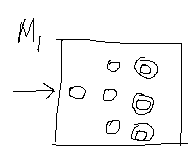
\includegraphics{2-5}
\end{center}

What does if mean for a word $W$ to be in $A_1^*$? %Take any finite number of strings, stick them all together, 
$W$ is in $A_1^*$ if we can break it up into pieces that are in the original language $A_1$.

\begin{center}
\includegraphics{diagrams/diags-2}
\end{center}

Every time we get to the an accept state of $M_1$, i.e. we've read a word in $A_1$ and we {\it might} want to start over. So we put $\ep$-transition leading from the accept state to the start state.

\begin{center}
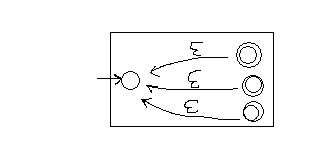
\includegraphics{2-7a}
\end{center}

As in the case with concatenation, we may not want to reset at the first cut point, because maybe there is no way to cut remaining piece into words in $A_1$. So every time get to an accept, have the \emph{choice} to restart---we split into 2 threads, one that looks to continue the current word, and one that restarts.
%Option to restart, can keep doing what.

There is a slight problem: we need to accept the empty string as well. %might be other reasons in start state. 

To do this we add a new start state, and add an $\ep$-transition to the old start state. Then we're good.

\begin{center}
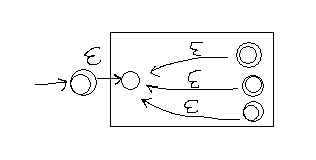
\includegraphics{2-7b}
\end{center} 
\end{proof}

NFA's also give us an easier way to prove closure under union.

\begin{proof}[Proof of closure under $\cup$]
Suppose we're given $M_1$ recognizing $A_1$ and $M_2$ recognizing $A_2$. To build $M$ recognizing $A_1$ and $A_2$, it needs to go through $M_1$ and $M_2$ in parallel. So we put the two machines together, add a new start state, and have it branch by $\ep$-transitions to the start states {\it both} $M_1$ and $M_2$. This way we'll have a finger in $M_1$ and a finger in $M_2$ at the same time.

\begin{center}
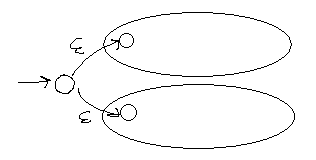
\includegraphics{2-11}
\end{center} 
\end{proof}

\subsection{Converting a finite automaton into a regular expression}
The proof of the closure properties gives us a procedure for converting a regular expression into finite automaton. This procedure comes right out of the construction of machines for $\cup$, $\circ$, and ${}^*$. This will prove part 2 of Theorem~\ref{thm:regex-FA}.
%thm: every regular expression $R$ has an equivalent DFA M.

We do a proof by example: consider $(ab\cup a^*)$. We convert this to a finite automaton as follows. %inductive proof
For $a,b$ we make the following automata. 

\begin{center}
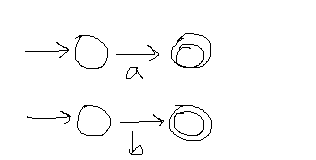
\includegraphics[scale=0.5]{2-8}
\end{center} 

We build up our expression from small pieces and then combine. Let's make an automaton for $ab$. We use our construction for closure under concatenation.

\begin{center}
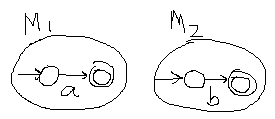
\includegraphics{2-9}\\

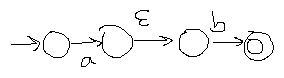
\includegraphics{2-10a}
\end{center} 

This machine recognizes $ab$. Now we do $a^*$.

\begin{center}
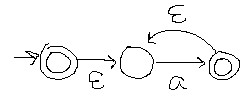
\includegraphics{2-10b}
\end{center} 

%(Closure under union can be proved with nondeterminism, combine with new start state, branching with start state under $\ep$, Fig 11.)
Finally we put the FA's for $ab$ and $a^*$ together, using the $\cup$ construction, to get the FA recognizing $ab\cup a^*$.

\begin{center}
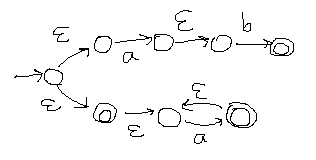
\includegraphics[scale=0.75]{2-10c}
\end{center} 

\cpbox{The constructions for $\cup$, $\circ$, and ${}^{*}$ give a way to construct a FA for any regular expression.}
\lecture{Thu. 9/13/12}

%if M is finite presented
%M: A-mod
%M finite flat
%\implies
%\Leftarrow M finite locally free
%\iff M finite projective
%G \cir X
%finite locally free group scheme /S
%A^m\to A^n\to M\to 0 finite presentations

Today we prove that under the hypothesis on orbits, the geometric quotient is a scheme.

Recall our hypothesis: for all $x\in X$ closed, $G\cdot x\subeq |X|$ is contained in an open affine. We can write $G\cdot x$ another way, as
\[
G\cdot x=\mu(p_2^{-1}(x))
\]

Recall that we defined the geometric quotient $(|X|/\sim,(\pi_*^{\text{top}}\cO_X)^G)\in (RS/S)$, where $\pi^{\text{top}}:|X|\to |X|/\sim$ is the quotient map and  $(\pi_*^{\text{top}}\cO_X)^G$ gives the collection of functions such that $p_2^{\sharp}(a)=\mu^{\sharp}(a)$.

More precisely, thinking of $X$ as a space of functions, the $G$-invariance condition tells us that for $a\in (\pi_*\tp\cO_X)^G$, after pulling back $a$ by the projection and multiplication maps $p_2,\mu:G\times_S X\to X$, we get the same thing: $p_2\sh(a)=\mu\sh(a)$.
\subsection{Geometric quotient, continued}
Our goal today is to prove the following theorem.
\begin{thm} (\cite[4.16]{GGBM}) \llabel{thm:geo-q}
Let $G$ a finite locally free scheme over $S$ and $G\cir X$ be a group scheme action. 
Under the hypothesis on orbits,
\begin{enumerate}
\item
There exists $Y\in \schs$ and $\pi:X\to Y$ such that $(Y,\pi)\cong ((X/G)_{rs},\pi_{rs})$.
\item
$(Y,\pi)$ is a categorical quotient as well.
\item
$\pi:X\to Y$ is integral, quasi-finite, and surjective. (Quasi-finite means that the fibers have dimension 0, i.e. $f^{-1}(y)$ is finite for each point $y\in Y$.)
\item
If $S$ is locally noetherian and $X$ is locally of %locally 
finite type over $S$, then $\pi$ is a finite morphism. %%expect G finite group scheme, or even locally free. Need more condition to get stronger condition (locally free).
%%$Y$ is of finite type over $S$, too.
%if of finite type, then actually Y is of finite type over S.
\item The formation of the quotient (geometric or categorical) commutes with flat base change, namely base change to $S'$ where $S'\to S$  is flat.\footnote{A flat morphism $X\to Y$ is a morphism such that the induced map on every stalk is a flat map of rings, i.e. $f_p:\cO_{Y,f(p)}\to \cO_{X,p}$ is flat for all $p\in X$.} Namely, letting $X':=X\times_S S$, we have 
\[
(G\bs X)_{rs}'\cong (G'\bs X')_{rs}.
\]
\end{enumerate}
\end{thm}
If we have a group action $G$ on $S$, to form a quotient over $S'$ there are two things we can do. 
\begin{enumerate}
\item
Base change to $S'$ and take the quotient, or
\item
take the quotient and base change.
\end{enumerate}
The last point says that we have a natural isomorphism between these two objects.
%The proof tells us a lot about 
\begin{rem} (\cite[4.6]{GGBM}
The condition that $G$ be finite (over $S$) is essential. 
Consider 
\[
\G_m\cir \A_k^1=\G_m\cup \{0\},
\]
where $S=\Spec k$ and $k=\ol{k}$. The categoric quotient is $\A_k^1\to \Spec k$, but the geometric quotient does not exist (the quotient map would have to map $\A_k^1\bs \{0\}$ to a single point; since this is dense it maps all of $\A_k$ to a single point; but there whould be two points because there are two orbits). 
%On 0 it is whole stabilizer. We cannot reconcile this in the categorical quotient. 
There doesn't exist a categorical quotient, but we suspect some quotient might still exist.
\end{rem}

\begin{proof}[Proof sketch]
(See~\cite[4.18--4.25]{GGBM} for the details.)

We first reduce to the affine case by using the hypothesis to show $X$ can be covered by $G$-stable open affine subschemes. We use that $G$ is finite locally free in the reduction step. See~\cite[4.18--19]{GGBM}. %(We also use the fact that $G$ is finite locally free.)

%cover G by G-stable open affine subscheme, reduced to G affine. 
In the affine case $G=\Spec R$, $X=\Spec A$, $S=\Spec Q$. 
$R$ is locally free over $Q$. By localizing, we may assume $R$ is finite free of rank $r$ over $Q$.
Now 
\[
\xymatrix{
G\times_S X \ar@/^/[r]^-{p_2}\ar@/_/[r]_-{\mu} & X
}
\text{ induces }
\xymatrix{
R\ot_Q A &\ar@/^/[l]^-{\mu}\ar@/_/[l]_-{p_2}  A
}
\]
Define 
\[B:=\set{a\in A}{p_2^{\sharp}(a)=\mu^{\sharp}(a)}.\]
\prt{1--3}
We will show that ($Y=\Spec B$, $X\xra{\pi} Y$),  where $\pi$ is induced by $B\hra A$, is the geometric quotient. One main step is the following.

\begin{clm} (\cite[4.20]{GGBM}) \llabel{clm:787-3-1}
$A$ is integral over $B$. 
\end{clm}

We want to produce a monic polynomial with $a\in A$ as root. We have that $\mu^{\sharp}(a)$ acts by multiplication on 
$R\ot_Q A$, a free $A$-module of rank $r$. Let $\chi(X)$ be the characteristic polynomial in $A[X]$.

Observe that $\mu^{\sharp}$ is injective because we have $\mu\circ (e,\id_X)=\id$: 
\[
\xymatrix@R-24pt{S\times_S X=X\ar[r]^-{(e,\id_X)}\ar@/^2pc/[rr]^{\id} & G\times_S X \ar[r]^{\mu}& X\\
x \ar@{|->}[r] & (e,x) \ar@{|->}[r] & x}
\]
On rings, we have $(e,\id_X)^{\sharp} \circ \mu^{\sharp} =\id$, so $\mu^{\sharp}$ is injective.

%Produce monic polynomial which has $a$ as root, in indirect way. 
If suffices to prove $\chi(X)\in B[X]$. By Cayley-Hamilton, $\chi(\mu^{\sharp}(a))=0$. 
Now, we can switch $\chi$ and $\mu\sh$ exactly when the coefficients are in $B$; for $b\in B$, $\mu^{\sharp}(b)=1\ot b=p_2^{\sharp} (b)$. 
%Since $\chi$ has coefficients in $B$ (the ``invariant" ring), this implies 
The fact that $\chi(X)\in B[X]$ gives $\mu\sh(\chi(a))=0$, which, by injectivity of $\mu\sh$, gives $\chi(a)=0$.
%switch ci and musharp exactly when in B, tell you coeff staisfy $\mu^{\sharp}(b)=1\ot b=p_2^{\sharp} (b)$. 
%IMPLIES with $\chi(X)\in B[X]$ above, $\mu^{\sharp}(\chi(a))=0$ implies $\chi(a)=0$.

This shows $a$ is integral over $B$, which is exactly what we want to prove.

Let's prove $\chi(X)\in B[X]$. We need to show 
\beq{eq:chi-in-B[X]}
p_2\sh(\chi(X))=\mu\sh(\chi(X))
\eeq
in $R\ot_Q A[X]$. We write
\[
\chi(X)=(\mu\sh(a)\cir R\ot_Q A\text{ as $A$-module}). 
\]
to mean that $\chi(X)$ is the characteristic polynomial of multiplication-by-$\mu\sh(a)$ on $R\ot A$ considered as a $A$-module. To show~\eqref{eq:chi-in-B[X]}, we transfer $\chi(X)$ to a characteristic polynomial on $R\ot_QR\ot_Q A$ in two ways, and show they are equal.
\begin{enumerate}
\item
We first transfer the action of $A$ on $R\ot_Q A$ to an action of $R\ot_Q A$ on $R\ot_QR\ot_Q A$ via the horizontal maps $p_2\sh$ and $m\ot \id$:
\[
\commsq{A}{R\ot_QA}{R\ot_Q A}{R\ot_Q R\ot_Q A.}{p_2\sh}{p_2\sh}{1\ot \id}{m\ot \id}
\]
From this we get
\beq{eq:787-3-1}
p_2\sh(\chi(X))=((m\ot 1)(\mu\sh(a))\cir R\ot_Q R\ot_Q A \text{ as }R\ot_Q A\text{-module}).
\eeq
\item
Next we transfer the action of $A$ on $R\ot_QA$ to an action of $R\ot_Q A$ on $R\ot_QR\ot_Q A$ via the horizontal maps $\mu\sh$ and $\id \ot \mu\sh$:
\[
\commsq{A}{R\ot_QA}{R\ot_Q A}{R\ot_Q R\ot_Q A.}{p_2\sh}{\mu\sh}{1\ot \id}{\id\ot\mu\sh}
\]
From this we get
\beq{eq:787-3-2}
\mu\sh\chi(X)=((1\ot \mu\sh)(\mu\sh(a))\cir R\ot R\ot A\text{ as }R\ot A\text{-module}).
%p_2\sh(\chi(X))=((1\ot p_2\sh)(\mu\sh(a))\cir R\ot_Q R\ot_Q A \text{ as }R\ot_Q A\text{-module}).
\eeq
Here, $R\ot A$ acts on the 2nd and 3rd coefficients of $R\ot_QR\ot_QA$.
\end{enumerate}
%acting on $R\ot R\ot A$ (a $R\ot A$-module, 2nd and 3rd component).

%We have 
%
%$r\ot a\in R\ot A\mapsto r\ot 1\ot a\in R\ot R\ot A$; $1\ot p_2\sh$ too.  $p_2\sh(a)=1\ot a$. 
%
%The right hand side is $\chi((1\ot \mu\sh)(\mu\sh(a))\cir R\ot R\ot A)$ ($R\ot A$-module). $r\ot a\mapsto r\ot \mu\sh(a)$. We want to show the characteristic proofs are the same. 
The group action axiom
\[
\commsq{G\times G\times X}{G\times X}{G\times X}{X}{1\ot \mu}{m\ot 1}{\mu}{\mu}
\]
now gives
\[
(1\ot\mu\sh)(\mu\sh(a))=(m\sh \ot 1)(\mu\sh(a)).
\]
This means~\eqref{eq:787-3-1} and~\eqref{eq:787-3-2} are equal, and we get~\eqref{eq:chi-in-B[X]}, as needed. This proves Claim~\ref{clm:787-3-1}.\\
%\[
%\xymatrix{
%R\ot A\ar[rr]^{m\sh\ot 1}\ar[rd]_{1\ot p_2\sh} && R\ot R\ot A\\
%& R\ot R\ot A \ar[ru]^{\psi}_{\cong}&
%}
%\]
%The maps are $r\ot a\mapsto r\ot 1\ot a$, $r_1\ot r_2\ot a\mapsto (m\sh(r_1)\ot 1)(1\ot r_2\ot a)=m\sh(r)\ot a$.
%%is it is of 1st 2comp. 
%
%Magic: $\psi$ is an isomorphism
%\bal
%R\ot R&\xrc R\ot R\\
%r_1\ot r_3&\mapsto m\sh(r_1)(1\ot r_2)
%\end{align*}
%This is dual to
%\bal
%G\times G&\xra{(m,p_2)} G\\
%OOPS!&erased
%\end{align*} 
%%work on T-points. abstract groups-> iso.
%We've shown that
%\[
%(1\ot \mu\sh)(\mu\sh(a))=\underbrace{\psi}_{\text{automorphism}}\circ (1\ot p_2\sh(\mu\sh(a)))
%\]
%in $R\ot A$-mod.
%2 elements differ by automorphism, get same characteristic polynomial. Twisting by automorphism is just changing basis. So
%\[
%p_2(\chi(X))=\mu\sh(\chi(X)).
%\]
%Hence $A$ is integral over $B$.

We know $A$ integral over $B$, so $X\to Y$ is integral. By basic facts in commutative algebra, $\pi$ is quasi-finite, closed, and surjective. (See for instance Chapter 5 of Atiyah-MacDonald.) Namely, use Cohen-Seidenberg theory: Going up gives surjectivity, etc.

%From the fact that $A$ is integral over $B$, we can use Cohen-Seidenberg theory (going up, incomparability) and show that
It is not hard to show from here
\[
(Y=\Spec B,\pi:\Spec A\to \Spec B)\cong (|X|/\sim,(\pi_*^{\text{top}}\cO_X)^G)
\]
and that this is the categorical quotient. 
%For instance, going up gives surjectivity of the map $\Spec A\to \Spec B$. 
For details, see~\cite[4.21--22]{GGBM}.\\
%similar to toy model when $S=\Spec k$, $G$ is group or constant group scheme, checked geometric quotient.\\

\prt{4}
Let $G$ be a locally finite type over $S$. Again reduce to the affine case. We can assume that $A$ is a finite $B$-module. $X=\Spec(A)$, $Y=\Spec(B)$, $S=\Spec(Q)$, and $A$ is a finitely generated $Q$-algebra. Then %b q-alg, fin gen b-alg
Because $A$ is finitely generated $Q$-algebra, $A$ is also a finitely generated $B$-algebra. Since $A$ is integral over $B$, this means that $A$ is finitely generated $B$-module, so $\pi$ is finite.\\

%Proof of 2 formal, compare ringed spaces.
%Categorical quotient in ringed spaces, not necessarily schemes. Compart cat quo in ringed spaces vs. scheme. \\

\prt{5}
Reduce to the affine case; suppose $\Spec Q'=S'\to S=\Spec Q$ is flat.
%The intuition is that it comes down to:  Take $G$-invariance over $S=\Spec$ of something, then base change, or...
Say $X=\Spec A$. A function on $X$ is given by $a\in A$. A $G$-invariant element is given by $(p_2^{\sharp}-\mu^{\sharp})(a)=0$. This operation commutes with base change in the following sense:
\[
\ker((p_2^{\sharp}-\mu^{\sharp})\ot_Q Q')=\ker((p_2^{\sharp}-\mu^{\sharp}))\ot_Q Q'
\]
We simply use the fact that tensoring by something flat is an exact functor. %For details, see~\cite[GGBM]{4.}.
\end{proof}
%int'l quasi-finite surjective.

\subsection{Free group actions}
We haven't imposed any conditions on the action itself. The group action is nicer when every point has trivial stabilizer. Our actual definition of a free group action is the following.
\begin{df}
The group action $G\cir X$ where $G\in\gps$ and $X\in \schs$ is \textbf{(strictly) free} if 
\bal
(\mu,p_2):G\times_S X&\to X\times_S X\\
(g,x)&\mapsto (gx,x)
\end{align*}
is a closed immersion.
\end{df}

There is a special case where the action is always free.
\begin{lem}%abelian scheme over S
Let $G\subeq H$ be a closed subscheme in $\gps$. Let $G\cir H$ act by left translation. Then this action is strictly free.
\end{lem}
\begin{proof}
We have
\[
\xymatrix@R-24pt{G\times_S H\ha{r}& H\times_S H\ar[r]^{\cong} & H\times_SH\\
&(h_1,h_2) \ar@{|->}[r] & (h_1h_2,h_2).
}%locally free and flat
\]
where the left map is the basechange of $G\hra H$, hence closed.
\end{proof}

When we impose more conditions on the action, we get stronger results, such as the following theorem (which we won't prove in complete generality)
\begin{thm}\llabel{thm:gsx=xyx}
Let $G\cir X$ be a strictly free group action, $G$ be finite locally free, and $X$ be locally free of finite type. Suppose that the hypothesis on $G\cdot x$ is satisfied. Let $Y$ be the geometric quotient. Then 
\begin{enumerate}
\item
$X\to Y$ is finite and locally free.
\item
We have the following factorization.
\[%finite flat subgroup scheme (ex. torsion)
\xymatrix{
G\times_S X\ar[rd]_{\cong}\ha{rr}^{(\mu,p_2)} && X\times_S X\\
&X\times_Y X\ha{ru}_{\text{closed}}&
}
\]
\end{enumerate}
\end{thm}
\begin{proof}
We can check this locally. Let $X=\Spec A$, $Y=\Spec B$, $S=\Spec Q$, and $G=\Spec R$. Suppse $R$ is free over $Q$ of rank $r$. 

Because $G\times_S X\hra X\times_S X$ is a closed immersion, the corresponding map on rings is surjective: 
\[R\ot_QA\twoheadleftarrow A\ot_Q A .\]  Because $b\in B$, we have $\mu\sh(b)=p_2\sh (b)$ so
\[
\mu\sh(a_1\cdot b)p_2\sh(a_2)=\mu\sh(a_1)p_2\sh(b\cdot a_2).
\]
This means that we can move $b$ between the two factors in $A\ot_Q A$ without affecting the image in $R\ot_Q A$, i.e. we can factor
%
%
%Given $A\ot_Q A\rra R\ot_Q A$ where $a_1\ot a_3\mapsto\mu\sh(a_1)(1\ot a_2)$ and $1\ot a_2=p_2\sh(a_2)=1\ot a_2$ we have factor
\beq{eq:787-3-3}
\xymatrix{
R\ot_Q A &&A\ot_Q A \sj{ll}\ar[ld]_q\\
& A\ot_BA\ar[lu]_{\ph}&
}
\eeq 
%upperright p_2\sh(a_2).
%Can move $b$ between the two factors, so factor through. 
%Because 
The diagram shows $\ph$ is onto. We want to show that $A$ is locally free over $B$. %To do this, we localize at a prime over $B$. 
To do this, we localize at a prime $\mq\sub B$.

$A_{\mq}$ is semilocal (has a finite number of maximal ideals) since $X\to Y$ is quasi-finite.
%finitely many maximal ideals

We show that $A_{\mq}$ is free of rank $r$ over $B_{\mq}$. This fact that $A$ is locally free of rank $r$ over $B$ gives that $A$ is free of rank $r$ over $B$. See~\cite[4.25]{GGBM} for details. 

We get part 2 because we know $\ph$ is onto by~\eqref{eq:787-3-3}. It is enough to show $(\ker\ph)_{\mq}=\ker \ph_{\mq}$ is 0. Using Nakayama's Lemma we can work over $B_{\mq}/\mq$-modules; $B_{\mq}/\mq$ is a field. A vector space map of dimension $r$ that is onto must be an injection. We get $\ker\ph_{\mq}=0$ for all $\mq$, so Nakayama's lemma gives that the kernel itself is 0. 
\end{proof}
%to Mumford, easier, over fields.
\lecture{Tue. 9/18/12}

The course website is
\url{http://math.mit.edu/\~tfei}. The first homework is due on Tuesday of next week.

Recall that to differentiate a vector field in the directino of another, we needed to identify different vector spaces; one way to do so was with the Lie derivative. Another way is to equip the manifold with extra structure, a Riemannian connection. We'll cover this today, and show how from an affine connection we can also define the covariant derivative, which is a generalization of differentiating a vector field along a curve.

\subsection{Affine connection}

For $M$ a smooth $n$-dimensional manifold, let $\X(M)$ be the set of vector fields on $M$.

\begin{df}
An \textbf{affine connection} on $M$ is a function $\nabla:\X(M)\times \X(M)\to \X(M)$ with the following properties.
\begin{enumerate}
\item
$\nabla_Z(X+fY)=\nabla_ZX+Z(f)Y+f\nabla_ZY$
\item
$\nabla_{X+fY}Z=\nabla_XZ+f\nabla_YZ$.
\end{enumerate}
\end{df}
\begin{ex}\llabel{ex:Rn-ac}
The affine connection on $\R^n$ is given as follows. Suppose $X=\sui a_i\pd{}{x_i}$ and $Y=\sui b_i\pd{}{x_i}$. Then
\[
\nabla_XY=\suij a_{i}\pd{b_j}{x_i}\pd{}{x_j};
\]
i.e. the affine connection is just differentiating $(b_1,\ldots, b_n)$ in the direction of $X$.
%$X,Y,Z$ vector fields on $\R^u$ vector valued functions. $Y(X)=dX(Y)$.
\end{ex}
%$X,Y,Z\in X(M)$. $f:M\to \R$ smooth function on $M$.

Note an affine connection basically tells us how to differentiate one vector field with respect to another.

\begin{df}
Suppose $M^n$ is a smooth manifold, $\nabla$ is a connection, and $c:I\to M$ is an interval. A \textbf{vector field} $V$ along the curve $c$ is a function such that for $t\in I$, $V(t)\in T_{c(t)}M$ and $t\mapsto V(t)$ is smooth. 
\end{df}
Note $V(t)$ is not necessarily the restriction of a vector field on $M$, but is a vector field along the curve. For instance, the velocity field along the following self-intersecting curve is a vector field along the curve that is not the restriction of a vector field on $\R^2$. This is becaue at the point of intersection, there are two vectors.
%only bad case.

\begin{center}
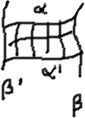
\includegraphics{5-1}
\end{center}

\begin{df}\llabel{df:covar-der}
Let $c:I\to M$ be a smooth curve and $\nabla$ be a connection. There is a unique operation $\fc{D}{\partial t}$ called the \textbf{covariant derivative} along the curve (sending vector fields along the curve to vector fields along the curve) with the following properties.
\begin{enumerate}
\item (Additivity and Leibniz rule)
If $V,W$ are vector fields along the curve and $f:I\to \R$, then
\[
\fc{D}{\partial t}(V+fW)= \fc{D}{\partial t}V+f\fc{D}{\partial t}W+f'W.
\]
\item If $X\in \X(M)$ then
\[
\fc{D}{\partial t}X=\nabla_{c'}X.
\]
\end{enumerate}
\end{df}
%convention
%at the field, if vector field on manifold, capital X,Y,Z. vector field on curve V, W
Think of this as the derivative of a vector field along the curve.

\begin{pr}
Suppose $\nabla$ is a connection, $X,Y,Z\in \X(M)$, and $p\in M$. If $X(p)=Y(p)$, then 
\[
(\nabla_X Z)(p)=(\nabla_Y Z)(p).
\]
\end{pr}
Consider the canonical connection on $\R^n$ as in Example~\ref{ex:Rn-ac}, %The model for a connection: vector field is vector-valued function. The canonical connection on $\R^n$ is 
$\nabla_YX%=Y(X)
=dX(Y)$. %; it has the required properties.
If you evaluate at $p$, it depends on what $X$ is close to $p$, but as for $Y$, it only depends on the value of $Y$ at $p$.

\begin{proof}
Use the fact
\[
\nabla_{X+fY}Z=\nabla_XZ+f\nabla_YZ.
\]
Suppose we have local coordinates $(x_1,\ldots, x_n)$ on $M$. Write $X=a_i\pd{}{x_i}$ and $Y=b_i\pd{}{x_i}$ (repeated indices are summed) where $a_i$ and $b_i$ are smooth functions on $M$. Now by linearity in the subscript,
\[
\nabla_XZ=\nabla_{a_i\pd{}{x_i}}Z=a_i \nabla_{\pd{}{x_i}}Z,
\]
and the same is true for $Y$. Evaluating at $p$, we get that they are equal at $p$.
\end{proof}
\begin{df}
Given local coordinates on a manifold with an affine connection, define the \textbf{christoffel symbols} as the constants $\Ga_{ij}^k$ that make the following true:
\[
\nabla_{\pd{}{x_i}}{\pd{}{x_j}}=:\Ga_{ij}^k \pd{}{x_k}.
\]
\end{df}

If we have two vector fields $X$ and $Y$, writing $X=a_i\pd{}{x_i}$ and $Y=b_j\pd{}{x_j}$, then
\bal
\nabla_X Y&=\nabla_{a_i\pd{}{x_i}}\pa{b_j\pd{}{x_j}}\\
&=a_i\nabla_{\pd{}{x_i}}\pa{b_j\pd{}{x_j}}\\
&=a_ib_j\nabla_{\pd{}{x_i}} \pd{}{x_j}+a_i\pd{}{x_i}(b_j)\pd{}{x_j}\\
&=a_ib_j \Ga_{ij}^k \pd{}{x_k}+a_i\pd{}{x_i}(b_j)\pd{}{x_j}.
\end{align*}
Note in the case of $\R^n$ that $\Ga_{ij}^k=0$ for all $i, j, k$.

\subsection{Covariant derivative}
\begin{proof}[Proof of existence and uniqueness of Definition~\ref{df:covar-der}]
Given an affine connection $\nabla$, $c:I\to M$, and $\nabla$, $V$, $W$ vector fields along $c$, $X\in \X(M)$, $\fc{D}{\partial t}$ is another vector field along $c$.

From the condition $\cvd X=\nabla_{c'} X$, if we want to know value at some point, than we just need to know the velocity at that point. %Extend it to any vector field, value will be the same.

Given $V=a_i\pd{}{x_i}$, $a_i:I\to \R$, we must have 
\beq{eq:965-4-1}
\cvd V=a_i'\pd{}{x_i}+a_i\cvd \pa{\pd{}{x_i}}=a_i'\pd{}{x_i}+a_i\nabla_{c'} \pd{}{x_i}
\eeq
where in the last equality we used that $\pd{}{x_i}$ is a global vector field.
We've shown that $\cvd$ only defined one way, by~\eqref{eq:965-4-1}. Conversely, if $\cvd$ is defined by this, it is easy to see that it has the right properties.
\end{proof}


\begin{df}
Given a manifold $M$, a curve $c:I\to M$, an affine connection $\nabla$, and the corresponding covariant derivative $\cvd$,
we say that a vector field $V$ along $c$ is \textbf{parallel} if
\[
\cvd V=0.
\]
\end{df}
Writing $a:I\to \R$, $V=a_i\pd{}{x_i}$, $c'=c_j'\pd{}{x_j}$, we have
\bal
\cvd V&=a_i'\pd{}{x_i}+a_i\nabla_{c'} \pd{}{x_i}\\
&=a_i'\pd{}{x_i} +a_ic_j'\Ga_{ji}^k \pd{}{x_k}.
\end{align*}
To say that $V$ is parallel is just saying 
\bal
0&=a_i'\pd{}{x_i} +a_ic_j'\Ga_{ji}^k \pd{}{x_k}\\
\iff 0&=(a_{\ell}'+a_ic_j'\Ga_{ji}^{\ell})\pd{}{x_k}\\
\iff 0&=a_{\ell}'+a_ic_j'\Ga_{ji}^{\ell}\text{ for all }\ell.
\end{align*}
This is an ODE! Thus, if we prescribe what the $a_i$ are initially, then by existence and uniqueness of solutions to a first-order linear ODE, we have the following proposition.


%\fixme{Figure 2.}
\begin{pr}\llabel{pr:parallel-vf}
Let $c$ be a curve $I=[0,1]\to M$. 
For each value $V(0)\in T_{c(0)}$, there exists a unique vector field $V$ along $c$ that is parallel and initially has this value.

If $V$ and $W$ are parallel, then $V+\la W$ is also parallel.
\end{pr}

\begin{center}
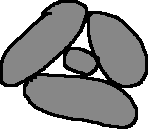
\includegraphics[scale=0.5]{4-2}
\end{center}

\begin{df}
Let $c:I=[0,1]\to M$ be a curve. Define the \textbf{parallel transport} map 
\[
P:T_{c(0)}M\to T_{c(1)}M
\]
as follows. For $v\in T_{c(0)}M$, let $V$ be a parallel vector field along $c$ with $V(0)=v$. Define
\[
P(v)=V(1).
\]
\end{df}
$P$ is a linear map by Proposition~\ref{pr:parallel-vf}.
%Suppose $T_{c(0)}\xra{P}T_{c(1)}M$. $\vartheta\in T_{c(0)} M$, $P(v)=V(1)$. $V(0)=v$, $V$ is parallel. $P$ is a linear map by proposition above. 

%trivial in linear space
\begin{ex}
%How to think about this. 
Take a curve in a plane; think of the plane as a manifold. Take a vector at one end of the curve. What vector on the other end of the curve does it make sense to identify the vector with? The same one!

The vector at the other end does not depend on curve. But, in general, parallel transport depends on the curve. For instance, consider the case of a sphere.

\ig{4-3}{0.5}

In fact, we will see later that the difference is given by the curvature. 
\end{ex}
\cpbox{An affine connection and a curve allows us to identify the  tangent space at one point with the tangent space of another point.\\

It also allows us to differentiate one vector field in the direction of another.}

\vskip0.15in

%Consider a sphere. The identification depends very much on the curve. In fact the difference is given by the curvature. 
In general, without a given curve, we cannot identify tangent spaces at different points without imposing coordinates. If we have a curve, though, we get at least one way to identify those tangent spaces. %, if you have curve. Kind of universal.

Suppose again that we have $M,\nabla,c$, $\cvd(V)$. Suppose for convenience that $c:[0,1]\to M$. Write $V=a_i\pd{}{x_i}$.
Suppose that at $c(0)$, $X_1,\ldots,X_n$ is a basis for $T_{c(0)}$. Then there exists a unique $X_i(t)$ defined as follows:
\[
X_i(t)=P_{c|_{[0,t]}}X_i.
\]
%Note we defined $P:T_{c(0)}M\to T_{c(1)}M$, but we could 
We get $n$ vector fields along the curve. At each point on the curve $c$ that $\{X_i(t)\}_i$ are linearly independent. To see this, note that they are linearly dependent initially, and that by uniqueness in Proposition~\ref{pr:parallel-vf}, parallel translation is symmetric; going forwards and then backwards on the curve gives the identity. If the $X_i(t)$ were linearly dependent at time $t$, we can parallel transport backwards to get a linear dependence relation at time $t=0$, contradiction. %get non-uniqueness of solution.

We can write any vector field as $V=a_iX_i$ where $a_i$ are smooth functions $I\to \R$. Now %formal nonsense
\[
\cvd V=a_i \cvd X_i+a_i'X_i=a_i'X_i
\]
where the first term is 0 because $X_i$ is a parallel basis. Thus we see that the covariant derivative is especially simple.

Recall that given $M$, $p\in M$, a {\it Riemannian metric} is a smoothly varying inner product on the tangent space.

Other structures are interesting, too: Instead of inner product, we could have indefinite (nondegenerate symmetric bilinear) forms. For example, we could consider a Lorentzian. If you study general relativity, then it's all about the Lorentzian metric. Think about a manifold as both space and time; on space we have a Riemannian metric, and on time, we have another bilinear form that is negative definite.

\subsection{Compatibility of metric and connection}
Note that in our study of connections so far, the metric didn't play a role at all. We now bring in the metric. We want the connection to be compatible with the Riemannian metric.
\begin{df}
Let $(M^n,g)$ be a smooth Riemannian manifold and a connection $\nabla$. We say that $g$ is \textbf{compatible} with $\nabla$ if whenever $c:I\to M$ is a curve and $V$ and $W$ are parallel vector fields along $c$, then $g(V,W)$ is constant along $c$. 
%intuitive
\end{df}
If $C:[0,1]\to M$ and $V(0)\perp W(0)$, then $V\perp W$ everywhere along the curve and $|V||W|$ is constant.

\begin{ex}
Take the canonical example $\R^n$, $\nabla$. Let $g=\an{\cdot,\cdot}$ be the usual inner product. Then the connection is compatible with the metric:
The inner product of parallel vector fields is constant along the curve. 
\end{ex}

%riemannian metric, unique connection. Will prove. Prove defn is equiv to more standard about what compat connection is.
%go through most of book, not ch. 10, for certain, ch. 13, then some topics.
Next time we will prove that any Riemannian metric gives rise to a unique connection, and show that our definition of a connection is equivalent to a more standard definition.
\lecture{Thu. 9/20/12}

Today we will (finally) talk about abelian schemes. We'll start by recalling some terminology from scheme theory.

\subsection{Review of scheme theory}
\begin{df}
\begin{enumerate}
\item
$X\in \pat{Sch}$ is \textbf{locally noetherian} if for all open affine $U\subeq X$, $U=\Spec A$ for some noetherian ring $A$.
\item
$f:X\to Y$ is \textbf{locally of finite type}, \textbf{locally of finite presentation} if for all open affine $V=\Spec A\subeq X$, for all $U=\Spec B\subeq f^{-1}(V)$, $B$ is an algebra of finite type (finitely generated), of finite presentation, respectively.
The first means $V\cong A[x_1,\ldots, x_n]/\ma$, and the second means that in addition $\ma$ is finitely generated.
\item
$f:X\to Y$ is \textbf{quasi-compact} if for all $V\subeq Y$ open affine (quasi-compact), $f^{-1}(V)$ is quasi-compact.
%board falls away. 
\end{enumerate}
\end{df}
%affine quasicompact
%2 equivalent
\begin{rem}It is enough that there exist some open covering that has the property (i.e., the properties are affine-local properties).
\end{rem}
%We want to define these for morphisms.
\begin{df}
A morphism is
\begin{enumerate}
\item
\textbf{noetherian} if it is locally noetherian and quasi-compact.
\item
\textbf{of finite type} if it is locally of finite type and quasi-compact
\item
\textbf{of finite presentation} if it is locally of finite presentation and quasi-compact.
\end{enumerate}
%useful when work outside noetherian schemes.
%work as if on locally noetherian or noetherian scheme.
\end{df}
\begin{pr}
Let $f:X\to Y$ be a morphism such that $Y$ is (locally) noetherian and $f$ is (locally) of finite type. Then $X$ is (locally) noetherian and $f$ is (locally) of finite presentation.
\end{pr}%locally everywhere or without locally everywhere
\begin{proof}
In the affine case, this says that a finitely generated algebra over a noetherian ring is noetherian and finitely presented. This is true by the Hilbert Basis Theorem.

Glue for the general case.
\end{proof}
One of many definitions for smooth is the following.
\begin{df}
$f$ is \textbf{smooth} if $f$ is locally of finite presentation, flat, and has geometrically regular fibers. 

A flat morphism $f:X\to Y$ is one such that if $f(x)=y$, then $\sO_{Y,y}\to \sO_{X,x}$ is a flat algebra.

Geometrically regular fibers means that for all scheme-theoretic points $y\in Y$, %$X_y\xra{f_y}y=\Spec k(y)$ 
the bottom map is regular.

\[
\xymatrix{X_y \ar[r]^-{f_y} & y=\Spec k(y)\\
X_{\ol{y}} \ar[r]^-{\text{regular}} \ar[u] & \Spec \ol{k(y)}\ar[u]}
\]

Regular means that the local rings at every point is regular, i.e. we have the correct dimension for the tangent space at every point.  %(look at the Jacobian).
\end{df}
%fiberwise smooth
\begin{df}
Let $k$ be a field. $X\in \pat{Sch$/k$}$ is a \textbf{variety} if $X$ is integral (reduced and irreducible), of finite type, and separated.
\end{df}

We have the following fact.
\begin{fct}
$X\times_k k'$ is reduced/irreducible/connected for all field extensions $k'/k$ iff $X\times_k\ol{k}$ is reduced/irreducible/connected for some algebraic closure $\ol{k}$. We say that $X$ is \textbf{geometrically} reduced/irreducible/connected.
%true for transcendental too.
\end{fct}
\begin{df}
A morphism $f$ is \textbf{proper} if it is separable, of finite type, and universally closed.
\end{df}
\begin{fct}
Let $k$ be a field, and $X/k$ be proper and geometrically connected and reduced. Then the global sections are
\[H^0(X,\cO_X)\cong k.\]
\end{fct}
\subsection{Abelian schemes}
\begin{df}\llabel{df:787-5-1}
Let $S$ be any scheme. An scheme $A\in \schs$ with $\pi:A\to S\in \schs$ is an \textbf{abelian scheme} if it satisfies either of the following equivalent conditions.
\begin{enumerate}
\item
$\pi$ is smooth, proper, and has geometrically connected fibers (for all $s\in S$, $A_s$ is $G$-connected). %where does geo connected come in?
\item
if $\pi$ is proper, flat, and of finite presentation with smooth geometrically regular fibers.\footnote{A scheme is regular if it is covered by affine opens $\Spec A$ with $A$ regular, i.e., noetherian and such that the localization at every prime ideal is a regular local ring.}
\end{enumerate}
\end{df}
\begin{proof}[Proof of equivalence]
Observe that $(2)\implies (1)$ is by definition: smooth means locally of finite presentation, flat, and having geometric regular fibers.

For $(1)\implies (2)$, everything is clear except finite presentation. Note that a smooth morphism is locally of finite presentation, and a proper morphism is of finite type, hence quasi-compact. A morphism that is locally of finite presentation and quasi-compact is of finite presentation.
\end{proof}
\begin{rem}
``Geometrically" can be removed in condition 1: If $X/k$  is a connected scheme with $X(k)\ne \phi$, then $X$ is automatically geometrically connected. Apply this fact to $X=A_s=\xymatrix{A\times_S \Spec k(s)\ar[r]^{}& \Spec k(s)\ar@/^/[l]^-{e_{A_s}}}$ where $e_{A_s}$ is the identity section.
\end{rem}%fibers usually geom connected.
\begin{df}\llabel{df:787-5-2} (Mumford's definition) Let $k=\ol{k}$. Then an \textbf{abelian variety} over $k$ is a proper group variety over $k$. %int sep of finite type proper over k
\end{df}
We would like an abelian scheme over $\Spec k$ (where $k=\ol k$) that is a variety to be an abelian variety over $k$.
\begin{proof}[Proof of equivalence]
Definition~\ref{df:787-5-1}(1)$\implies$Definition~\ref{df:787-5-2}: Because $X$ is proper, $X$ is separated of finite type. We want $X$ to be integral (reduced and irreducible). We use the following facts for schemes over a field $k$: 
\begin{itemize}
\item
connected and smooth together imply geometrically irreducible,
\item 
smooth implies geometrically reduced.
\end{itemize}•
 Thus an abelian scheme over $k$ is a variety.\\

\noindent
Definition~\ref{df:787-5-2}$\implies$~\ref{df:787-5-1}(1): We use the following fact: Let $X/k$ be reduced and locally of finite type, where $k$ is a perfect field. Then the smooth locus $X_{sm}\subeq X$ is open dense.
%nonsing pts open dense

Now $X_{sm}$ is open dense but also stable under group translation, so $X_{sm}=X$ and $X$ is smooth.
\end{proof}
Thus our definitions~\ref{df:787-5-1} and~\ref{df:787-5-2} are healthy!

An example of an abelian variety is an elliptic curve.
%We now give some examples to appreciate these conditions. It's actually not easy to write down an example.
% For elliptic curve, we can write down $\C/\Z+i\Z$. It's either to give a non-example.

Why do we impose these conditions? To see this, let's look at some nonexamples.
\begin{ex}
%proper group variety is abelian variety.
%every fiber is an abelian variety.
%Non-smooth, non-flat.
%What does smooth do? 
%The key condition if flatness; if we don't impose this then we get stupid examples: Consider $A$ over $\Spec{\fpb}$. Throw it into $\ol{\Z_p}$. 
%\[
%\xymatrix{
%A\ar[d]_{AV/\fpb} \ar[rd] &
%\\
%\Spec\fpb \ha{r} & \Spec \ol{\Z_p}.
%}
%\]
%This is wrong (see SW's remarks, 9/20)
The schemes $\G_{m,S}$, $\G_{a,S}$, and $GL_{n,S}/S$ are not abelian because they are not proper.  ($\G_{m,S}$ and $GL_{n,S}/S$ are not of finite type, while $\G_{a,S}$ is not universally closed.)

The constant group scheme $(\Z/n\Z)_S$ is not an abelian scheme: it is smooth and proper but not geometrically connected. It has $n$ points over each %geo
fiber.
\end{ex}

\subsection{Rigidity lemma and applications} %shows that abelian schemes are abelian}

So far we haven't imposed a condition that the group law be abelian. A natural question is: if the group law abelian for abelian schemes? Yes; our definitions in fact force it to be abelian, but the proof is somewhat technical, relying on the following lemma.
\begin{lem}[Rigidity lemma]\llabel{lem:rigid}
Let $X,Y,S$ be locally noetherian (over $S$), let $f:X\to Y$ be a morphism, and let $e:S\to X$ be a section. Suppose $p:X\to S$ is proper and flat (with geometrically reduced fibers?), $S$ is connected, $q$ is finite separated, and $p\circ e=\id_S$. We have the following diagram
\[
\xymatrix{
X\ar[rr]^f\ar@/_1pc/[rd]_p & & Y\ar[ld]^q\\
& S\ar[lu]_e. & 
}
\]
If $f(X_s)=\{y\}$ as a set for some $s\in S$, then $f=\eta \circ p$ where $\eta=f\circ e$, and $S\to Y$ is a section of $q$.
\end{lem}
In other words, when we impose a property for one fiber, then we get the property over all S. We'll postpone the proof to next lecture, and focus instead on the consequences.\\

\cpbox{The rigidity lemma allows us to take a property over one fiber of $S$ and show it holds over all of $S$.}

\begin{cor}\llabel{cor:rigid1}
Suppose we have scheme morphisms
\[
\xymatrix{
A\ar@/^1pc/[rr]^f\ar[rr]_g\ar@/_1pc/[rd]_p & & G\ar[ld]^q\\
& S\ar[lu]_{e_A}. & }
\]
where $A$ is an abelian scheme, $q:G\to S$ is separated of finite presentation, and $f,g$ are morphisms in $\schs$ (not necessarily in $\gps$). If for some $s\in S$, $f_s=g_s$, then $f=\mu_{G}\circ ((\eta\circ p)\times g)$ for some section $\eta:S\to G$ (in fact $\eta=f\circ e_A$).
%note too difficult deduce.
\end{cor}
The idea is as follows. We can take a difference of morphisms, because $G$ is a group scheme. We have that ``$f-g$" is constant over a fiber; hence by the rigidity lemma it is constant everywhere.
\begin{proof}
%don't assume locally noeth, but can always reduce to noeth cse. 
By generalities in EGA IV we can reduce to the locally noetherian case. We can apply the rigidity lemma to 
\[
A\xra{(f,i_G\circ g)}  G\times_S G \xra{\mu} G
\]
sending
\[
x\mapsto (f(x),g(x)^{-1})\mapsto f(x)g(x)^{-1}.
\]
We have $h(A_s)=\{e_G(s)\}$ (the identity on $G$). By the rigidity lemma, $h=\eta\circ p$ and $\eta=h\circ e_A$. 
Another way to write this is $f=\mu_G\circ ((\eta\circ p)\times g)$.\footnote{Taking $T$-points, we have $f(x)g^{-1}(x)=h(e_A)$ becomes $f(x)=g(x)h(e_A)$. This is equivalent to saying $h=\mu_G\circ (f,i_G\circ g)=\mu_G\circ (f,i_G\circ g)\circ e_A\circ p$ implies $f=\mu_G\circ (\mu_G\circ (f,i_G\circ g)\circ e_A\circ p,g)=\mu\circ (f\circ e_A\circ p,g)$.} 
%\fixme{Then we can check $f=\mu\circ ((\eta\circ p)\times g)$ (on $T$-points). This means $f-g$ is constant.}
\end{proof}
\begin{cor}\llabel{cor:rigid2}
Suppose $A$ is an abelian scheme over $S$ and $G$ is finite separated group scheme over $S$:
\[
\xymatrix{
A\ar[rr]^h \ar[rd]_{\text{abelian scheme}}& & G\ar[ld]^{\text{finite separated}}\\
& S. &
}
\]
If $h$ sends the identity element of $A$ to the identity element of $G$, i.e. $h\circ e_A=e_G$, then $h$ is a group homomorphism.
\end{cor}

%don't need connectedness, argue on each component.
\begin{proof}
Let $p,q$ be the projections to the first component. Apply Corollary~\ref{cor:rigid2} to
\[
\xymatrix{
A\times_S A \ar@/^1pc/[rr]^f\ar@/_1pc/[rr]_g \ar[rd]_p& & A\times_S G\ar[ld]^q\\
%S\ar[r]^{e_A}
& A &
}
\]
%pull back by id section, like taking $x_1$ to be identity.
where we let $f$ and $g$ be the maps
\begin{align*}
(x_1,x_2)&\mapsto(x_1,h(x_1x_2))\\
(x_1,x_2)&\mapsto(x_1,h(x_2))
\end{align*}
and $p,q$ are projections onto the first component. 
Note that $p=q\circ f$. %$x_1$ downstairs, in $A$.

%Identity, see on level of points

%\fixme{Pullback via $S\xra{e_A}Z$. We have $f\times e_A=g\times e_A$ where $x_1=\id$ (?). Apply corollary 1 to get
The corollary gives
\[
f=\mu_G\circ ((\eta \circ p)\times g)
\]
%and unravel to get (Note $G$ is a group scheme with group law. $A\times_S\mu_G$.)
%p,q  to 1st compo.
Unraveling the definitions, we get  
\bal
(x_1,h(x_1x_2))&=(x_1,\eta_0(x_1))\cdot_{G} (x_1,h(x_2))\\
\implies h(x_1x_2)&=\eta_0(x_1)h(x_2).
\end{align*}
Take $x_2=\id$ to get $h(x_1)=\eta_0(x_1)$. Hence we get \[h(x_1x_2)=h(x_1)h(x_2).\]
\end{proof}
%I.e. a morphism sending the identity to the identity must be a group homomorphism.

Now we show that an abelian scheme is well-named.
\begin{cor}
Let $A\to S$ be an abelian scheme. Then $A$ has commutative group law.
\end{cor}
\begin{proof}
Commutativity is equivalent to the the inverse map $x\mapsto x^{-1}$ being a homomorphism. 
Apply Corollary~\ref{cor:rigid2} to $A\xra{i_A} A$, $x\mapsto x^{-1}$. This morphism sends $e_A$ to $e_A$ so it is a group hoomorphism. Hence $A$ is abelian.
\end{proof}
For example, consider an elliptic curve, which is a smooth proper genus 1 curve. Choose a basepoint, i.e., declare a point to serve as the identity. Then the group law is determined. We generalize this.
\begin{cor}
Let $(A,e_A,i_A,\mu_A)$ and $(A,e_A,i_A',\mu_A')$ in $\gps$ be two abelian scheme structures on the same scheme, with the same identity element.

Then $i_A=i_A'$ and $\mu_A=\mu_A'$, i.e. the abelian schemes are the same.
\end{cor}
\begin{proof}
Apply Corollary~\ref{cor:rigid2} to $A\xra{\id} A$. It is an automorphism of schemes; hence it is a group homomorphism by the Corollary, and the group structures are compatible.
\end{proof}
We give the proof of the rigidity lemma next time.

\lecture{Thu. 2/17/11}

\subsection{Second Moment Method}
\begin{df}
The \textbf{variance} of a random variable $X$ is
\[
\Var(X)=\E[(X-\E(X))^2]=\E(X^2)-E(X)^2
\]
The standard deviation is
\[
\sigma=\sqrt{\Var(X)}.
\]
\end{df}
\begin{thm}[Chebyshev's Inequality]
For any $\la>0$,
\[
P(|X-\mu|\geq \la \sigma)\leq \rc{\la^2}.
\]
\end{thm}
\begin{proof}
\[\sigma^2=\Var(X)=\E[(X-)^2]\geq \la^2 \sigma^2 P(|X-\mu|^2\geq \la^2\sigma^2).\]
This is Markov's inequality with $Z=(X-\mu)^2$, $\E(Z)=\sigma^2$, and $\la^2$. Now $Z\geq \la^2 \sigma^2$ iff $|X-\mu|\geq \la \sigma$.
\end{proof}
Suppose $X=X_1+\cdots +X_n$. Then
\[
\Var(X)=\sum_{i=1}^n \Var(X_i)+\sum_{i\neq j} \Cov(X_i,X_j)
\]
where
\[
\Cov(X_i,X_j)=E(X_iX_j)-E(X_i)E(X_j).
\]
In particular, if $X_i,X_j$ are independent then
\[
\Cov(X_i,X_j)=0.
\]
Suppose $X_i$ is an indicator random variable, i.e. $X_i=1$ if a certain even $A_i$ occurs and 0 otherwise. If $X_i=1$ with probability $P(A_i)=p$ then $\Var(X_i)=p(1-p)\leq p=\E(X_i)$. Hence
\[
\Var(X)\leq \E(X)+\sum_{i\neq j} \Cov(X_i,X_j).
\]

\subsection{Number Theory}
Let $\nu(n)$ be the number of prime factors of $n$. We will show that almost all $n$ have close to $\ln \ln n$ prime factors.
\begin{thm}[Hardy-Ramanujan]
Let $\omega(n)\to \infty$ arbitrarily slowly. Then the number of $x$ in $\{1,\ldots, n\}$ with $|U(x)-\ln\ln x|>\omega (n)\sqrt{\ln\ln n}$ is $o(n)$. In other words, for $x$ randomly chosen from $[1,n]$,
\[
P(|\nu(x)-\ln \ln n|>\omega(n)\sqrt{\ln\ln n})=o(1).
\]
\end{thm}
\begin{proof}
Let $x$ be randomly chosen from $1$ to $n$. For $p$ prime, let $X_p$ be the indicator random variable for the event $p|x$. Set $M=n^{\rc{10}}$ and $X=\sum_{p\leq M,p\text{ prime}} X_p$. Note
\[
x\leq \nu(x)< x+10.
\]
since a number has less than 10 prime factors greater than $n^{\rc{10}}$. (We exclude the large primes because they will give a greater variance for $X_p$.)
Now
\[
\E(X_p)=\rc{n}\fl{\frac np}=\rc{p}+O\prc{n}
\]
so
\[
\E(X)=\sum_{p} \E(X_p)=\sum_p \pa{\rc{p}+O\prc{n}}
=\ln\ln M+ O(1)=\ln\ln n+O(1)
\]
using Mertens's estimate.

The rough idea is to show that for $p\neq q$, $X_p$ and $X_q$ are almost independent, so the covariances are small, and don't affect the variance of $X$ much. I.e. $\E(X_p\wedge X_q)\approx \E(X_p)\E(X_q)$.
We have
\[
\Var(X_p)=\rc{p}\pa{1-\rc p}+O\prc{n}
\]
so
\begin{equation}\label{numpsumv}
\sum_p\Var(X_p)=\sum_p \rc{p}+O(1)=\ln \ln n +O(1).
\end{equation}
Now $X_pX_q=1$ iff $pq|X$, so
\[
|\Cov(X_p,X_q)|=\ab{\frac{\fl{\frac{n}{pq}}}{n}-\frac{\fl{\frac np}}{n}\cdot \frac{\fl{\frac nq}}{n}}\leq%\rc{pq}-\pa{\rc{p}-\rc{n}}\rc{q}-\rc{n}
\rc{n}\pa{\rc p+\rc q}.
\]
Hence
\begin{equation}\label{numpsumc}
\ab{\sum_{p\neq q}\Cov(X_p,X_q)\leq \rc{n}\sum_{p\neq q}\pa{\rc p+\rc q}}
\leq \ab{\frac{2M}{n}\sum_{\footnotesize \begin{array}{c}p\leq M\\p\text{ prime}\end{array}} \rc{p}}=o(1).
\end{equation}
since we counted each $\rc{p}$ at most $2M$ times.
Putting~(\ref{numpsumv}) and~(\ref{numpsumc}) together,
\begin{align*}
\Var(X)&=\sum_p \Var(X_p)+\sum_{p\neq q} \Cov(X_p,X_q)\\
&=\ln\ln n+O(1).
\end{align*}
Since $\sigma=\sqrt{\ln \ln n}+O(1)$, by Chebyshev's inequality
\[
P(|X-\ln\ln n|\geq \la \sqrt{\ln\ln n})<\la^{-2}+o(1).
\]
and the same holds for $\nu(X)$. Letting $\la\to \infty$ gives the theorem.
\end{proof}
In fact, %an extension of this method shows that 
the 
distribution of $\nu(x)$ approaches a normal distribution with mean and variance $\ln \ln n$.
%$\nu(x)$ behaves like a normal distribution with mean and variancae $\ln\ln n$.
\begin{thm}[Erd\"os-Kac]
Fix $\la\in \R$. Then
\[
\lim_{n\to \infty} |\{x:x\in [n],\nu(x)\geq \ln \ln n +\la\sqrt{\ln \ln n}\}|
=
\int_{\la}^{\infty} \rc{\sqrt{2\pi}}e^{-t^2/2}\,dt.
\]
\end{thm}
For $\la$ large, this is asymptotic to $\sqrt{\frac{2}{\pi}}e^{-\la^2/2}/\la\ll\la^{-2}$.
\begin{proof}(Outline)
Fix $s(n)$, $s(n)\to \infty$, and $s(n)=o(\sqrt{\ln\ln })$ such as $s(n)=\ln\ln\ln n$.\footnote{Drowning number theorists say log log log.}
Set $M=n^{\rc{n}}$ and \[X=\sum_{\scriptsize \begin{array}{c}
p\leq M\\p\text{ prime}
\end{array}}
\]
Then
\[
\nu(x)-s(x)\leq X\leq \nu(x).\]
Let $Y_p$ be independent random variables with $P(Y_p=1)=\rc{p}$ and $P(Y_p=0)=1-\rc{p}$. $Y_p$ represents an idealized version of $X_p$. %that we can apply th Central Limit Theorem to. 
Set
\begin{align*}
\mu&=\E(Y)=\ln \ln n+o((\ln \ln n)^{\rc 2})\\ 
\sigma^2&=\Var(Y)\sim \ln \ln n.\\
\tilde{Y}&=\frac{Y-\mu}{\sigma}.
\end{align*}
By the Central Limit Theorem, $\tilde Y$ approaches the standard normal distribution $N$ and $\E(\tilde{Y}^k)\to \E(N^k)$. %If for all k then approaches normal. prob thm
Let $\tilde X=\frac{X-\mu}{\sigma}$ and compare $\tilde X$ and $\tilde Y$. For distinct primes $p_1,\ldots, p_s$, %the expected value 
\begin{equation}\label{l6-ed}
\E(X_{p_1}\cdots X_{p_s})-\E(X_{p_1})\cdots \E(X_{p_s})=O\prc{n}.
\end{equation}
Fix $k\in \N$. Compare $\E(\tilde{X}^k)$ with $\E(\tilde Y^k)$. Expanding, $\tilde X^k$ is a polynomial in $X$ with coefficient $n^{o(1)}$. Expanding $X^j$, always reducing $X_p^a$ for $a\geq 2$, each $X^j=\pa{\sum X_p}^j$ gives $O(M^k)$ terms equal to $n^{o(1)}$ of the form $X_{p_1}\cdots X_{p_s}$. The same expansion applies to $\tilde Y^k$. As the corresponding terms have expectation within $O\prc{n}$ by~(\ref{l6-ed}),
\[
\E(\tilde X^k)-\E(\tilde Y^k)=o(1).
\]
Thus each moment of $\hat X$ approaches that of the standard normal $N$, giving that (by a theorem from probability) $\hat X$ approaches the normal distribution.
%Prob dist unique determined by moments when exp func integrable -> fourier transform of measure by expanding exponential series e^it. Caman
%Hausdorff normal
\end{proof}
\lecture{Thu. 2/24/11}

\subsection{Distinct sums}
%Distinct sums
\begin{df}
A set $x_1,\ldots, x_k\in \N$ has \textbf{distinct sums} if all sums
\[
\sum_{i\in S}x_i,\quad S\subeq [k]
\]
are distinct.
\end{df}
Let $f(n)$ be the maximum $k$ such that there exists $\{x_1,\ldots, x_k\}\subeq [n]$ with distinct sums. Since $\{2^i|i\leq \log_2 n\}$ has distinct sums,
\[
f(n)\geq 1+\fl{\log_2 n}.
\]
(There are actually sequences that do better, $f(n)\geq 3+\fl{\log_2 n}$ for large $n$.)
%Erdos inflation
%Hang on wall vs. cash it in. How pay out?
Erd\H{o}s asked the following: 
Determine if there is a constant $C$ such that $f(n)\leq C+\log_2 n$. 

If $k=f(n)$, all $2^k$ sums are distinct and at most $kn$, giving $2^{f(n)}\leq f(n)n$, and $f(n)\leq \log_2 n+\log_2\log_2 n+O(1)$.
\begin{thm}
\[
f(n)\leq \log_2 n+\rc{2}\log_2\log_2 n+O(1).
\]
\end{thm}
\begin{proof}
Fix $\{x_1,\ldots, x_k\}\subeq [n]$ with distinct sums. Let $\ep_1,\ldots, \ep_k$ be independent random variables with
\[
P(\ep_i=0)=P(\ep_i=1)=\rc{2}
\]
and set $X=\ep_1x_1+\cdots +\ep_kx_k$. Then $X$ is a random sum, and
\begin{align*}
\mu&=\E(X)=\frac{x_1+\cdots +x_k}{2}\\
\sigma^2&=\Var(X)=\frac{x_1^2+\cdots +x_k^2}{4}\leq \frac{n^2 k}{4}
\end{align*}
since the $X_i=\ep_ix_i$ are independent random variables. ($\Var(X_i)=\E(X_i^2)-\E(X_i)^2=\frac{X_i^2}{2}-\frac{X_i^2}{4}$.) By Chebyshev, (we want to show that a constant fraction of the sums lie in a small region around the mean, and use Pigeonhole to conclude that if there's too many, then two of them are equal)
\begin{align*}
P(|X-\mu|\geq\la\sigma)&\leq \rc{\la^2}\\
P\pa{|X-\mu|\geq\la\frac{n\sqrt k}{2}}&\leq \rc{\la^2} 
\end{align*}
Then
\[
1-\rc{\la^2}\leq P\pa{|X-\mu|<\frac{\la n\sqrt k}{2}}\leq 2^{-k} (\la n\sqrt k +1)
\]
since at most $\la n\sqrt k +1$ of the sums can be in the interval $\pa{
\mu-\frac{\la n\sqrt k}{2},\mu+\frac{\la n\sqrt k}{2}
}$ and each is chosen with probability $2^{-k}$. Take $\la=\sqrt 3$. Then the equation gives $2^k\leq Ck^{\rc 2}n$ for some constant $C$; take logs to get the answer.
\end{proof}

\subsection{Some bounds}
Let $X$ be a nonnegative integer-valued random variable (e.g. $X$ counts something). We want to bound $P(X=0)$ given $\mu=\E(X)$. If $\mu\leq 1$, then
%\sum_{i>0} iP(X=i)\geq \sum_{i>0} P(X=i)=P(X>0).
\[P(X>0)\leq \E(X)\implies P(X=0)\geq 1-\E(X).\]
If $\E(X)\to \infty$, then not necessarily $P(X=0)\to 0$. But if the standard deviation is small relative to $\mu$ this is true. 

\begin{ex}
For example, $X$ be the deaths due to nuclear war in the next year. 
%Stroock, "We should do experiments"
Then $P(X>0)$ is small but $\E(X)$ is large.
\end{ex}

\begin{thm}
Let $X$ be a nonnegative integer-valued random variable. Then
\[P(X=0)\leq \frac{\Var(X)}{\E(X)^2}.\]
\end{thm}
\begin{proof}
Let $\mu=\frac{\mu}{\sigma}$. Then Chebyshev's inequality gives
\[
P(X=0)\leq P(|X-\mu|\geq \la\sigma)\leq \rc{\la^2}=\frac{\Var(X)}{\E(X)^2}.
\]
\end{proof}
\begin{cor}
If $\Var(X)=o(\E(X)^2)$ then %$X>0$ almost always. (i.e. 
$P(X>0)\to 1$. In fact
\[
X\sim \E(X)
\]
almost surely. (For each $\ep>0$, $|X-\E(X)|<\ep\E(X)$ goes to 0 as $X\to \infty$.)
\end{cor}
\begin{proof}
Take $\la=\frac{\ep\mu}{\sigma}$ and let $\ep\to 0$.
\end{proof}
\lecture{Tue. 10/2/12}

%\fixme{Add an introduction (Motivation, etc.)}

\subsection{Curvature}
Let $M^n$ be a Riemannian manifold with Levi-Civita connection $\nabla$. Define the curvature as follows.
%difference, 3rd order der.
\begin{df}
For $X,Y,Z\in \X(M)$ define the \textbf{curvature} operator as follows.
\[
R(X,Y)Z:=\nabla_Y\nabla_X Z-\nabla_X\nabla_Y Z+\nabla_{[X,Y]}Z
\]
\end{df}
Think of this as a difference in second order derivatives. Note there are different conventions for the curvature operator. 

\begin{pr}\llabel{pr:965-8-1}
$R$ is linear in each variable:
\begin{align*}
R(X_1+X_2,Y)Z&=R(X_1,Y)Z+R(X_2,Y)Z\\
R(X,Y_1+Y_2)Z&=R(X,Y_1)Z+R(X,Y_2)Z\\
R(X,Y)(Z_1+Z_2)&=R(X,Y)Z_1+R(X,Y)Z_2
\end{align*}
and for $f\in C^{\iy}(M)$,
\[
R(fX,Y)Z=R(X,fY)Z=R(X,Y)fZ=fR(X,Y).
\]
\end{pr}
Assuming that this is the case, $(R(X,Y)Z)(p)$ only depends on the value of $X$, $Y$, and $Z$ at $p$. Indeed, write $X=a_i\pdd{x_i}$, $Y=b_j\pdd{x_j}$, and $Z=c_k\pdd{x_k}$. Then using linearity in each variable,
\begin{align*}
R(X,Y)Z&=R\pa{a_i\pdd{x_i},b_j\pdd{x_j}}\pa{c_k\pdd{x_k}}\\
&=a_ib_jc_kR\pa{\pdd{x_i},\pdd{x_j}}\pdd{x_k}.
\end{align*}
\begin{proof}
The connection is linear in each variable, so the first set of equations holds.

Now using
\bal
[X,Y]h&=XYh-YXh\\
[fX,Y]h&=fXY(h)-Y(f)X(h)-fYX(h)=f[X,Y](h)-Y(f)X(h)
\end{align*}
we calculate
\begin{align*}
R(fX,Y)Z&=\nabla_Y\nabla_{fX} Z-\nabla_{fX}\nabla_Y Z+\nabla_{[fX,Y]}Z\\
&=\nabla_Y f\nabla_X Z-f\nabla_X\nabla_Y Z+f\nabla_{[X,Y]}Z-Y(f)\nabla_XZ\\
&=\cancel{Y(f)\nabla_XZ}+f\nabla_Y\nabla_X Z-f\nabla_X\nabla_Y Z+f\nabla_{[X,Y]}Z-\cancel{Y(f)\nabla_XZ}\\
&=fR(X,Y)Z.
\end{align*}
The proof for $Y$ is similar; we carry out the proof for $Z$.
\begin{align*}
R(X,Y)(fZ)&=\nabla_Y\nabla_X (fZ)-\nabla_X\nabla_Y (fZ)+\nabla_{[X,Y]}Z\\
&=\nabla_YX(f)Z+\nabla_Yf\nabla_XZ -\nabla_XY(f)Z-\nabla_Xf\nabla_Y Z+[X,Y](f)Z+f\nabla_{[X,Y]}Z\\
&=\cancel{\color{blue}YX(f)Z}+\cancel{\color{red}X(f)\nb_YZ} +\cancel{\color{purple}Y(f)\nb_XZ}+\cancel{f\nb_Y\nb_XZ}\\
&\quad -\cancel{\color{blue}XY(f)Z}-\cancel{\color{purple}Y(f)\nb_X Z}-\cancel{\color{red}X(f)\nb_Y Z}-\cancel{f\nb_X\nb_YZ}+\cancel{[X,Y](f)Z}+f\nb_{[X,Y]}Z\\
&=fR(X,Y)Z.
\end{align*}
\end{proof}
%fix z, lie bracket measure extent to which vector fields commute, Curvature measures measures difference w/ respect to...
Let's look at the special case of coordinate fields. Let $X=\pdd{x_i}$, $Y=\pdd{x_j}$, and $Z=\pdd{x_k}$. The Lie bracket is 0, so 
\[
R\pa{\pdd{x_i},\pdd{x_j}}\pdd{x_k}=\np{x_j}\np{x_i}\pdd{x_k}-\np{x_i}\np{x_j} \pdd{x_k}
\]
If we want to define the curvature in this way on coordinate fields, then we are forced to add the term $\nb_{[X,Y]}$ on noncoordinate fields in order for the linearity properties to hold. This ensures that $R$ depends only on $X$, $Y$, and $Z$ at a point.
\begin{df}
Define the curvature symbols by
\[
R\pa{\pdd{x_i},\pdd{x_j}}\pdd{x_k}=R_{ijk}^{\ell}\pdd{x_{\ell}}.
\]
%(Hence, $R_{ijk}^{\ell}=
\end{df}
%The Lie bracket is forced upon you: Suppose 
Suppose now we have a parametrized surface $f:[a,b]\times (-\ep,\ep)\to M$ (see Definition~\ref{df:psurf}) and a smooth curve $c:[a,b]\to M$. Let $V$ is a vector field along $c$. We know the covariant derivative $\cvd V$ is a linear operator, satisfies the Leibniz rule, and if $V=X|_c$ then it should coincide with the connection. Recall that (Proposition~\ref{pr:covar-commute})
\[
\cvd \pd fs=\cvs \pd ft.
\]
Just like we defined vector fields on curves, we can define vector fields on surfaces.
\begin{df}
Define a \textbf{vector field along a parametrized surface} to be a smooth map
\[
V:[a,b]\times (-\ep,\ep)\to TM
\]
with $V(s,t)\in T_{f(s,t)}M$.
\end{df}
We derive a nice formula for the curvature of a vector field along a parametrized surface, in terms of covariant derivatives.
\begin{lem}\llabel{lem:vf-ps}
We have
\[
\cvd \fc{D}{\pl s} V-\fc{D}{\pl s}\cvd V=R\pa{\pd fs,\pd ft}V.
\]
\end{lem}
\begin{proof}
First assume that $V$ is the restriction of a vector field on $M$. Then
\[
\fc{D}{\pl s} V=\nb_{\pd fs}V,\qquad \cvd V=\nb_{\pd ft} V.
\]
Writing $f=(f_1,\ldots , f_n)$ and letting the basis elements be $(X_1,\ldots, X_n)$ where $X_i=\pdd{x_i}$, we have
$
\pd fs=\pd{f_i}s\pdd{x_i}$ and hence
\[
\nb_{\pd fs} V=\pd{f_i}s\np{x_i} V
\]
Thus we get
\bal
\cvd\fc{D}{\pl s} V&=\cvd \pa{\pd{f_i}{s}\np{x_i}V}\\
&=\pd{^2f_i}{t\pl s} \np{x_i}V +\pd{f_i}s\cvd \np{x_i}V\\
&=\pd{^2f_i}{t\pl s} \np{x_i}V + \pd{f_i}s \pd{f_j}t\np{x_j}\np{x_i}V.
%&=\pd{^2f_i}{t\pl s} \np{x_i}V+\pd{f_i}s\pd{f_j}t \np{x_j}\np{x_i}V.
\end{align*}
Switching the variables we get
\begin{align*}
\fc{D}{\pl s}\cvd V&=\pd{^2f_i}{s\pl t} \np{x_i}V+\pd{f_i}t\pd{f_j}s \np{x_j}\np{x_i}V.
\end{align*}
Subtracting gives (since partial derivatives commute)
\[
\cvd\fc{D}{\pl s} V-\fc{D}{\pl s}\cvd V
=
\pd{f_i}s\pd{f_j}t \np{x_j}\np{x_i}V-\pd{f_i}t\pd{f_j}s \np{x_j}\np{x_i}V.
\]
Note that $\ba{\pd ft,\pd fs}=0$.

In the general case, write $V=c_i(s,t)\pdd{x_i}$, so we have
\bal
\fc{D}{\pl s}V&=\pd{c_i}{s}\pdd{x_i}+c_i \fc{D}{\pl s} \pdd{x_i}\\
\cvd\fc{D}{\pl s}V&=\pd{^2c_i}{t\pl s}\pdd{x_i}+\pd{c_i}s\cvd \pdd{x_i} +\pd{c_i}t\fc{D}{\pl s} \pdd{x_i}+c_i\cvd \fc{D}{\pl s}\pdd{x_i}.
\end{align*}
Switching $t$ and $s$, we get an equation for $\fc{D}{\pl s}\cvd V$. Subtracting the two equations we get
\begin{align*}
\cvd \fc{D}{\pl s}V - \fc{D}{\pl s} \cvd V
&=c_i\cvd \cvs\pdd{x_i}-c_i\fc{D}{\pl s}\cvd \pdd{x_i}\\
&=c_iR\pa{\pd fs,\pd ft}\pdd{x_i}&\text{from the first part}
&=R\pa{\pd fs,\pd ft}\pa{c_i\pdd{x_i}}=R\pa{\pdd s,\pdd t}V.
\end{align*}
%people interested in conformal structures: 4th order curvature. 
\end{proof}
\begin{ex}
Consider the case $M=\R^n$. Then
\[
R\pa{\pdd{x_i},\pdd{x_j}}\pdd{x_k}
=\np{x_j}\np{x_i}\pdd{x_k}-\np{x_i}\np{x_j} \pdd{x_k}+\nb_{[\pdd{x_i},\pdd{x_j}]} \pdd{x_k}=0.
\]
since $\nb_X\pa{\pdd{x_i}}=0$ for all $i$ and $X$.

%how much is it curved?
%deend on 2 vec
\end{ex}
%\subsubsection{Bianchi identity}
\begin{pr}[Bianchi identity]
We have
\[
R(X,Y)Z+R(Y,Z)X+R(Z,X)Y=0
\]
\end{pr}
\begin{proof}
This follows from the Jacobi identity for the Lie bracket. We'll give a detailed proof next lecture.
\end{proof}
\subsection{Sectional curvature}
We want to represent the curvature with a number.

Let $V$ be a $n$-dimensional vector space, and $v_1,v_2\in V$. Then
\[
|v_1\wedge v_2|=\sqrt{|v_1|^2|v_2|^2-\an{v_1,v_2}^2}.
\]


Let $M$ be a manifold and $p\in M$. Let $r_1,r_2\in R$. Define
\[
K(p,\pi) =\fc{g(R(v_1,v_2)v_1,v_2)}{|v_1\wedge v_2|^2}
\]
where $\pi$ is the linear span of $v_1$ and $v_2$.

Suppose we have a surface in 3-space, say a sphere, and we take a point. The curvature at that point is given by the formula for $K(p,\pi)$. However, this formula is difficult to work with. How can we think intuitively thing about the curvature? Imagine the points that are a distance of $\ep$ away from a point; they form a curve. We compare the length of this curve with the corresponding curve in Euclidean space. Look at the corresponding curve in Euclidean space. Look at the difference between the two lengths and dividing by some power of the radius, as $r\to 0$
this quantity  goes to the curvature.

%We could definitely say sign. 
A circle on a sphere has smaller length than in Euclidean space, so a circle has positive curvature. We'll give the details in the next few lectures. %Difference sign. As go to 0, will...
\lecture{Thu. 3/3/11}

\subsection{Lov\'asz Local Lemma}

Consider the Ramsey number lower bound. Not only does there exist a 2-edge coloring of $K_n$ with $n=2^{\frac k2}$ without a monochromatic $K_k$ but almost surely a random coloring has this property.

However, in many cases the probability is not large but we still need to show it is positive. The Lov\'asz Local Lemma helps in this.

A trivial example with positive but small probability is when we have $n$ mutually independent events that each hold with probability $p$, then they hold with probability $p^n$. Mutual independence can be generalized to rare dependencies. (``almost mutually independent"---each event is dependent only on a few other events.)

\begin{df}
Let $A_1,\ldots, A_n$ be %bad 
events in a probability space. %We want to show
%Union bound won't work because each A_i has large probability.
A directed graph $D=(V,E)$ with $V=[n]$ is called a \textbf{dependency digraph} for the events $A_1,\ldots, A_n$ if for each $i$, $1\leq i\leq n$, $A_i$ is mutually independent of all the events $A_j, (i,j)\nin E$. In other words, $A_i$ is independent of the event that any combination of those $A_j$'s occur.
\end{df}

\begin{lem}[Lov\'asz Local Lemma]
Suppose $D$ is a dependency digraph for events $A_1,\ldots, A_n$ and there exist real numbers $x_1,\ldots, x_n$ with $0\leq x_i<1$ and $P(A_i)\leq x_i\prod_{(i,j)\in E}(1-x_j)$ for each $i,1\leq i\leq n$. Then
\[
P\pa{
\bigwedge_{i=1}^n \ol{A_i}}
\geq
\prod_{i=1}^n (1-x_i)>0.
\]
Thus with positive probability none of the $A_i$ occur.
\end{lem}
% if empty, then what expect.
\begin{proof}
First we show that for any $S\sub [n]$, $|S|=s<n$, and any $i\nin S$,
\[
P\pa{A_i|
\bigwedge_{j\in S} \ol{A_j}}\leq x_i.
\]
We prove this by induction on $s$. The base case $s=0$ holds. Now assume it holds for all $s'<s$. Let $S_1=\{j\in S:(i,j)\in E\}$ and $S_2=S\bs S_1$. Let 
\[
A=A_i,\quad B=\bigwedge_{j\in S_1} \ol{A_j},\quad C=\bigwedge_{j\in S_2} \ol{A_j}.
\]
Then since $A$ and $C$ are independent,
\begin{equation}\label{abwc}
P(A|B\wedge C)=\frac{P(A\wedge B|C)}{P(B|C)}\leq \frac{P(A|C)}{P(B|C)}=\frac{P(A)}{P(B|C)}%\leq x_i
\end{equation}
We try to show $P(B|C)\geq \prod_{(i,j)\in E} (1-x_i)$. Suppose $S_1=\{j_1,\ldots, j_r\}$. If $r=0$ then $P(B|C)=1$. Suppose $r\geq 1$. Then by the induction hypothesis,
\[
P(\ol{A_{j_1}}\wedge\cdots \wedge\ol{A_{j_r}}|C)=
\prod_{i=1}^r\pa{1-P\pa{A_{j_i}|\bigwedge_{k=1}^{i-1}\ol{A_{j_k}}\wedge C}}\geq \prod_{i=1}^r (1-x_{j_i}).
\]
%Important not in S, j_i different, ind hyp s smaller
Substituting this and $P(A)\leq x_i\prod_{i=1}^r (1-x_{j_{r}})$ in~(\ref{abwc}) gives the claim.

Now
\[
P\pa{\bigwedge_{i=1}^n \ol{A_i}}
=
\prod_{i=1}^n \pa{1-P\pa{A_i|\bigwedge_{k=1}^{i-1}\ol{A_k}}}
\geq
(1-x_1)\cdots (1-x_n).
\]
\end{proof}
\begin{lem}[Symmetric case]
Let $A_1,\ldots, A_n$ be events in a probability space with each $A_i$ mutually independent of all the other $A_j$ but at most $d$ (i.e. $D$ has maximum outdegree at most $d$) and $P(A_i)\leq p$ for all $i,1\leq i\leq n$.
If $ep(d+1)\leq 1$ then $P\pa{\bigwedge_{i=1}^n \ol{A_i}}>0$. (Here $e=2.71828...$)
\end{lem}
\begin{proof}
The case $d=0$ is trivial, so assume $d\ge 1$. Take $x_i=\rc{d+1}$ for all $i$. Then
\[
\pa{1-\rc{d+1}}^d>\rc e
\]
so 
\[
x_i\prod_{(i,j)\in E}(1-x_i)\geq \rc{(d+1)e}\geq p\geq P(A_i).
\]
Now apply the general version.
\end{proof}
\begin{rem}
We can replace mutual independence and $P(A_i)\le x_i\prod_{(i,j)\in E}(1-x_i)$ by a weaker assumption: For each $i$ and $S_2\subeq [n]\bs\{j:(i,j)\in E\}$, $P\pa{A_i|\bigwedge_{j\in S_2}}\leq x_i\prod_{(i,j)\in E}(1-x_i)$. ($E$ is some digraph, not dependency digraph.) (In the proof this was $P(A|C)=P(A)$.)
\end{rem}
\subsection{Ramsey Numbers}
Consider a random 2-edge-coloring of $K_n$. For each $k$-set $S$, let $A_S$ be the event $S$ is monochromatic. Then $P(A_S)=2^{1-\binom k2}$. Each $A_S$ is mutually independent to all $A_T$ except at most $\binom k2\binom{n-2}{k-2}$. (Such $T$ contain 2 edges of $S$ and $k-2$ more edges.)
\begin{pr}
If $e\binom k2 \binom{n-2}{k-2}2^{1-\binom k2}\leq 1$, then $R(k,k)>n$. Thus
\[
R(k,k)>\pa{\frac{\sqrt{2}}{e}+o(1)}k2^{\frac k2}.
\]
\end{pr}
\begin{proof}
Use the
symmetric case of local lemma. The probability that there is no monochromatic clique is positive
\end{proof}
This is the best bound so far. We get bigger improvements for off-diagonal Ramsey numbers.

Now consider $R(k,3)$. The basic probabilistic method gives $\Omega(k)$. The alteration method gives $\Omega\pa{\pf{k}{\ln k}^{\frac 32}}$. The Lov\'asz Local Lemma gives $\Om\pa{\pf{k}{\ln k}^2}$. A pigeonhole argument gives the upper bound $\binom{k+1}{2}$. Later it was shown that actually $R(3,k)\sim \frac{k^2}{\ln k}$.\footnote{Differential equation and R\"odl nibble. Randomly order $\binom n2$ edges. Put edges in graph as long as don't add triangles. Easy to describe but difficult to actually analyze. Differential equations control parameters---certain parameters depend on others. Show doesn't deviate much from ideal version.}

%Not symmetric, triangles and k-cliques, two different types of X_i
Take a 2-edge-coloring $K_n$, each edge blue with probability $p$. Construct digraph $D$. For each 3-set $T$, let $A_T$ be the event $T$ is monochromatic blue and for each $k$-set $S$, let $B_S$ be the event $S$ is red. Now $P(A_T)=p^3$ and $P(B_S)=(1-p)^{\binom k2}$. Each $A_T$ is mutually independent of all $A_{T'}$ except at most $3n$ and all $B_S$'s but at most $\binom nk$. Each $B_S$ is mutually independent of all $A_{T'}$ but at most $\binom k2(n-2)$ and all $B_S'$ but at most $\binom nk$. If we can find $0\leq p,x,y\leq 1$ with
%3-sets, k-sets
\begin{align*}
p^3&\leq x(1-x)^{3n}(1-y)^{\binom nk}\\
(1-p)^{\binom k2}&\leq y(1-x)^{\binom k2 n}(1-y)^{\binom nk}
\end{align*}
then $R(k,3)>n$. Take $p=c_1n^{-\rc{2}}$, $k=c_2n^{\rc 2}\ln n$, $x=c_3n^{-\frac 32}$, $y$ so that $y^{\binom nk}=c_4$. Then use LLL.
\lecture{Thu. 10/11/12}

\subsection{Jacobi fields}
%Last time we discussed Jacobi fields. 
If we have a manifold $M$ with a symmetric connection $\nb$, then the curvature is defined by 
\[
R(X,Y)Z=\nb_Y\nb_XZ-\nb_X\nb_Y Z+\nb_{[X,Y]}Z.
\]
(It was initially defined for vector fields, but it really only depends on tangent vectors.) We proved that if $f:[a,b]\to [-\ep,\ep]$ is a parameterized surface (i.e. smooth map), and $V$ is a vector field along $f$, then (Lemma~\ref{lem:vf-ps})
\[
\cvd \cvs V-\cvs \cvd V=R\pa{\pd fs,\pd ft}V.
\]
We also showed (Proposition~\ref{pr:covar-commute})
\[
\cvs \pd ft=\cvd \pd fs.
\]
If $f$ is a parametrized surface, and $s\mapsto f(s,t)$ for each fixed $t$ is a geodesic, then 
\begin{align}
\nonumber
0&=\cvs \pd fs\\
\nonumber
\implies 0&=\cvd \cvs \pd fs\\
\nonumber&=R\pa{\pd fs,\pd ft}\pd fs + \cvs\cvd \pd fs&\text{Lemma~\ref{lem:vf-ps}}\\
&=R\pa{\pd fs,\pd ft}\pd fs + \cvs\cvs \pd ft&\text{Proposition~\ref{pr:covar-commute}}
\llabel{eq:965-10-1}
\end{align}
Fix $t$, say $t=0$. Denote the map $s\mapsto f(s,0)$ by $\ga(s)$; it is a geodesic by assumption. Define
\[
J=\pd ft
\]
to be the \textbf{variational vector field}.
%map from rectangle into manifold. 
Think of $f(s,0)$ as  a single curve, sitting inside a whole family of curves given by $f(s,t)$. We say $f(s,t)$ is a {\it variation} of curves in the $t$-direction. Now putting in $J=\pd ft$ in~\eqref{eq:965-10-1} gives
\[
0=R(\ga',J)\ga'+\cvs \cvs J=R(\ga',J)\ga'+J''.
\]
\begin{df}
If $\ga$ is a geodesic, and $J$ is a vector field along $\ga$, then $J$ is said to be a \textbf{Jacobi field} if 
\[J''+R(\ga',J)\ga'=0.\]
\end{df}
We proved that Jacobi fields naturally occur: if we take a variation of geodesics, then the variational vector field is a Jacobi field. We'll see how the Jacobi equations gives us the first explanation for a geometric notion of curvature.

%Riemannian, so LC
Now we make some calculations. Let $\ga$ be a geodesic. Then $\ga'$ is a parallel vector field. Let $E_1,\ldots, E_{n-1}$ be orthonormal parallel vector fields along $\ga$ such that each is orthogonal to $\ga'$. 

\ig{10-2}{1}

At each point along $\ga$, we have that $\ga'$, $E_1, \ldots,E_{n-1}$ is an orthonormal basis along $T_{\ga(s)}M$. Suppose $J$ is a vector field along $\ga$. Write 
\[J=j_0\ga'+j_1E_1+\cdots +j_{n-1}E_{n-1}\]
 where the $j_i$ are functions of $s$. Note $J_0=g(\ga',J)$, $J_i=g(J,E_i),\,i>0$; it is clear that the $j_i$ are smooth functions.

Now $E_i'=0$ and $E_i''=0$ so (using the fact $\ga$ is a geodesic),
\begin{align}
\nonumber
J' &= j_0'\ga'+\cancelto0{j_0\ga''}+j_i'E_i+\cancelto0{j_iE_i'}\\
\nonumber
&= j_0'\ga'+j_i'E_i\\
\llabel{eq:965-10-2}
J''&=j_0''\ga'+j_i''E_i'.
\end{align}
Recall that the sectional curvature of a 2-plane $\Pi$ was defined by 
\[
K(\Pi)=\fc{g(R(v_1,v_2)v_1,v_2)}{|v_1\wedge v_2|^2}
\]
where $|v_1\wedge v_2|^2=|v_1|^2|v_2|^2-g(v_1,v_2)^2$. In the particular case where $v_1,v_2$ is an orthonormal basis, the denominator is 1 so
\[
K(\Pi)=g(R(v_1,v_2)v_1,v_2).
\]
%If $J=j_0\ga' +j_iE_i$, then $J''=j_0''\ga'+j_i''E_i$. Filling this
Now substituting~\eqref{eq:965-10-2} into the equation for the Jacobi field $J''+R(\ga',J)\ga'=0$ we get
\begin{align*}
j_0''\ga' +j_i''E_i+\cancelto 0{j_0R(\ga',\ga')\ga'}+j_i R(\ga',E_i)\ga'&=0\\
j_0''\ga' +j_i''E_i+j_i R(\ga',E_i)\ga'&=0
\end{align*}
Now $R(\ga',E_i)\ga'$ is a vector field along $\ga$. By Proposition~\ref{pr:965-9-1}, this vector field is orthogonal to $\ga$:
\[
0=g(R(\ga',E_i)\ga',\ga').
\]
%(This is because $g(X,X)=0$ for any $X$.) 
Write $R(\ga',E_i)\ga'=R_i^k E_k$. Then we can write the Jacobi equation as
\begin{align*}
j_0''\ga'+j_i'' E_i+j_iR_i^kE_k&=0\\
j_0''\ga'+j_i'' E_i+j_kR_k^iE_i&=0.
\end{align*}
This is true iff it is zero componentwise:
\begin{align*}
j_0''&=0\\ 
j_i''&=j_kR_k^i.
\end{align*}
This is a system of ordinary differential equations. The solution is unique given initial data. %Completely determined. One and only one solution.

We have that $j_0$ is a linear function, so $j_0=ds+e$ for some constants $d$ and $e$. Usually we look at Jacobi fields that are orthogonal to the geodesic. In the case where $(M,g)$ is 2-dimensional, we can write $J=j_0\ga'+j_1E_1$. We have $j'=j_0'\ga'+g_1'E_1$. %$J$ is a Jacobi field iff $J(0)\perp \ga$ and $J'(0)\perp \ga'$, i.e. $j_0(0)=j_0'(0)=0$, i.e. $j_0\equiv 0$.

%original field orht to geodeisc, then remain orthogonal to geodesic. special jf oftne look at
%orthog to \ga', but 1st component is \ga'
%only 1 vector orthogonal

Let $J$ be a Jacobi field with $J(0)\perp \ga$ and $J'(0)\perp \ga'$. Let $J=j_1E_1$; we write this in short as $J=jE$. The Jacobi equation is $J''+R(\ga',J)\ga'=0$ which becomes
\[
j''E+jR(\ga',E)\ga'=0.
\]
Now 
\[R(\ga',E)\ga'=kE\text{ where }
k=g(R(\ga',E)\ga',E).
\]
For a surface, the sectional curvature is the Ricci curvature (under the correct normalization). We get
\[
j''E+jk E=0\iff j''+kj=0.
\]
This is the Jacobi equation for a 2-dimensional manifold. 
Consider 3 cases when $k$ is constant.
\begin{itemize}
\item
If $k=0$ then $j''=0$ %and $j=ds_a$. Now Jacbo 
and $j=(ds+e)E$.
\item
When the curvature equals 1 everywhere, i.e. $k\equiv1$, then we get $j''+j=0$.\footnote{This is the 1-dimensional Schr\"odinger equation.} The only solutions are $j=d\cos s+e\sin s$. 
%all straight line go thru origin, paramby unit seep 

%Take $t$-derivative, get linearly growning. Variation where curves are geodesics. Variational field is Jacob field.

%Can get both $eE$ and $dsE$; Jcobi equation is linear so.

For instance, the unit sphere has constant curvature 1. 
%Surface with curvature 1. Round unit sphere. $K=1$. 
%Fig 4
Its geodesics are the great circles are geodesics. Think of a family (variation) of great circles going through the north and south poles, with each great circle parametrized by unit speed. Then it makes sense that $j=e\sin s$ (it vanishes at $s=0$ and $\pi$, and has minimum absolute value in the middle; we have the geodesics are together at $s=0,\pi$ and farthest apart in the middle). %lookat things initially parallel.
\item
When the sectional curvature is constantly $-1$, the Jacobi equation is $j''-j=0$. We also know what the solution is in this case; the general solution is $j=d\cosh s+e\cosh s$. 
\end{itemize}

Suppose $J_1$ and $J_2$ are Jacobi fields along $\ga$. Let
\begin{align*} 
f(s)&=g(J_1',J_2)-g(J_1,J_2').
\end{align*}
Then
\begin{align*} 
f'&=g(J_1'',J_2)-g(J_1,J_2'')\\
&\quad+\cancel{g(J_1',J_2')}-\cancel{g(J_1',J_2')}\\
&=-g(R(\ga',J_1) \ga',J_2)+g(J_1,R(\ga',J_2)\ga')=0
\end{align*}
%use other symmetries of curve oper. If switch then nothing change.
%Extra structure much more general
%
%1-dimensional Schr\"odinger eqution $j''+j=0$.
%symplectic structure

In other words, $f$ is constant along a geodesic. Note $\ga'$ is a Jacobi field %parallel field
since $\ga''+R(\ga',\ga')\ga'=0$.\footnote{Think of $\ga$ as a family of geodesics, sliding forward along itself like a snake.} Thus specializing to $J_1=\ga'$, this equation says $g(\ga',J_2')$ is constant along a geodesic.

%\fixme{This section has been omitted. Prof. Colding will redo the calculations a bit differently next lecture.}
%Suppose that $\ga$ is a geodesic and $J$ is a Jacobi field along $\ga$. Then 
%\[
%|J|^2=g(J,J).
%\]
%Consider the function $f(s)=|J|^2$. Now using the Leibniz rule and symmetry of $g$,
%\begin{align*}
%f'&=2g(J',J)\\
%f''&=2g(J',J')+2g(J'',J)\\
%g(J'',J)&=-g(R(\ga',J)\ga',J).(*)\\
%&=-|J|^2K(\ga',J).
%%not on surfae, don't need?
%\end{align*}
%(*)
%Assuming originally orthogonal, Jacobi field remains orthogonal: $J\perp \ga$ implies $|J\wedge \ga'|^2=|J|^2$. (one is a unit vector.geodesic assumed unit speed.)
%
%$f(s)=|J|^2$. Now let's look at the Taylor expansion of $f$. We assume $J(0)=0$. Variation of geodesics all with unit speed originating at same point. Then $J(0)=0$ and $J\perp \ga'$. We want to evaluate $f(0)$, $f'(0)$, $f''(0)$, and $f'''(0)$. 
%\begin{align*}
%f(0)&=0\\
%f'(0)&=0\\
%f''(0)&=2g(J',J')=2|J'(0)|^2\\
%f'''(0)&=
%\end{align*}
Let's revist our geometric intuition for curvature. Consider (for simplicity) the case of a 2-dimensional surface. %(but works in all dimensions, don't need look atnorm squared, can looked at Jf first. Calculations simpler for surface. 
Fix a point $P$. We give a geometric definition of the sectional curvature at $P$. Consider the image under the exponential map of a small sphere of radius $\ep$ at the origin of the tangent space.

\ig{10-4}{1}

Geometrically, as $\ep\to 0$, the sectional curvature is first nontrivial coefficient of the Taylor expansion of the length of the the image. This is why we wanted to look at $f$. %The Jacobi fields by what we did in the beginninof thes class. Jf Derivative of exponential. 
I.e. the sectional curvature measures the distortion of geodesics. Next time we will derive the geometric description of the curvature from our original definition.
%Relate to exponential, clean up next time. Look at norm, not norm squared
\lecture{Tue. 10/16/12}

Last time we talked about
\begin{itemize}
\item
the computation history method
\item
$E_{LBA}$, PCP undecidable.
\end{itemize}
Today we'll do the following.
\begin{itemize}
\item
Review above, $\text{ALL}_{PDA}$ undecidable
\item
Recursion theorem
\item
Introduction to logic
\end{itemize}
\subsection*{Homework}
Enumerate collection of deciders hit every decidable language. Impossible.

Argue reduction works as claimed.

4. computation history

5-6. today. 6. model for particular sentence. if haven't seen logic before, read section. Hint built into problem if you read it carefully.

\subsection{Computation history method}
The state doesn't give us all the information about a Turing machine. 
Recall that a \textbf{configuration} of a Turing machine $M$ consists of the state, tape contents, and head position. We have a convenient representation, where $q$ is written at the head position.

\ig{11-2}{1}

A \textbf{computation history} of $M$ on $w$ is $C_1,\ldots, C_{\text{halt}}$ a sequence of configurations $M$ enters. %figure 3
%has to be finite string.
It's much easier to check these than to simulate a Turing machine outright. It is possible to check computation history with many kinds of automata or combinatorial objects.

\ig{11-3}{1}

We started with Turing machine $M$ and $w$, and the problem of whether $M$ accepts $w$. We found we can convert this into an instance of PCP where the only possible match corresponds to an accepting computation history. The undecidability of Hilbert's tenth problem is shown using the same idea. %, 70 years after the notion of undecidability. Proved using computation history method. 
Here one has to construct polynomial in several variables (originally it was 13 variables). One variable plays the role of the input to the polynomial. The only way for the polynomial to have an integral solution is for the assignment to $x$ to be an accepting computational history suitably encoded in an integer. The other variables are helpers, to make sure the polynomial evaluates to 0 exactly when $x$ is an accepting computational history. Polynomials are a rather restricted comput model, so the polynomial is rather painful to present. (It would take an entire semester.)

Let 
\[
\text{ALL}_{PDA}=\set{
\an{P}
}{P\text{ a }PDA\text{ and }L(P)=\Si^*}.
\]
It is the problem: does a pushdown automaton accept all strings? We use the computational history method to show the following. 
\begin{thm}\llabel{ALLPDA}
$\text{ALL}_{PDA}$ is undecidable.
\end{thm}
\begin{proof}
We reduce $A_{TM}$ to $\text{ALL}_{PDA}$. We take $\an{M,w}$ and convert it to a pushdown automaton $P_{M,w}$, such that if can tell whether $P_{M,w}$ accepts all inputs, we can tell whether $M$ accept $w$. 

We construct $P_{M,w}$ by having it operate on computation histories. However, instead of having $P_{M,w}$ accept an accepting computation history, we have it accept every string except for this string. It is the sanitation engineer that accepts all the bad strings, junk, garbage. %sanitation engineer

\ig{11-4}{1}

If $M$ doesn't accept $w$, then there is no accepting history, so everything is junk, and $P_{M,w}$ accepts everything. If $M$ accepts $w$, then $P_{M,w}$ accepts everything except one string. We feed $P_{M,w}$ into a machine for $\text{ALL}_{PDA}$ to decide $A_{TM}$.

How can we make a PDA to accept all the junk? It will use nondeterminism. It checks the configuration history to see if it 
\begin{itemize}
\item
fails to start correctly,
\item
fails to end correctly,
\item
or fails to go from one step to the next correctly.
\end{itemize}•
$P_{M,w}$ has the starting configuration built in, so it can check whether the history starts correctly. If not, accept. One branch looks at the last configuration; if that is not right, accept. 

Now $P_{M,w}$ scans through the configuration history (nondeterministically). At a place where it guesses there may be an error, it pushes $C_i$ onto the stack, then pop $C_i$ off as it compares $C_i$ to $C_{i+1}$, seeing if everything matches except that stuff near the head is updated correctly. %compare. Can line up with configuration, same except near head, updated.
However, $C_i$ comes out in the reverse order that it was put in. The trick is to write every other configuration in reverse. $C_2^R$, $C_4^R$. 
If $P_{M,w}$ finds a bug, then it accepts.
\end{proof}
\begin{rem}
Why don't we do the original thing, accept only the accepting computation history and nothing else? But that would only prove $E_{PDA}$ is  undecidable. %check just way LBA did.

And in fact, we can't do that because $E_{PDA}$ is {\it decidable}! We have to check each configuration legally follows the next. For instance, if we want to check $C_3$ legally yields $C_4$, we have a problem because we've already read $C_3$ when comparing it to $C_2$. We can't push $C_3$ and match it with $C_4$. This is an unfixable problem.
%Write $C_1,C_2,C_2,C_3,C_3,\ldots$. Check $C_2$ follows $C_1$. But have check copies are equal. You get to construct the input. You construct the machine. Machine has to do checking, you don't get to do.
\end{rem}
\subsection{Recursion theorem}
The recursion theorem is an amazing %magical 
theorem that gives a fitting end to the computability part of the course.

It does some things that seem counter-intuitive.

Can we make a Turing machine (or any reasonable computation model, such as a computer program), such that when we turn it on, it prints out its own description? I.e., can we make a self-reproducing Turing machine? Can we write a piece of code which outputs an exact copy of itself?

We might argue as follows: We'd have to take a copy of the program and put it inside itself, and then another copy inside that copy, and so forth. We'd have to have an infinite program, with copies of itself down forever. %So this is impossible.

But in fact we {\it can} make such a program, and it is useful in many cases.
%Get into struggles, infinite regress. 

This theorem answers one paradox of life: Living things reproduce---make copies of themselves. Does that mean each living thing had its descendants inside, descendants of descendants inside those, down forever? No. Today, thoughts like that are so absurd they don't even bear consideration. We don't need to do that. 

Let's make the paradox more concrete. %Almost prove can't do in this way. 
Can we make a machine to build other machines? We can make a factory (suppose it's fully automated) that makes cars. The factory is more complicated than the cars: It is at least as complicated because it has instructions for building the cars. It's more complicated because it has all the machinery (robots and so forth). What if we wanted to make a factory that builds factories, identical copies of itself? It has robots which assemble a factory; it seems the factory would have to be more complicated than itself!

But the Recursion Theorem says our intuition is false. We can make a factory-producing factory.

There are practical situations where a program would produce copies of itself. Generally these are malicious programs (depend on whose side you're on). This is one way to make a computer virus---the virus obtains an exact copy of itself, transmits it to the  victim computer, installs virus, and continues spreading). One way to transmit virus is the Recursion Theorem. (The other way is to use the special nature of machine to find the address of own executable and get the code.)

%Code separate from data
\begin{thm}[Recursion Theorem]\llabel{recursion}
We can make a Turing machine ``SELF" where on blank input, SELF outputs $\an{\text{SELF}}$.
\end{thm}
\ig{11-5}{1}

We can do this in any programming language!

The proof relies on the following lemma.
\begin{lem}
There is a computable function $q:\Si^*\to \Si^*$ such that for every $x$, 
\[q(x)=\an{P_x}\]
 where $P_x$ is a Turing machine that prints $x$ (on any input). Moreover, we can determine that Turing machine from $x$ in a computable way.
\end{lem}
\begin{proof}
Let $P_x=$``print $x$."
\end{proof}
(Note the function is called $q$ for quote, because in LISP, this function is represented by sending $x$ to ``$x$.)
\begin{proof}
The TM SELF will have 2 phases $A$ and $B$ . Control passes from $A$ to $B$ after $A$ is done.

\ig{11-6}{1}

$A$ is very simple: $A=P_{\an{B}}$.  Now we have to say what $B$ is. 

Why don't we do the same thing to get the $A$ part? Try to set $B=P_{\an{A}}$. This is not possible. $A$ is much bigger than $B$. $A$ is a $B$-factory. You can't take the description of $A$ and stuff it into $B$; the same circular reasoning got us into trouble in first place.

We don't print out print out $A$ by having a copy of $A$ inside $B$. So how does $B$ find what $A$ is? It computes $q$ of the string on the tape. $q$ of that string is $A$! Let $B$=``compute $q$(tape) and prepend to tape."
\end{proof}

We can do this in any programming language. Let's do it in English.
\[
\text{Print out this sentence.}
\]
If you execute this code, out comes a copy of itself. It tells you as executer to print out copy of itself. However, it cheats, because ``this" is a pointer to self. In general, there is no pointer refering to the code. We show how to get the same effect, in software, without self-reference. It achieves the same goal without ``this" refering to itself.

Here is the legit version.
\begin{gather*}
\text{Print out two copies of the following, the second one in quotes.}\\
\text{``Print out two copies of the following, the second one in quotes."}
\end{gather*}
If you execute this command, you write the same thing. The A part is below, the B part is above. A is slightly bigger than B by virtue of quotes.

Why is the Recursion Theorem more than just a curiosity? Besides being philosophically interesting, it has applications in computability theory and logic. %The general form of the Recursion Theorem does a little more than described here. 

%$q$ can write as piece of code. You can spell out explicitly if you want, can write out as formal Turing machine. The $q$ function in English: Take string to something evaluating to that string.
%Take any old string and return string with quotes around it. That's what $A$ is $q(B)$. Same role as TM printing out copy. Put in quotes, means treat as string, data not code. 

%No quotes, more instruction. Quotes: string. Gives an English construct whose meaning is that string.

%We have to carry one step further.

%Full generality: 
The Recursion Theorem in full generality says that we can obtain a complete description and process that copy. Sometimes this is very helpful.
\begin{thm}[Full recursion theorem]
For any Turing machine $T$, there is a TM $R$ where $R(x)$ behaves the same as $T(\an{R,x})$. 
\end{thm}
Think of $R$ as a compiler which computes its own description. 
\begin{proof}
Figure 7.

$R$ has 3 pieces now, $A$, $B$, and $T$, where $A=P_{\an{BT}}$ and $B$ is as before. 
\end{proof}
Moral of story:\\

\cpbox{
We can use ``get own description" in Turing machine code.
}
%doubt weaker models have property
\vskip0.15in
Why would we want to do that? We give a new proof that $A_{TM}$ is undecidable.
\begin{proof}
Assume for sake of contradiction that $H$ decides $A_{TM}$. Consider the following Turing machine: Construct TM $R=$``on input $x$, 
\begin{enumerate}
\item
Get own description $\an{R}$.
\item
Run $R$ on $\an{R,x}$ to see if $R$ accepts $x$. %(Running $H$ on $x$ is like running $A_{TM}$ on $\an{R,x}$.) 
\item %H has predicted my future. I'll prove it's wrong by doing the opposite.
Do the opposite of what $R$ did on $\an{R,x}$
\end{enumerate}
This is a contradiction because $R$ accepts iff $R$ says $R$ doesn't accept $x$.
\end{proof}
%do work prove recursion theorem. A_{TM} is one-liner.
In a sense, the recursion method is standing in for the   diagonalization argument here. %Take some other diagonalization argument. Is there a recursion-theorem version. ?? Interesting question. stand-in for other diags? %Kind-of does diagonalization rgu

%Recursion theorem is trivial in set theory: $A\subeq A$. 
%``THis is obvious," leaves the room, comes back 10 minutes later, and says, ``Yes, it is obvious that..."

Let's give another application to something we haven't proved yet.
Let 
\[
\text{MIN}=\set{\an{M}}{M\text{ is a TM with the shortest description among all equivalent TM's}}.
\]
%absolute shortest code do something. 
\begin{thm}\llabel{MIN}
MIN is not Turing-recognizable. %fix alphabet. however formalize. Can't make a recognizer!
\end{thm}
%  a bit of pain to prove but 1-liner using recursion.
\begin{proof}
Recognizable means enumerable. 

Assume by way of contradiction that $E$ enumerates MIN. Make $R=$``on $x$,
\begin{enumerate}
\item
Get $\an{R}$.
\item
Run $E$ until some machine $M$ appears where $\an{M}$ is longer than $R$. %1000 symbols long. go on infinitely, eventually something longer than me. Behave like something longer.
%I'm shorter but equivalent to a machine E generated
\item Simulate $M$ on $x$.
\end{enumerate}
Our $R$ will simulate the smallest machine in MIN larger than $R$, which contradicts the definition of MIN.
\end{proof}
As a summary, here are a list of problems we've proven to be decidable, undecidable, and unrecognizable. (Keep in mind CFG$=$PDA for the purposes of computation.)
\begin{itemize}
\item \textbf{Decidable:} $A_{DFA}$ (Theorem~\ref{thm:ADFA}), $E_{DFA}$ (Theorem~\ref{EDFA}), $EQ_{DFA}$ (Theorem~\ref{EQDFA}), $A_{CFG}$ (Theorem~\ref{ACFG}),  $E_{PDA}$ (exercise), $A_{LBA}$ (Theorem~\ref{ALBA}).
\item \textbf{Undecidable:} $A_{TM}$ (Theorem~\ref{ATM}), $\text{HALT}_{TM}$ (Theorem~\ref{HALTTM}), $\text{ALL}_{PDA}$ (Theorem~\ref{ALLPDA}), $EQ_{CFG}$ (Theorem~\ref{EQCFG}), $E_{LBA}$ (Theorem~\ref{ELBA}), PCP (Theorem~\ref{PCP}). (Note: I haven't checked whether these are recognizable.)
\item \textbf{Unrecognizable:} $\ol{A_{TM}}$, $E_{TM}$ (Theorem~\ref{thm:etm2}), $EQ_{TM}$, $\ol{EQ_{TM}}$ (Theorem~\ref{EQTM}), MIN (Theorem~\ref{MIN}).
\end{itemize}•
\subsection{Logic}
We'll finish today with a quick tour of logic. This is something that takes weeks in logic course; we'll do it in 10 minutes.

Logic is the math of math itself. Logic formalizes what we mean by mathematical statements. For instance,
\[
\phi:\qquad \forall x\exists y[y<x].
\]
We all believe we can formalize math and define what quantifiers mean. (This is several weeks in logic.) This statement has meaning. It depends on what universe the quantifiers quantifying over. For natural numbers with usual interpretation, this is false. If we instead interpret over $\R$ or $\Z$, then it is true. 

We have to give give a universe for quantifiers to range over and define all relation symbols ``$<$." %In general we might just have a symbol $a$, define what it means. 
Ordinary boolean logic allows us to combine statements. %combine, give meaning. 
We get a meaning for sentence, and it is either true or false in a given model.

\begin{df}
A \textbf{model} is a universe with all relation symbols defined. 
\end{df}
For instance, a model for a statement $\phi$ has $\phi$ true. 

%Give sentence, give model for that sentence. 
Let the universe be $\N$ and the relations for $+$ and $\times$. %called number theory.
Let 
\[
\Th(\N,+,\times)=\{\text{all true sentences for this model}\}.
\]
Skipping over details, you can imagine what we mean. Some sentences are true, others won't be true. %All variables bound within quantifiers. 3 weeks before get going in logic course, nail down all details. Statement of Fermat's last theorem, Goldbach conjecture.
Considering the sentences as strings, is this set decidable? G\"odel and others showed it is not decidable. We can write down sentences to describe what Turing machines do; $+$ and $\times$ are expressive enough to describe Turing machines. %Punch line!

There are two notions, truth and provability. What does it  mean to give a proof of a true statement? We mean that from the axioms, and simple rules of implication, you can have a chain of reasoning that gets to that statement.

Consider the famous axioms called Peano axioms. Can you prove all true things from Peano axioms? You cannot! You can make a recognizer for all provable things: %Provable is recognizable. 
Search through all possible proofs, until find proof in question. If everything is either provable or its complement is provable, you can search for the proof of the statement or its negation, and this would give a decider for its provability. In truth, this doesn't exist.

Can we exhibit a statement which is unprovable? Try: ``This statement is unprovable." If the sentence were false it would be provable; so it must be true, hence unprovable. This statement is true and unprovable. However, we've actually cheated by using self-reference, however, but one can fix this using the recursion theorem. 
\lecture{Tue. 10/23/12}
\llabel{sec:cartier}

(I was absent today. Notes are borrowed from John Binder.)

Last time we proved duality results for abelian schemes over $S$. Given a morphism $f:A\to B$ in $\Abs$, we had morphisms
\[
\xymatrix{
& A\times B^{\vee} \ar[ld]_{1\times f^{\vee}} \ar[rd]^{f\times1}&\\
A\times \av && B\times B^{\vee}
}
\]
and we saw that the Poincar\'e line bundles on $A\times \av$ and $B\times B^{\vee}$ are related by the following (Lemma~\ref{lem:2poincare-bundle}):
\[
(1\times f^{\vee})^* \cal P_A\cong (f\times 1)^*\cal P_B.
\]

\begin{thm}[Poincar\'e reducibility]\llabel{thm:poincare-reducibility}
Suppose $X$ is an abelian variety and $Y$ is an abelian subvariety, $Y\hra X$. Then there is an abelian subvariety $Z\hra X$ such that the multiplication map %$Y\cap Z$ is finite and  
\[
\mu_X:Y\times Z\to X
\] 
is an isogeny.
\end{thm}
To prove this, we need the following lemma.
\begin{lem}\llabel{lem:laf*l}
Let $L\in \Line(X)$ be a line bundle on an abelian variety $X$. Let $f:Y\to X$ be a morphism in $\abk$. Then 
\[
\la_{f^*L}=f^{\vee}\circ \la_L \circ f.
\]
\end{lem}
In other words, the following diagram commutes.
\[
\xymatrix{
Y\ar[r]^f\ar@/_2pc/[rrr]^{\la_{f^*L}} & X \ar[r]^{\la_L} & X^{\vee}\ar[r]^{f^{\vee}} & Y^{\vee}.
}
\]
\begin{proof}
The morphism $\la_{f^* L}$ is characterized by
\[
(1\times \la_{f^*L})^* \cal P_Y \cong M(f^*L):=\mu^*(f^*L)\ot p_1(f^*L)^{-1}\ot p_2(f^*L)^{-1}.
\]
We need to show that
\[
(1\times \la_{f^*L})^*\cal P_Y = (1\times(f^{\vee}\circ \la_L\circ f))^* \cal P_Y,
\]
which by Lemma~\ref{lem:2poincare-bundle} is equivalent to
\[
(1\times f)^* (1\times \la_L)^*%\underbrace{
(1\times f^*)^*%}_{=(f^*\times 1)^* \cal P_X%\text{ (Lemma~\ref{lem:2poincare-bundle})}}
= \cal P_Y\cong M(f^*L).
\]
The left-hand side is 
\[
(1\times f)^*\underbrace{(1\times \la_L)^* \cal P_X}_{M(L)}.
\]
and this is isomorphic to the RHS (exercise). Hint: The following commutes.
\[
\commsq{Y\times Y}{X\times X}{Y}{X.}{\mu_Y}{(f,f)}{\mu_X}{f}
\]
\end{proof}
Now we prove Theorem~\ref{thm:poincare-reducibility}.
\begin{proof}[Proof of Theorem~\ref{thm:poincare-reducibility}]
Given $i:Y\hra X$ choose an ample line bundle $L\in \Line(X)$. Let 
\[
Z':=\ker(X\xra{\la_L}X^{\vee} \xra{i^{\vee}} Y^{\vee}) \subeq X.
\]
Now $Z'\cap Y$ is finite over $k$ since by Lemma~\ref{lem:laf*l},
\[
Z'\cap Y%=\ker(Y\xhookrightarrow{i})
=\ker (i^{\vee}\circ \la_L\circ i)=\ker(\la_{i^*L})=K_{i^*L}
\]
which is finite over $k$.  %illegible? (if pull... line bundle is a ...)
Take $Z=(Z'\rd)^{\circ}$. 
\begin{fct}\cite[5.31]{GGBM}
Let $Y$ be an abelian variety over a field $k$. If $Z\hra Y$ is a closed subgroup scheme, then $Z^{\circ}$ is an open and closed subgroup scheme of $Y$ that is geometrically irreducible. The reduced underlying scheme $Z^{\circ}_{\text{red}}$ is an abelian subvariety of $Y$. 
$Z$ is an abelian subvariety of $X$ and $\dim Z'=\dim X-\dim Y$.
\end{fct}
Observe that  $\mu_X:Y\times Z\to X$ is an isogeny:
\begin{enumerate}
\item $\ker \mu_X\subeq (Y\cap Z)\times (Y\cap Z)$ is finite, and 
\item $\dim(Y\times Z)=\dim Y-\dim Z=\dim Y-\dim Z'\ge \dim X$.
\end{enumerate}
\begin{df}
$A\in \abk$ is \textbf{simple} if there is no proper nontrivial abelian subvariety $B\subeq A$.
\end{df}
\begin{pr}
 If $A\to B$ is an isogeny and $A$ is simple, then $B$ is simple. 
\end{pr}
\begin{cor}
Given $A\in \abk$, there exist simple $A_1,\ldots, A_r\in \abk$ and $n_1,\ldots, n_r\in \N$ and an isogeny
\[
A_1^{n_1}\times \cdots \times A_r^{n_r}\to A.
\]
Moreover the $A_i,n_i$ are unique.
\end{cor}
\begin{rem}
$A$ is $k$-simple does not imply that $A\times_k k'$ is $k'$-simple. Simplicity is not preserved under base change (corresponding to tensor product of algebras).
\end{rem}
%\begin{proof}
%Mumford says to use the ``standard" idea: $A$, $B$ simple means $A\to B$ is finite (?) or an isogeny.
%\end{proof}
\end{proof}
\subsection{Cartier duality}
We studied the dual functor $A\mapsto A^{\vee}$ on $\Abs$. Now we define Cartier duality, which is a functor on the category of finite locally free group schemes over $S$. We give two approaches.
\subsubsection{Concrete approach}
Suppose we are in the affine case, so we can write $S=\Spec(Q)$ and $G=\Spec R$. A morphism $G\to S$ corresponds to a algebra homomorphism $Q\to R$.

%We first give some preparation.
First, we give a basic definition.
\begin{df}
A \textbf{Hopf algebra}  $R$ over $Q$ is an algebra equipped with the following functions. (Note items 1 and 2 are part of the definition for an algebra.)
\begin{enumerate}
\item
Ring multiplication $m:R\ot_Q R\to R$
\item
Structure map (unit): $\de:Q\to R$ (corresponding to $G\to S$)
\item $i\sh: R\to R$ corresponding to $i:G\to G$.
\item Counity $e\sh: R\to Q$ corresponding to $e:S \to G$.
\item Comultiplication $\De:R\to R\ot_Q R$ corresponding to $G\times G\to G$.
\end{enumerate}
\end{df}
What happens when we dualize? Define $R^{\vee}=\Hom_{Q\text{-alg}}(R,Q)$. This is equipped with maps dual to the ones in the definition: (we drop the $\sharp$ for notational convenience)
\begin{enumerate}
\item $R^{\vee}\to R^{\vee}\ot_QR^{\vee}$
\item $R^{\vee}\to Q^{\vee}\cong Q$ (canonically; $\Hom_Q(Q,Q)=Q$)
\item $R^{\vee}\xra{i^{\vee}} R^{\vee}$
\item $Q^{\vee}\xra{e^{\vee}} R^{\vee}$
\item $R^{\vee}\ot R^{\vee}\xra{m^{\vee}} R^{\vee}$.
\end{enumerate}
Now $G^{\vee}=(\Spec R^{\vee}, \mu^{\vee}, e^{\vee},i^{\vee})$ is a group scheme over $S$; in fact it is a finite locally free commutative group scheme. 

We see that $G\to G'$ ($\Spec R\to \Spec R'$) gives $G'^{\vee}\to G^{\vee}$ ($\Spec R'\to \Spec R$). You can check that this is a morphism of group schemes.\\

\prbbox{Show that $(G^{\vee})^{\vee}\xrc G$ functorially in $G$.}
\vskip0.15in

For general schemes $S$, we glue from the affine case.

\begin{ex}
We have $(\Z/n\Z)^{\vee} \cong \mu_n$ when $S=\Spec k$. (Recall that $\ul{\Z/n\Z} =\Spec\pa{\bigopl_{x\in \Z/n\Z} k}$.) Here the multiplication map is 
\begin{align*}
\mu\sh:\bigopl_{\ga} k &\to \bigopl_{(\de,\de')\in (\Z/n\Z)^2}k\\
(a_{\ga})&\mapsto (a_{\de\ne \de'}).
\end{align*}
We claim that $\mu_n=\Spec(k[t]/(t^n-1))$ and $\mu\sh:t\to t\ot t$. Note $\bigopl_{\ga}k^{\vee} \cong k[\Z/n\Z]\cong k[t]/(t^n-1)$  via the maps
\[
((a_n)\mapsto a_m)\mapsfrom \underbrace{m}_{\Z/n\Z} \mapsfrom t^m.
\]
as $k$ vector-spaces, as $k$-algebras, and as Hopf algebras.
\end{ex}
\subsubsection{Second approach to $G^{\vee}$}
\begin{thm}
Let $G$ be a finite locally free abelian group scheme over $S$. Then the functor
\begin{align*}
\ul{G^{\vee}}:\schs &\to \pat{Gps}\\
T&\mapsto \Hom_{(\text{Gp}/T)} (G\times T, \G_{m,T})
\end{align*}
is representable by $\ul{G^{\vee}}$.
\end{thm}
\begin{proof}
Observe  that $\ul{G^{\vee}}$ is a Zariski sheaf %(?? for $S=\Spec Q$). 
so we can reduce to $S=\Spec Q$, $G=\Spec R$, $G'=\Spec R'$, and $T=\Spec Q'$. It suffices to show 
\[
\ul{G^{\vee}}(\Spec Q')\cong G^{\vee}(\Spec Q')
\]
for all $Q$-algebras $Q'$, and that this is functorial in $Q'$. Note 
\begin{align*}
\ul{G^{\vee}}(R')&\subeq \Hom_{(\text{Sch}/S)} (\Spec R\ot Q', \Spec Q'[t,t^{-1}])\\
&=\Hom_{Q\text{-alg}}(Q'[t,t^{-1}], R\ot_{Q}Q') \cong R_{Q'}^{\times}
\end{align*}
the last via $\ph\mapsto \ph(t)$. (We use $R_{Q'}$ to denote $R\ot_Q Q'$.)
Consider
\beq{eq:787-12-1}
G^{\vee}(R')=\set{\al \in R^{\times}_{Q'}}{\mu\sh (\al)\equiv \al\ot \al}
\eeq
\begin{clm}
\beq{eq:787-12-2}
G^{\vee}(Q')=\set{\al\in R_{Q'}}{\mu\sh =\al\ot \al,\, e\sh(\al)\equiv 1}.
\eeq
\end{clm}
\begin{proof}
\eqref{eq:787-12-1}$\subeq $\eqref{eq:787-12-2}: The following commute.
\[
\cmp{G\times S}{G\times G}{G}{(\id,e)}{}{\mu}{}{}{\id}
\qquad
\xymatrix{
G\ar[r]^{(\id,i)} \ar[rd] & G\times G \ar[r]^{\mu} & G\\
& S \ar[ru]_e&
}
\]
We get $R\to R\ot_Q R= R$, $\al\mapsto (\id,e)\sh (\mu\sh \al)=\al$. $(\id,e)\sh (\mu\sh \al)=(\id,e)\sh (\al \ot \al)=\al \ot e\sh \al$ by (1).(?) Hence \eqref{eq:787-12-1}$\subeq $\eqref{eq:787-12-2}.

\eqref{eq:787-12-2}$\subeq $\eqref{eq:787-12-1}: We have the diagram
\[
\xymatrix{
G\ar[r]^{(\id,i)}\ar[rd] & G\times G\ar[r]^{\mu}& G\\
& S\ar[ru]_e &}
\]
This gives $\al i\sh \al = e\sh \al=1 $ using (1), so $\al\in R_Q^{\times}$.
\end{proof}
\fixme{Now we prove the theorem. We want to show $\ul{G^{\vee}}(Q')=G^{\vee}(Q')$. The LHS is in $R_{Q'}$ and the RHS is in $\Hom(R^{\vee}_{Q'},Q')$, [under arrow] duality of $Q'$ modules. Claim the isomorphism restricts to the bijection. The LHS (i) corresponds to multiplication preserving, the RHS (ii) identity preserving... See Mumford.} 
\end{proof}
\lecture{Thu. 10/25/12}

Last time we defined the Cartier dual for finite locally free group schemes over $S$. We gave 2 definitions. One was
\[
\vee: G\mapsto \ul G^{\vee}:=\Hom_{\gps}(G,\G_m)
\]
represented by $G^{\vee}=\ul{\Spec} \cO_G^{\vee}$ where we take the $\cO_S$-mod dual. This has all the structure we need for a group scheme. Multiplication is comultiplication, identity is coidentity, and inverse is inverse (also called antipodal map). 

\subsection{Cartier dual and dual isogenies}

Our main result is the following.
\begin{thm}
If $f:A\to B$ is an isogeny in $\Abs$, then we have a canonical isomorphism 
\[
(\ker f)^{\vee}\cong \ker (f^{\vee}).
\]
\end{thm}
\begin{proof}
Our plan is to show
\begin{align*}
\ker(f^{\vee})&=\ker(\Pic_e^{\circ} B\to \Pic_e^{\circ} A)\\
&\stackrel{\iota}{\subeq} \ker(\Pic_e B\to \Pic_e A):=K'\\
&\cong K^{\vee}.
\end{align*}
Everything is clear except the last line, which is the key step. To conclude the theorem from these equations, we use $\deg f=\deg f^{\vee}$ to get $\rank(\ker(f^{\vee}))=\rank (K^{\vee})$, getting $\ker(f^{\vee})\cong K^{\vee}$. Alternatively, we can show $\iota$ is an isomorphism directly; see Mumford.
%immersion of equal rank actually isomorphic.

We now show the key isomorphism, $K'\cong K^{\vee}$. We need a better description of the kernel, in terms of points. For all $T\in \schs$, we have 
\[%corresp to f^{\vee}
K'(T)=\ker (\Pic_e B(T)\xra{(f\times 1)^*} \Pic_e A(T))
\]
where $\Pic_e B(T)=\Pic_e(B\times T)$ and $\Pic_e A(T)=\Pic_e (A\times T)$. Note
\[
\Pic_e B(T)=\Pic_e(B\times T)=\set{L\in \Pic(B\times T)}{e_{B,T}^* L\cong \cO_T}.
\]
Then we have (under $(f\times1)^* L\cong \cO_{A\times T}$)
\[
K'(T)=\ker (\Pic(B\times T)\to \Pic (A\times T)).
\]
Note
\[
e_{B,T}^*L = e_{A,T}^* (f\times 1)^*L \cong \cO_T
\]
%being in kernel implies trivial along id section in B
using commutative triangle
\[
\xymatrix{
A_T\ar[rr]^{(f\times1)^*} && B_T\\
& T\ar[lu]^{e_{A,T}} \ar[ru]_{e_{B,T}} &
}
\]
%strategy use some interp of line bun
$K'(T)$ is isomorphic to the set of {$K$-equivariant} {structures on $\cO_{A\times T}$}. Recall that we have $A\times_S T$? $A_T\xra{f_T} B_T$ mod $K_T$. Recall that we have
\[
\QCoh^{K_T}(A_T) \rightarrow\leftarrow \QCoh(B_T)
\]
pushforward increases rank in general. To get equivalence, we have to take $K_T$-invariant sections after pushing forward. 
Right: $f_{T,*}(\cdot)^{K_T}$, Left: $f_T^*$. How many in kernel. All should be $\cO_{A_T}$, different $L$ different choices of $K_T$-equivariant structure. Le have
\[
\QCoh(B_T)\ni L\in \ker(\Pic(B_T)\to \Pic(A_T))
\]
Condition to be in kernel is $f_T^* \cong \cO_{A_T}$. Trying to count how many nonisomorphic $L$, same as number of nonisomorphic $K_T$ invar structure by categ equivalence.

We have $f^*L\cong \cO_{A_T}$. We need to prove
\[
\bt{$K_T$-equivariant structure}{on $\cO_{A\times T}$}\cong K^{\vee}(T) =\Hom_{\text{Gp}/T}(K_T^{\vee},\G_{m,T}).
\]
use a diff interp of line bundle. Use geo intuition. General facts. 
A line bundle $L$ on $X$ is $X\times \A^1\to X$. Given a $K$-action on $X$, a $K$-equivariant equivariant structure on $L$  ($\mu^*L\cong p_2^*L$) is $X\times \A^1\to X\to X$ $K$-equivariant, $K$ acting on both. 

For us, $p_1:A_T\times_T \A_T^1\to A_T$. Downstairs, $K$-action? Upstairs how give $K$-equivariant structure. Condition map downward equivariant just means diagram commutes.
\[
\commsq{K_T\times A_T\times \A_T^1}{A_T\times_T \A_T^1}{K_T\times_T \A_T}{A_T}{}{?}{p_1}{\mu_{A,T}}
\]
(Bottom: $(k,x)\mapsto k+x$.)

To commute, we need to give on $T'$-points 
\[
(k,x,a)\mapsto (x+k,\la(k,x,a)).
\]
%functorial assignment to $\la(k,x,a)$.
Now $\la(k,x,a)$ has to be linear in the $a$ component, so we can write
\[
\la(k,x,a)=\la(k,x)a
\]
Now we realize that $\la(k,x)$ depends only on $k$. 

We now use the fact that  every map $K_T\times A_T\to \A_T^1$ factors through $K_T$:
\[
\ctri{K_T\times A_T}{\A_T^1}{K_T}{}{}{}{}{}{}
\]
Indeed, $\pi:A_T\to T$ proper means that $\pi_*\cO_{A_T}\cong \cO_T$ and $\pi_*\cO_{A_T\times K_T} \cong \cO_{K_T}$. Then to be an action, 
\begin{align*}
\la(0,\cdot)&=1\\
\la(k+k',x)&=\la(k,x)\la(k',k+x).
\end{align*}
This looks like a cocycle condition. But because $\la$ doesn't depend on $x$, this reduces to just a homomorphism condition; we get
\[
(\la \mapsto \la(k,\cdot))\in K^{\vee}(T)=\Hom_{\text{Gp}/T}(K_T,\G_{m,T}).
\]
everything lands in invertible element of $\G_m$.

If have element can go backwards to define action, so can go both forwards and backwards.

You have to actually keep track of group operations (we proved it's a set theoretic bijections). 
\end{proof}
%usually learn proof when have to give lecture to somebody.
\begin{cor}
Let $A$ be an abelian variety. Then $A[n]^v\cong A^{\vee}[n]$. Moreover, the following commutes
\[
\commsq{A[n]^{\vee}}{\av[n]}{A[nm]^{\vee}}{\av[nm]}{}{\cong}{}{\cong}
\]
\end{cor}
Thus we can put this information together to organize into a limit object.
\subsection{$p$-divisible groups, $p$-adic Tate modules}
Recall that for $A\in \Abs$, $A[n]$ is a finite locally free commutative group scheme over $S$ of rank $n^{2g}$. 

Let's restrict to $S=\Spec k$ for now. We have the following. 
\begin{fct}
Let $G$ be a finite commutateive group scheme over $k$. Let $k:=\rank_k G$. %if rank prime to characteristic, has simple structure. 
\begin{itemize}
\item
If $(\chr k,r)=1$ then $G$ is \'etale over $k$ (it is the Spec of a finite product of finite seperable extensions of $k$).
\item
If $G$ is \'etale over $k$ and $k=\ol k$, then $G\cong \ul{\Ga} $ for some finite abstract group $\Ga$ ($|\Ga|=r$). 
\item
If $k=\ol k$, $A[n]\cong (\Z/n\Z)^{2g}$ if $(\chr k,n)=1$.
%theory of fin gen abelian groups. If not of this type, contain Z/mZ. Look at A[m], ...
\end{itemize}
\end{fct}
Caution? For instance if $\dim A=1$, $A[4]=(\Z/2)^4$ but $|A[2]|\ne 2^2$. $(\Z/4)^2$?
\begin{rem}
If  $\chr k=p$, then 
\[
A[p^m](\ol k)\mid (p^m)^{\dim A}.
\]
Only half the size expect in other case. Still correct size as group scheme. In $\ol k$, some points clustered in one place, don't have points separated from each other. One way to see half size is that if you have physical points, can show have to contain $(\Z/p^m\Z)$ type objects. As soon as have, also have to contain its dual $\mu_{p^m}$. (you can show using theorem) However, only 1 point in $\mu_{p^m}$ in characteristic $p$. Mumford discussion $p$-rank in section 15. 
%cf ell curves?
%We have $A[n]\cong (\Z/n\Z)^{2g}$ if $(\chr k,n)=1$,
\end{rem}
We make a provisional definition.
\begin{df}
Let $A\in \abk$ be an abelian variety over a field. The \textbf{$p$-divisible group} associated with $A$ is the inductive system
\[
A[p^{\iy}]=\pa{
A[p]\hra A[p^2]\hra A[p^3]\hra \cdots 
}
\]
\end{df}
Later we'll see that we can make sense of this as a FPPF scheme (?). 

%group scheme rank p: \ol{F_p}[x]/(x^p-1).
\begin{df}
Define the $p$-adic Tate module by
\[
T_pA:=\varinjlim_n A[p^n] (\ol k) =\varinjlim_n A(\ol k)[p^n]
=\pa{
A[p](\ol k)\xleftarrow{p} A[p^2](\ol k)\xleftarrow{p}\cdots 
}
\]
\end{df}
If $(p,\chr k)=1$, then $T_pA\cong \Z_p^{2g}$ as a $\Z_p$-module (note we have (diagram with $\Z/p^n$ action)). 

\begin{rem}
If $\chr k\ne p$, then we usually study $T_pA$. If $\chr k=p$, then we usually study $A[p^{\iy}]$ or its Dieudonn\'e module $\mathbb D(A[p^{\iy}])$. If $\ne p$, then $T_pA$ %something torsion?
 has torsion free, lots possibility work with rather than $\Q_p/\Z_p$ to some power.

Note $T_pA:\mathbb D(A[p^{\iy}])=H^1_{\text{\'et}}:H^1_{\text{cris}}$.
\'Etale cohom when char$\ne p$, Crystalline cohomology when $=p$.
\end{rem}
We have a fancy interpretation of $T_pA$. It is the $p$-primary part of the \'etale fundamental group
\[
\pi_1^{\text{\'et}}(A\times_k\ol k).
\]
Fundamental group pro-$p$ etale covering. (???)
The underlying idea is that if you have $A$ and some \'etale covering $C\to A$, then you can majorize it by some $A\xra{[n]}A$:
\[
\xymatrix{
& A\ard{ld}_{\exists}\ar[ldd]^{[n],\,(n,\chr k)=1}\\
C\ar[d]_{\text{finite \'etale}} & \\
A& 
}
\]
THink about this we can have a universal cover.

Readmore in Mumford section 18.

What's important in number theory is that we have this Galois representation (assuming $(\chr k,p)=1$)
\[
G(\ol k/k)\to \GL_{\Z_p} (T_p A)\cong \GL_{2g}(\Z_p).
\]
Galois action commuates with everything, $p$-mult in limit, $\Z_p$ structure

Note that if we have Tate modules for 2 different abelian varieties, then it induces a homomorphism 
\[\Hom_{\Z_p[G(\ol k/k)]-\text{module}}(T_pA,T_pB).\] Falting's proof of Mordell's conjecture. Also proved bijection when number field. 
This is a bijection when 
\begin{itemize}
\item
$k$ is a finite field (Tate, mid 1960's).
\item 
$k$ is a number field (Faltings, early 1980's).
\end{itemize}
We'll aim to cover the proof when $k$ is a finite field.
\begin{conj}
This is a bijection if $k$ is finitely generated over $\F_p$ or $\Q$. (See Tate's article.) %if you're interested, here's your thesis problem.
\end{conj}
For any field, it is generally known to be injective. We'll prove this. 

What about local fields??
When $k=\Q_{\ell}$, and $A$, $B$ have good reduction mod $\ell$, then $T_pA\cil G(\ol Q_{\ell}/\Q_{\ell})$ factors through $\Frob_{\ell}^{\wh{Z}}$. Too weak to cut out homomorphism. %doesn't give counterex though.

\subsection{Structure of $\Hom$ and $\End$}
We follow Mumford, section 19. %skipped finite group schemes, we'll come back to it.
%categ ab var up to isog
%categ up to isom
Let $\abk$ be the category of abelian varieties over $k$ up to isomorphism, as usual. Let
\[
\abk^{\circ}=\bth{Objects: Abelian varieties$/k$}{Morphisms: $\Hom_k^{\circ} (A,B)$}{$:=\Hom_{\text{Gp}/k} (A,B)\ot_{\Z}\Q$}.
\]
Here $\Hom_{\text{Gp}/k}(A,B)$ is a $\Z$-module, $\Hom_k^{\circ}(A,B)$ is a $\Q$-vector space. $f\in (\Hom(A,B)\ot_{\Z} \Q)^{\times}$ is called a \textbf{quasi-isogeny}.  
For instance, $n^{-1}$ is not a map, but it is a quasi-isogeny. Every isogeny is a quasi-isogeny.

If $f:A\to B$ is an isogeny. There exists an isogeny $g:B\to A$ such that $f\circ g=[n]$, $g\circ f=[n]$. (We sort-of proved this. See also Mumford.)
%principal polarization go back? n=  deg f? Point: n kill kernel of f, this works. Padma: can always compose with another. SW: can be optimal n.
Basically, we'd like to learn more about the structure of these guys, for instance, when $A=B$, we have $\End(A)$, $\End^0(A)$. Are they finite-dim, torsion-free? What algebras?Next week.
\lecture{Thu. 10/25/12}

Absent.

We covered the Hopf-Rinow Theorem. See~\cite[p. 144-149]{dC}.

\begin{df}
A Riemannian manifold $M$ is \textbf{extendible} if there exists a Riemannian manifold $M'$ such that $M$ is isometric to a proper open subset of $M'$.

A Riemannian manifold $M$ is (geodesically) \textbf{complete} if for all $p\in M$, $\exp_p$ is defined for all $v\in T_pM$, i.e., any geodesic $\ga(t)$ starting at $p$ is defined for all $t\in \R$.
\end{df}

\begin{pr}
If $M$ is complete, then $M$ is non-extendible.
\end{pr}

We give $M$ a metric space structure by letting $d_M(p,q)$ be the infimum of lengths of all curves joining $p$ and $q$. (This is the same as the original metric space structure.)

\begin{thm}[Hopf-Rinow Theorem]\llabel{thm:hopf-rinow}
Let $M$ be a Riemannian manifold and let $p\in M$. Then the following are equivalent.
\begin{enumerate}
\item
$\exp_p$ is defined on all $T_pM$.
\item
The closed and bounded sets of $M$ are compact.
\item
$M$ is complete as a metric space.
\item
$M$ is geodesically complete.
\item
There exists a sequence of compact subsets $K_n\subeq M$, $K_n\sub K_{n+1}$ such that if $q_n\nin K_n$ then $d(p,q_n)\to \iy$.
\end{enumerate}
Any of these statements implies
\begin{enumerate}[resume]
\item
For any $q\in M$ there exists a geodesic $\ga$ joining $p$ and $q$ with $\ell(\ga)=d(p,q)$.
\end{enumerate}
\end{thm}
\lecture{Thu. 11/1/12}\

Last time we talked about
\begin{itemize}
\item
NP-completeness
\item
3SAT$\le_P$CLIQUE
\item
3SAT$\le_P$HAMPATH
\end{itemize}
Today we'll prove the Cook-Levin Theorem: SAT is NP-complete.

We have
\[
\pat{Every NP problem}\le_P \text{SAT}\le_P 3\text{SAT}\le_P \text{CLIQUE},\,\text{HAMPATH},\,\text{many others}
\]
We'll show the first inequality today and the second inequality in recitation. We know every problem on the right is NP-complete. (We don't necessarily have to start with SAT or 3SAT. Sometimes it's easier to study another NP-complete problem. For instance, to show UHAMPATH, the undirected version of Hamiltonian path, is NP-complete, we can just reduce the directed to the undirected version, HAMPATH$\le_P$UHAMPATH.) %our reduction depends on directedness.

If we assume P$\ne $NP, and if we show a problem is NP-complete, then it cannot be solved in polynomial time. 
Thus being NP-complete is very strong evidence for intractibility: the problem is too hard to solve in practice. What is remarkable (and not well understood) is that %if you start with a NP-problem, and you want to try to find a 
typical problems in NP, with few exceptions, turn out to be in P or NP-complete. This is mysterious and currently has no theoretical basis.

Thus, given a problem,  researchers often spend part of the time showing it's solvable in polynomial time and part of the time showing it's NP-complete. This works well most of the time.% Typical problems in NP, with few exceptions, turn out to be in P or NP-complete. Mysterious, no theoretical basis.

There are some problems, though, that seem to be outside of P, but we don't know how prove they are NP-complete. %, but evidence not P-complete. 
For instance, the problem of testing if 2 graphs are isomorphic---whether they are the same graph but labeled differently---is % written in different order. The problem of testing whether two graphs are isomorphic is NP-complete: 
NP: the short proof is the mapping of the vertices. No one knows whether the graph isomorphism problem is solvable in polynomial time, nor has anyone shown it is NP-complete. It's one of few problems that seem to be hovering in between. Another example is factoring integers.

Define 
\[
\text{CoNP}=\set{\ol A}{A\in \text{NP}}.
\]
We have P$\in \text{NP}\cap \text{CoNP}$. (P is closed under complement so P$=$coP. It's generally believed that NP-complete problems cannot be in coNP because otherwise NP$=$coNP. 

\ig{15-1}{1}

There are problems in the intersection, for instance, factoring is a problem in NP$\cap $coNP. Naively it's a function, but we can turn it into a decision problem. Think of numbers as written in binary, and call it the bit factoring problem: %the set of numbers, comma index $i$ such that the $i$th bit of the factored number is a 1:
\[
\text{BIT-Factoring}=\set{\an{x,i}}{i\text{th bit of largest prime factor of $x$ is 1}}.
\]
BIT-Factoring is in NP because nondeterministically we can guess the prime factorization of $x$ and check that the largest prime factor has a 1 in the $i$th place. %, guess proofs. 

The complement is also a NP-problem: The $i$th bit is a 0. We can check that in exactly the same way.

If BIT-Factoring is in $P$, then we can factor numbers in polynomial time. We believe that factoring is not in P, so this problem seems to not be in P. This suggests the problem is not NP-complete.
\subsection*{Homework}
The first four questions are clear. For one of them keep in mind dynamic programming as a technique. (Context-free languages are testable in polynomial time. It is in a sense the most basic polynomial time algorithm.)

\textbf{Problem 5} asks you to show that under the assumption P$=$NP, there exists an algorithm that operates in polynomial time which not not only test whether a statement is satisfiable, but produce the satisfying assignment. A tempting algorithm is that there is a nondeterministic algorithm which finds the assignment, and because P$=$NP, there is a deterministic algorithm which finds the assignment.
But it is conceivable that the polynomial time algorithm for satisfiability operates not by finding the assignment, but saying whether it is satisfiable.

You have to show that if the program operates by some other way, you can turn it into an algorithm to find the assignment.

In order to produce a satisfying assignment, you will end up testing whether multiple formulas are satisfiable.% Run testing procedure test various formulas for satisfiable. 
Out of the decisions from the tests, you can assemble the satisfying assignment to the original formula. How can you at least get a little {\it bit} of information about the satisfying assignment?

\textbf{Problem 6} says that minimizing NFA's cannot be done unless P$=$NP. %If you can find a minimal equivalent NFA. 
By contrast, it is know that the conversion for DFA can be done in polynomial time. %NFA probably not unless P$=$NP.

\subsection{Cook-Levin Theorem}
\begin{thm}[Cook-Levin, Theorem~\ref{thm:cook-levin} again]\llabel{thm:cook-levin2}
SAT is NP-complete.
\end{thm}
\begin{proof}$\,$
\begin{enumerate}
\item
SAT$\in$NP: This is easy: guess a satisfying assignment.
\item
Let $A\in $NP. We have to show $A\le_P$SAT. Assume we have a  NTM $M$ for $A$ so that $M$ runs in $n^k$ time.
\end{enumerate}
The idea is as follows. We have to give a polynomial time reduction $f:A\to $SAT. It will take a string $w$ and convert it to some formula $\phi_w$.
The function $f$ maps a membership question in $A$ to a membership question in SAT; we will have $w\in A$ exactly when $\phi_w$ is satisfiable. 
\begin{align*}
f:A&\to \text{SAT}\\
w&\mapsto \phi_w\\
w\in A& \text{ iff $\phi_w$ is satisfiable}.
\end{align*}
Think of $\phi_w$ as saying whether $M$ accepts $w$. 

The construction of $\phi_w$ as follows. It will be in 4 pieces and'd together:
\[
\phi_w=\phi_{\text{cell}}\wedge \phi_{\text{start}}\wedge \phi_{\text{move}}\wedge\phi_{\text{accept}}
\]
We'll describe the computation of $M$ %. Look at the computation of $M$ 
on $w$ in a certain way.

Define a \textbf{tableaux} for $M$ on $w$ to be a table where the rows are configurations of $M$ on $w$. Write down the tape with the head symbol to the left of the symbol it's looking at (cf. the PCP proof~\ref{PCP}). Each row is a configuration. The sequence of rows you get is a computation history. Remember $M$ is nondeterministic, so there may be multiple computation histories. If $M$ accepts $w$, there is an accepting branch, and we can write down an accepting computation history with the starting configuration at the top and the accepting configuration at the bottom. 

\ig{15-2}{1}

Does there exist such a tableaux? If $M$ does not accept $w$ there is no accepting computation history so there is no tableaux. The question we're trying to answer is whether a tableaux exists.

We're trying to make a formula which says a tableaux exists. Is there some way of setting cells to symbols such that the whole thing is a legitimate tableaux? We make indicator variables for each cell: think of each cell as having a bunch of little lights; one light for each possible setting the cell could be: $a$, $b$, $q_0$, etc. If the light for $a$ is on, then the cell has an $a$ in it. %Bunch of variables for particular cell.  

The variables of $\phi_w$ are $x_{ij\si}$ where $1\le i,j\le n^k$ (we're assuming the machine runs for $n^k$ steps; the most number of cells it could use is $n^k$)\footnote{Technically we may need $cn^k$ just to cover $n=1$ but this is a minor issue.} and $\si\in \Ga\cup Q$ ($\si$ is in the tape alphabet or $\si$ is a state). There are $|\Ga\cup Q|n^{2k}$ variables $x_{ij\si}$, which is polynomial in $n$.\\
%each cell 1 symbol of configuration.
%first requirement. 

\noindent
\ul{\textbf{$\phi_{\text{cell}}$:}} 
In order for variables to correspond to valid tableaux, exactly 1 cell per symbol has to get assigned. If we turn on several lights for some cell, this would correspond to multiple symbols, and we don't want that. We have to make sure we're turning on exactly one light; exactly one variable becomes true for each $(i,j)$. This is the first piece $\phi_{\text{cell}}$. %(the easiest one)

$\phi_{\text{cell}}$ says that there is exactly one symbol per cell or equivalently, exactly one $x_{ij\si}$ is true for each $i,j$:
\[
\phi_{\text{cell}}:=
\bigwedge_{1\le i,j\le n^k} 
\pa{\bigvee_{\si\in \Ga\cup Q} x_{ij\si}
\wedge \bigwedge_{\si\ne \tau} \ol{x_{ij\si}}\vee \ol{x_{ij\tau}}}.
%x_{ij\si_1}\vee x_{ij\si_2}\vee\cdots \vee x_{ij\si_{\ell}}
\]
The first formula ensures that one of these lights is ``on," and the second ensures that at most one of the lights is on (for every pair of lights which are not the same, at least one of them is on). Together they say exactly 1 variable is true. The assignment has to correspond to one symbol in each cell of the tableaux.\\

\noindent
\ul{\textbf{$\phi_{\text{start}}$:}} 
Now we want to say in the very first row, the variables are set to be  the start configuration. $\phi_{\text{start}}$ says that the start configuration is
\[
\underbrace{q_0w_1w_2\cdots w_n\textvisiblespace\textvisiblespace\cdots \textvisiblespace}_{n^k}
\]
Hence  we let
\[
\phi_{\text{start}}=x_{11q_0}\wedge x_{12w_1}\wedge x_{13w_2}\wedge \cdots \wedge x_{1,n+1,w_n}\wedge x_{1,n+2,\textvisiblespace}\wedge \cdots x_{1,n^k,\textvisiblespace}.
\]

\noindent
\ul{\textbf{$\phi_{\text{accept}}$:}} 
Now let's do $\phi_{\text{accept}}$. The very last row is an accepting configuration; namely the machine is in the accept state. (What if the machine stops sometime earlier? We assume that the rules of the machine say it stays in the accepting state for the ``pseudo-steps" afterward.) We let
\[
\phi_{\text{accept}} = \bigwedge_{1\le j\le n^k} x_{n^kjq_{\text{accept}}}.
\]
%(Or you can just say, if q_{accept} appears anywhere in the tableaux.)

\noindent
\ul{\textbf{$\phi_{\text{move}}$:}} 
Finally, we need to say the machine moves completely. To do this out in full gory detail is a bit of a mess (like the PCP problem). I'll just convince you that you can do it.

We pick out a $2\times 3$ neighborhood, or \textbf{window} from the tableaux, and specify what it means for it to be a legal neighborhood. \fixme{figure 3} For any given setting of symbols in the $2\times 3$ neighborhood, we can ask whether it could possibly arise according to the rules of the machine. There are certain legal settings and certain illegal settings. For instance if when in state $q_3$ and the machine reads an $a$, writes $c$, moves to the right, and goes to state $q_5$ in a possible nondeterministic step, then 

\begin{center}
\begin{tabular}{|c|c|c|}
\hline 
$q_{3}$ & $a$ & $b$\tabularnewline
\hline 
$c$ & $q_{5}$ & $b$\tabularnewline
\hline 
\end{tabular}
\end{center}
is legal,
whereas

\begin{center}
\begin{tabular}{|c|c|c|}
\hline 
$q_{3}$ & $a$ & $b$\tabularnewline
\hline 
$c$ & $q_{5}$ & $d$\tabularnewline
\hline 
\end{tabular}
\end{center}
is illegal.

There are some subtleties, for instance,

\begin{center}
\begin{tabular}{|c|c|c|}
\hline 
$a$ & $b$ & $c$\tabularnewline
\hline 
$d$ & $b$ & $c$\tabularnewline
\hline 
\end{tabular}
\end{center}
may be a state with where the head changed $a$ (the head being to the left of $a$), but something like 

\begin{center}
\begin{tabular}{|c|c|c|}
\hline 
$a$ & $b$ & $c$\tabularnewline
\hline 
$a$ & $d$ & $c$\tabularnewline
\hline 
\end{tabular}
\end{center}
is never possible.
By looking at the transition function of $M$, we can determine which of the 6-symbol settings are legal and which are not.
We need to check whether every single window is legal. If every single window is legal then all moves are legal. 

This depends critically on the window being $2\times 3$. If it were just a $2\times 2$ window it wouldn't work. The tableaux can be globally wrong but locally right if we only look at $2\times 2$ windows. If the machine is in state $q_2$, and it can go to $q_3$ and go left, or $q_5$ and go right, then you have to make sure you exclude things like
\begin{center}
\begin{tabular}{|c|c|c|}
\hline 
$a$ & $q_{2}$ & $a$\tabularnewline
\hline 
$q_{3}$ & $a$ & $q_{5}$\tabularnewline
\hline 
\end{tabular}.
\end{center}
A $2\times 3$ window just big enough to catch this; this is the only thing that can go wrong.

Thus we let
\[
\phi_{\text{move}} = \bigwedge_{1\le i,j\le n^k} (i,j\text{ neighborhood is legal}),
\]
i.e., more precisely,
\[
\phi_{\text{move}} = \bigwedge_{1< i< n^k,\,1\le j<n^k}
\bigvee_{%\begin{matrix}abc\\def\end{matrix}
\begin{tabular}{|c|c|c|}
\hline 
$a$ & $b$ & $c$\tabularnewline
\hline 
$d$ & $e$ & $f$\tabularnewline
\hline 
\end{tabular} \text{ is legal}} x_{i-1,j,a}\wedge x_{i,j,b} \wedge x_{i+1,j,c}\wedge x_{i-1,j+1,d}\wedge x_{i,j+1,e}\wedge x_{i+1,j+1,f}.
\]
We ``or" over all possible ways to set cells to symbols to get a legal window. That can be a lot but it's a fixed number. %maybe 75 settings. %why window not so big encompass 2 rows? large number of possibilities. argue differently.
%only 2x2 rows, + each row has only 1 state symbol.
%fact come up once or twice more later on

We have 2 things that remain: first, we need to show this is correct, i.e., $w$ is in the language iff $\phi_w$ satisfied. Now $w$ being in the language means there is some accepting computation history, i.e., some valid tableaux, i.e., some setting of variables that satisfies $\phi_w$. This should be clear from the construction. The pieces of the formula are designed to force the variables to be set according to some valid accepting tableaux.

We also have to check the reduction can be done in polynomial time. This is easy to confirm.  First, how large is $\phi_w$? Ignoring constant factors, the size is about as large as the number of cells in the tableaux, which is polynomial in $n$. Actually, writing down the formula can be done in about the same time as the size of the formula. The steps themselves are simple. It's just a lot of output, but still polynomial. The actual thinking to produce the output is simple. 
\end{proof}
%(Do we have to know $k$? This is the constructive/nonconstructive proof question. If want explicit reduction, need machine and k.
\subsection{Subset sum problem}
Let's look the subset sum problem:
\[
\text{SubSum}=\set{(a_1,\ldots, a_k,t)}{\text{some subset of }a_1,\ldots, a_k\text{ sums to }t}.
\]
This is a NP-problem because you can just guess the subset that sums to $t$.
\begin{thm}
The subset sum problem is NP-complete.
\end{thm}
\begin{proof}
We show that 3SAT reduces to SubSum. Suppose we are given a 3-cnf $\phi=(x_1\vee \ol{x_2}\vee {x_3})\wedge (\cdots)\cdots (\cdots)$. How do we make gadgets in SubSum but simulate the variables and clauses of the 3SAT problem?

%In the subset sum problem, 
In the choice of what the subset looks like, there are some binary choices: pick or not pick. We want to make them correspond to binary choices for the variables. 
%Pick or not pick! 

A binary choice is whether or not $a_1$ in the subset. We modify this a bit. $x_1$ set to true or false is somehow symmetrical. $a_1$ being in the subset or not is less symmetrical. We'll do something in the same spirit. Each variable represented is represented by 2 values. The target sum is designed in such a way so that exactly one value has to appear in the subset.

Here's the construction. %Write down the variables down the left. 
We'll write the values in decimal.  Having 1's in $t$ forces exactly one of $a_1,a_2$ to appear, and similarly for each pair $a_{2k-1},a_{2k}$. $a_1,a_2$ is the $x_1$ gadget, $a_3,a_4$ is the $x_2$ gadget, and so forth; $a_1$ corresponds to $x_1$ true and $a_2$ corresponds to $x_1$ false, and so forth. In the table below, we write $a_{2k-1},a_{2k}$ as $y_k,z_k$. We have columns corresponding to each clause, and put 1's in cells when the literal corresponding to the row is in the clause corresponding to the column.

%\begin{center}
%\begin{tabular}{|c|c|c|c|c|c|c|c|c|}
%\hline 
%$a_{1}$ & 1 & 0 & $\cdots$ & $\cdots$ & 1 &  &  & \tabularnewline
%\hline 
%$a_{2}$ & 1 & 0 & $\cdots$ & $\cdots$ &  &  &  & \tabularnewline
%\hline 
%$a_{3}$ &  & 1 &  &  &  &  &  & \tabularnewline
%\hline 
%$a_{4}$ &  & 1 &  &  & 1 &  &  & \tabularnewline
%\hline 
%$\vdots$ &  &  & $\vdots$ &  &  &  &  & \tabularnewline
%\hline 
%$a_{2m}$ &  &  &  & 1 &  &  &  & \tabularnewline
%\hline 
%$t$ & 1 & 1 & \textbf{$\cdots$} & 1 & 3 &  &  & \tabularnewline
%\hline 
%\end{tabular}
%\end{center}
\ig{15-4}{1}

Now we put 2 extra 1's in each column. If there are no 1's in the  formula part, then we are not going to get 3. If we have at least 1 in the formula part, then we can add 1's to get 3, and we are done.
\end{proof}
\lecture{Tue. 11/6/12}

We're going to shift gears a little bit. Having finished our discussion of time complexity---the number of steps it needs to solve one problem---we're going to look at how much memory (space) is needed to solve various problems. We'll introduce complexity levels for space complexity analogous to time complexity, and complete problems for these classes. 

Last time we proved the Cook-Levin Theorem: SAT is NP-complete.

Today we'll do
\begin{itemize}
\item
space complexity
\item
SPACE($s(n)$), NSPACE($s(n)$)
\item
PSPACE, NPSPACE
\item
Examples: TQBF, $\text{LADDER}_{\text{DFA}}$
\item
Savitch's Theorem.
\end{itemize}
\subsection*{Homework}

\textbf{Problem 1}: %(1.67, rotational closure):

On exponentiation modulo a number. We can do the test even though the numbers are very big, say all $n$-bit numbers. The naive algorithm---just multiplying over and over---takes exponential time, because the magnitude of the number is exponential in the size of the number.

If you want to raise a number to the 4th power, you can multiply it 3 times or square it twice. Using this squaring trick you can raise number to high powers, even if they are not powers of two.

There are real applications of raising numbers to powers in modular arithmetic, for instance, in cryptography.\\

\textbf{Problem 2} (Unary subset sum problem):

A number in unary is much bigger to write down than, say, in binary. The straightforward algorithm---looking through all possible subsets---doesn't give a polynomial time algorithm because there are exponentially many subsets. Instead, use dynamic programming. The key observation is that you can ignore the target. Just calculate all possible values you can get by looking at the subsets. There are exponentially many subsets, but only 
polynomially many different values you can obtain for their sums.  Think about how to organize your progress carefully. Dynamic programming gives you a way to organize your progress.\\

\textbf{Problem 3}:

This is an important problem. If P$=$NP, then everything in NP is NP complete. This is important for 2 reasons. This shows that proving a problem is not NP-complete is pretty hopeless. There can be no simple way of showing a problem not NP-complete, because then we get this amazing consequence P$\ne$NP.

The fact really comes from the fact that all problems in P are polynomial time reducible to one another. This is important to understand, because the issue comes up repeatedly in different guises. This is a nice exam-type question that can be asked in a variety of different ways. 

This is similar to the fact that all decidable problems are mapping-reducible to one another. This is a basic concept to understand in putting together the theory the way we do it.\\

\textbf{Problem 4}:

The 3-coloring problem is NP-complete. The book gives gadgets you might use. The palette is a structure you might want to use in your reduction. If you imagine trying to color your graph in 3 colors, and you have this structure, the 3 colors must all appears in the palette. (The palette is like the set of colors the artist has to work with.) When you color the graph with 3 colors, we don't know what colors they are but we can arbitrarily assign them names, say True, False, and Red. Thinking of colors as truth values helps you understand the rest of the connection. 

In the variable gadget, a node of the palette (the red node) happens to be connected to 2 other nodes connected to each other. If it is 3-colorable, then we know the 2 nodes are not red, so are either true-false or false-true. That binary choice mirrors the choice of truth assignment to some variable. That's why this structure is called a variable gadget. It has two possibilities. %Way to get at those variables. 

%But not only do you color the nodes, 
But you have to make sure the coloring corresponds to satisfying assignment. That's what the other gadgets help you to do. Play with the or-gadget. Try assigning values at the bottom and see what values are forced elsewhere. \\

\textbf{Problem 5}:

If P$=$NP then you can not only test formulas, you can find the assignment. Find the assignment a little \ul{bit} at a time.\\

\textbf{Problem 6} (Minimizing NFA's): 

Find an equivalent automaton with the fewest number of states possible, equivalent to original one. For DFA's, there is a poly time algorithm. No such algorithm is known for NFA's. In fact, if you could do that then P$=$NP. Imagine what would happen if you could minimize the automaton you ended up constructing. That would turn out to be useful.

\subsection{Space complexity}
\subsubsection{Definitions}
\begin{df}
A Turing machine runs in \textbf{space} $s(n)$, where $s:\N\to \N$, if it halts using at most $s(n)$ tape cells on every input of length $n$, for every $n$.
\end{df}
\ig{16-1}{1}

The machine uses a tape cell if its head moves over that position on the tape at some time. We're only going to consider the case $s(n)\ge n$, so we at least read the entire input. The head has at least passed over the input; it might use additional space beyond the input. %Count for space used by machine. %The number of cells scanned . 
We assume the machine halts on input of every length.

This is entirely analogous to time complexity. There, instead of measuring space used, we measured time used.

We can define space use for deterministic and nondeterministic machines. For a nondeterministic maching to run in space $s(n)$, it has to use at most $s(n)$  in every branch. We treat each branch independently, seeing how many tape cells are used on that branch alone.

We now define space complexity classes.
\begin{df}
Define 
\begin{align*}
\text{SPACE}(s(n))&=\set{A}{\text{some TM decides $A$ running in $O(s(n))$ space}}\\
\text{NSPACE}(s(n))&=\set{A}{\text{some NTM decides $A$ running in $O(s(n))$ space}}.
\end{align*}
\end{df}
Think of these as the collection of languages some machine can do within $s(n)$ space. 

\subsubsection{Basic facts}

Let's show some easy facts, some relationships between space and time complexity. 
\begin{pr}
For $s(n)\ge n$,
\[
\text{TIME}(s(n))\subeq \text{SPACE}(s(n)).
\]
This also works for NSPACE and NTIME.
\end{pr}
\begin{proof}
Suppose we can do some problem with $s(n)$ time. Then there is a TM that can solve that problem with at most $s(n)$ steps on any problem of input length $n$. I claim that language is also solvable in space $s(n)$. If you can do something with $s(n)$ steps you can do it in $s(n)$ space, by using the same algorithm. The machine can only use at most $s(n)$ tape cells because in each additional step it uses at most 1 more tape cell. %(and only if it goes right every step). 
\end{proof}
%other examples change algorithm.
Let's do containment in the other direction. Space seems to be more powerful than time: the amount of stuff doable in space $n$ might take a lot more time.
\begin{pr}
For $s(n)\ge n$,
\[
\text{SPACE}(s(n))\subeq \text{TIME}(2^{O(s(n))})
=\bigcup_{c>0}\text{TIME}(c^{s(n)}).
\]
This also works for NSPACE and NTIME.
\end{pr}
Think of $c$ as the size of the tape alphabet.
\begin{proof}
Consider a machine running in space $s(n)$.

It can't go on too long without repeating a configuration; if it halts it can't repeat a configuration. The number of configurations is at most exponential in $s(n)$, so the time is at most exponential in $s(n)$.
\end{proof}
\begin{df}
Define
\bal
\text{PSPACE}&=\bigcup_k \text{SPACE}(n^k)\\
\text{NPSPACE}&=\bigcup_k \text{NSPACE}(n^k)
\end{align*}
\end{df}
We define these because they're model independent like P and NP.
%NSPACE seems very different from what can do in SPACE.
\begin{cor}
P$\subeq$PSPACE and 
NP$\subeq$NPSPACE.
\end{cor}
\begin{proof}
This follows from $\text{TIME}(s(n))\subeq \text{SPACE}(s(n))$.
\end{proof}
The following starts to show you why space is more powerful than time.

\begin{thm}
NP$\subeq$PSPACE.
\end{thm}
Now we have to do something nontrivial. All we know is that we have a nondeterministic polynomial time algorithm for the language. It's not going tell you that you can decide the same language with a polynomial time algorithm on a deterministic machine.
\begin{proof}
\begin{enumerate}
\item
We first show SAT$\in$PSPACE: Use a brute force algorithm. You wouldn't want to write down the whole truth table. But you can cycle through all truth assignments one by one, reusing space to check whether they are satisfying assignments. If you go through all assignments and there are no satisfying assignments, then you can reject. The total space used is just enough to write down the  current assignment. Thus SAT$\in$SPACE$(n)$.
%once used once, doesn't count towards space. 
\item
If $A\in $NP then $A\le_P$SAT. The polynomial time reduction can be carried out in polynomial space. 
If you have an instance of a NP problem, then you can map it to SAT in polynomial time, and use the fact that the SAT problem can be done in polynomial space.
%Take your NP problem, an instance of problem, mapping to SAT problem in polynomial space, the SAT problem can be done in polynomial space.
\end{enumerate}
\end{proof}
This theorem illustrates the power of completeness. Note that we had to make sure the reduction is being capable of being computed by algorithms within the class (PSPACE). Then we showed a NP-problem is in PSPACE for a complete problem in that class (SAT), so we get that all problems reducible to it are also in that class. Thus the whole class (NP) becomes subset of class you're working with (PSPACE).

(You can also give a more direct proof.)
\begin{thm}
CoNP$\subeq$PSPACE.
\end{thm}
\begin{proof}
When you have deterministic machines, and you want the complementary langauage, you can just flip the answer at the end. {\it Deterministic complexity classes are closed under complement.}
Just solve the NP problem and take the complement.
\end{proof}
For instance, the unsatisfiability problem is in CoNP, hence is in PSPACE. We have $\ol{\text{HAMPATH}}\in$CoNP, hence is in PSPACE.  
In fact, UNSAT and $\ol{\text{HAMPATH}}$ are CoNP-complete.
%pspace complement

\subsubsection{Examples}

Let's do a slightly less trivial example of a problem in PSPACE. Then we'll give an example of a problem in NPSPACE.
\begin{ex}
Here is a Boolean formula:
\[
(x\vee \ol y) \wedge (\ol x \vee y\vee z).
\]
We put quantifiers in front. Quantifiers range over boolean values.
\[
\forall x\exists y \forall z[(x\vee \ol y) \wedge (\ol x \vee y\vee z)].
\]
This formula says: For every truth assignment to $x$ there exists a truth assignment to $y$ such that for every truth assignment to $z$ the statement is true. This is a \textbf{quantified Boolean formula}.
We assume every variable gets quantified.

We formulate the general computational problem as a language: \textbf{TQBF, true quantified Boolean formulas}.
\[
\text{TQBF}=\set{\an{\phi}}{\phi\text{ is a true quantified Boolean formula}}.
\]

This problem is in a sense a generalization of satisfiabilities. The satisfiability problem is the special case where all quantifiers out front are $\exists$: is there a setting to all variables that makes the formula true.

TQBF seems to be harder.
It is in polynomial space, but not known to be in NP. Why is it solvable in polynomial space?

It turns out TQBF is PSPACE-complete. We first have to show it's in PSPACE. This isn't too hard.
\end{ex}
\begin{thm}\llabel{thm:tqbf-pspace}
TQBF$\in $PSPACE.
\end{thm}
Let's assume that you can plug in constant values (trues/falses) in certain locations.
\begin{proof}
Break into cases. On input $\an{\phi}$,
\begin{enumerate}
\item
If there are no quantifiers, then there are no variables, so evaluate $\phi$ and accept if true.
\item 
We give a recursion. If $\phi$ starts with $\exists x$, evaluate recursively for $x$ true and false.
%plug in $x$ true and false, and recursively do those cases, first true then false, and see if either of them return true. 
Accept if either accepts.
\item
If $\phi$ starts with $\forall x$, evaluate recursively for $x$ true and false.
%plug in $x$ true and false, and recursively do those cases, first true then false, and see if either of them return true. 
Accept if both accept.
\end{enumerate}
In this way the machine evaluates all possibilities while resusing the space!

This uses space $O(n)$.
\end{proof}
Now let's look at nondeterminstic space complexity.

Here's a word puzzle: convert one word to another by changing one word at a time, and staying in the language. 
%4-letter words, nice ones
For instance, suppose we want to convert ROCK to ROLL. We can't convert ROCK to to ROCL because ROCL is not an English word. It may be helpful to change the R to something else to enable us to change last letters: ROCK, SOCK, SULK, BULK, BULL, BOLL, ROLL. %boll weevil.
%French different.
We'll consider a similar problem. %do a similar problem.

Define the language as the set of strings some finite automaton accepts.
\begin{df}\llabel{df:ladder}
Define
\begin{multline*}
\text{LADDER}_{\text{DFA}}\\
=\set{\an{B,s,t}}{\text{there is a sequence $s=s_0,s_1,\ldots, s_k=t$, $s_i$, $s_{i+1}$ differ in one character, all $s_i\in L(B)$}}
\end{multline*}
\end{df} 
What's the complexity of testing this? This problem is solvable in nondeterministic polynomial space.
\begin{thm}\llabel{thm:ladder-npspace}
$\text{LADDER}_{\text{DFA}}\in \text{NPSPACE}$.
\end{thm}
\begin{proof}
(by example) 
Nondeterministically change one letter, check to see if the word is still in the language. We test at every stage if we ended up at ROLL. We have to be careful not end up in a loop. The machine cannot remember everything it's done. Instead, it counts how many words it has looked at so far. If the number is too high, it must have looped.
\end{proof}
%Can't do this in deterministic amount of space. 
\subsubsection{PSPACE vs. NPSPACE}
There is a rather surprising general theorem that tells you PSPACE and NPSPACE are the same. The analogue to P vs. NP for space complexity is solved.
\[
\text{PSPACE}=\text{NPSPACE}.
\]
This is not obvious! If you try a backtracking algorithm in the obvious way, then it blows up the space to be exponential.

Is this is a NP problem? The certificate (ladder) could be exponentially long! The space is allowed to guess on the fly. The amount of steps is potentially exponential. It's not known to be in NP. (The input consists of the automaton, starting string, and ending string. The automaton is the not dominant piece; the starting and ending string are.)

\subsection{Savitch's Theorem}
We have the following remarkable theorem.
\begin{thm}[Savitch]\llabel{thm:savitch}
For $s(n)\ge n$, 
\[
\text{NSPACE}(s(n))\subeq \text{SPACE}(s(n)^2)
\]
\end{thm}
%optimal not known.
\begin{cor}
PSPACE$=$NPSPACE.
\end{cor}
This is because we have just a squaring.
\begin{proof}
%going through single word. Find all d 1 from ROCK. Exponentially large graph of possibilities.
%depth-frist search algorithm doesn't word
%has guy's name on it. must have done something.
Given $S(n)$--SPACE NTM $N$, we construct an equivalent TM $M$ that uses $O(S^2(n))$ space.

Imagine a tableaux of $N$ on $w$, corresponding to some accepting computation branch. This time, the dimensions are different: the width is $s(n)$, how much space we have and the height is $c^{S(n)}$ for some $c$. We want to test if there's a tableaux for $N$ on $w$, but we want to do it deterministically. 

Can we fill it in somehow? It's an exponentially big object, and we'll be in trouble if we have to keep it all in memory---we don't have that much memory.

{\it The deterministic machine tries every middle configuration sequentially.} (This takes a horrendous amount of time but we only care about space.)

\ig{16-2}{1}

For a start configuration, ask: can you get from top to middle in time $\rc2c^{S(n)}$ and from middle to bottom in time $\rc 2c^{S(n)}$. Now ask this recursively, until we get down to adjacent configurations. 

How deep is the recursion going to be? The depth of the recursion is $\log_2 c^{S(n)}=O(S(n))$. What do we have to remember every time we recurse? The working midpoint configurations. For each level of the recursion we have to write down an entire configuration. The configuration takes $S(n)$ space, and each level costs $O(S(n))$ space. Hence the total is $O(S^2(n))$ space.
\end{proof}
You can implement this in the word-ladder problem: write down a conjecture for the intermediate string. See if can get from/to in half as much time. This is slow slow but runs in relatively small space. %half as much space.
\lecture{Thu. 11/8/12}

Today we'll talk about the Rosati involution.

Recall that if $A\in \abk$ is an abelian variety, $(\ell,\chr k)$, we defined a pairing %cartier duality
\[
A[\ell^n]\times A[\ell^n]^{\vee} \to \mu_{\ell}^n.
\]
Using $A[\ell^n]^{\vee}\cong \av[\ell^n]$, and using the functorial nature of this isomorphism, we were able to patch these map together, taking the inverse limit over $\ol k$-points to get
%no can basis.
\[
\tl A\times \tl \av \to \Z_{\ell}(1),
\]
where $\Z_{\ell}(1)$ is a free $\Z_{\ell}$ module of rank 1 (without a canonical basis).

Given $\la\in \Hom(A,\av)$, we defined $E^{\la}$ using the following diagram.
%p pull back to m
\[
\xymatrix{
T_{\ell}A \ar@{}[r]|-{\times} \aq{d}& T_{\ell}\av \ar[r]^e & \Z_{\ell}[1]\aq{d}\\
T_{\ell}A\ar@{}[r]|-{\times}& T_{\ell}A  \ar[r]_{E^{\la}}\ar[u]_{\la} & \Z_{\ell}(1).
}
\]
A line bundle $L$ gives a pairing $E^L:=E^{\la_L}$.
$e$ is perfect $\Z_{\ell}$-linear; $E^L$ is $\Z_{\ell}$-linear but may not be perfect %worst case 0.
We showed that
\begin{itemize}
\item $E^L$ is skew-symmetric.
\item $E^{\la}$ is skew-symmetric. This implies $\la=2\la_L$ and $L=(1\times \la)^* \cal P$.
\end{itemize}
A variant of this is that letting
\[
V_{\ell}A:=T_{\ell} A\ot_{\Z_{\ell}} \Q_{\ell}
\]
ane $\la\in \Hom^0(A,A^{\vee})$ we get a $\Q_{\ell}$-bilinear pairing:
\[
E^{\la}:V_{\ell}\times \vl A\to \ql(1):=\zl(1)\ot_{\zl} \ql.
\]
We have that $E^{\la}$ is skew-symmetric iff $\la=c\la_L$ for some $c\in \Q$ and line bundle $L$. After killing denominator you know $\la=2\la_L$ for some $L$.

\subsection{Rosati involution}
\begin{df}
Let $B$ be a finite dimensional noncommutative semisimple $\Q$-algebra. A map $*:B\to B$ is an \textbf{involution} if $*$ is a $\Q$-algebra map $B\xrc B\op$ with $*^2=\id$.

The involution $*$ is \textbf{positive} $\tr_{B/\Q} (bb^*)>0$ for all $b\ne 0$. 
\end{df}
By this we mean the following. For $B=\prod B_i$, $Z(B)=\prod Z(B_i)$ and
\[
\tr_{B/\Q}(b_i)=\prod_i \tr_{Z(B_i)/\Q} (\tr_{B_i/Z(B_i)}^0(b_i))
\] 
for all $b\ne 0$. 
It doesn't hurt to think of the case of division algebras.

If you're over $p$-adic field, Hasse invariant changes from $\la$ to $1-\la$. But number field, can do at every place, classifying invariant for opposite algebra.

\begin{ex}\llabel{ex:qi-inv}
Suppose $[E:\Q]=2$. Let $1\ne c\in G(E/\Q)$. Then
\begin{itemize}
\item
$c$ is an involution.
\item 
$c$ is positive iff $E$ is imaginary.
%a^2+db^2, a^2-db^2
\end{itemize}
\end{ex}
\begin{ex}
Let $B=\cal M_n(\Q)$. Define $*:g\mapsto g^T$. It is not an automorphism because it changes the order; it is an homomorphism to the opposite algebra. This is a positive involution because $g^Tg$ is a sum of squares.

Now let $B=\cal M_n(\Q)\times \cal M_n(\Q)$. Then let $*:(g,h)\mapsto (h^T,g^T)$. This is an involution, but is not positive. For instance $(0,1)$ goes to $(1,0)$, and the trace is 0.

Now let $B=\cal M_n(E)$ as in Example~\ref{ex:qi-inv}. Then $*:g\mapsto (g^c)^T$ is an involution; it is positive if $R$ is imaginary.

This is still true if we replace $\Q$ by a totally real field and $E$ by a purely imaginary quadratic extension.
\end{ex}
Let's now define the Rosati involution.
\begin{df}
Let $L$ be a fixed ample line bundle. The \textbf{Rosati involution} 
\[\ri_{L}:\End^0\to \End^0\]
associated to $L$ is defined by 
\[
\ri_L(\phi)=\la_L^{-1}\circ \phi^{\vee}\circ \la_L. 
\]
\end{df}
\begin{pr}\llabel{pr:ri-inv}
We have the following.
\begin{enumerate}
\item
$\ri_L$ is an involution.
\item
($\ri_L$ behaves nicely under Weil pairing) $E^L(\phi x,y)=E^L(x,\phi^{\ri_L}y)$.
\end{enumerate}
\end{pr}
\begin{proof}
We have 
\bal
\ri_L^2&=\la_L^{-1} (\la_L^{-1} \phi^{\vee} \la_L)^{\vee} \la_L\\
&=(\la_L^{-1} \la_L^{\vee}) \phi (\la_L^{-1} \la_L^{\vee}).
\end{align*}
We've shown before that $\la_L=\la_L^{\vee}$; this is from the commutative triangle
\[
\ctrr{A}{(\av)^{\vee}}{\av}{\ka_A}{}{}{\la_L}{}{\la_{L}^{\vee}}
\]

For part 2, note the RHS equals
\bal
E^L(x,\la_L^{-1}\phi^{\vee}\la_Ly)
&=e(x,\la_L(\la_L^{-1} \phi^{\vee}\la_L)y)\\
&=e(\phi x,\la_Ly)\\
&=E^L(\phi x, y).
\end{align*}
This equals the LHS.
%proof pres, isolated
\end{proof}
Here's our first deep fact.
\begin{thm}
$\ri_L$ is a positive involution.
\end{thm}
\begin{proof}
See~\cite[\S21]{Mu70} for $k=\ol k$ and~\cite{GGBM} for $k\ne \ol k$.
\end{proof}
\subsection{Symmetric elements}
Consider the group homomorphism
\bal
\La:\Pic A&\to \Hom(A,\av)\\
\cL & \mapsto \la_{\cL}.
\end{align*}
To see this is a group homomorphism, note that the correspondence below associates $\la_{\cL}$ and $M(L)$ by definition:
\bal
\av(A)&\cong \Pic^0(A\times A)\\
\la_{\cL} & \lra M(\cL)=\mu^*\cL \ot p_1^* \cL^{-1} \ot p_2^*\cL^{-1}.
\end{align*}
Under this correspondence,
\bal
\la_{\cL_1}-\la_{\cL_2}&\lra M(\cL_1)\ot M(\cL_2)^{-1}\\
\la_{\cL_1\ot \cL_2^{-1}} & \lra M(\cL_1\ot \cL_2^{-1}).
\end{align*}
The RHS's are congruent, just by unraveling the definition of $M(\cL)$. Hence $\La$ is a group homomorphism.

\begin{pr}
Let $\cL\in \Pic A$. Then $\la_{\cL}=0$ iff $\cL\in \Pic^0A$. %defn different from Mumford. 
\end{pr}
Note our definition of $\Pic^0$ is a bit different from Mumford's. From Mumford's definition this is trivial but from our definition it's not.
%prove one thing by one def and another by other def.
\begin{proof}
$\Leftarrow$: See~\cite[\S8, Theorem 1]{Mu70}.

$\Rightarrow$: Exercise.
\end{proof}
%Saul: This is related to Chern classes. (?)

Choose an ample line bundle $L$. This gives an isogeny $\la_L\in \Hom^0(\av,A)$. Now consider the following diagram. 
\bal
\fc{\Pic A}{\Pic^0}\ot_{\Z}\Q\xra{\La\ot_{\Z}\Q,\cong} 
\Hom^0(A,\av) & \xra{\la_L^{-1}} \End^0(A)\\
\psi&\mapsto \la_L^{-1} \psi.
\end{align*}
\begin{df}
The \textbf{Neron-Severi} group of $A$ is
\[
\NS(A):=\fc{\Pic A}{\Pic^0A}.
\]
\end{df}
First map doesn't depend on $\ell$ but the second does.
\begin{pr}
We have 
\[
\im(\la_L^{-1}\circ \La_{\Q})=(\End^0(A))^{\ri_L=1}:=\set{\phi\in \End^0(A)}{\phi^{\ri_L}=\phi}.
\]
\end{pr}
We call the elements in the right set \textbf{symmetric elements}.
\begin{proof}
Let $\phi\in \End^0(A)$. We have 
the following chain of equivalences.
\begin{enumerate}
\item
$\phi\in \im(\la_L^{-1})$
\item
$\la_L\phi\in \im(\La_{\Q})$
\item
$\la_L\phi =c\la_{\cL}$ for some $\cL$ and $c\in \Q$.
\item %skew-sym
$e(x,\la_L\phi y)=-e(y,\la_L\phi x)$ for all $x,y$.
\item
$E^L(x,\phi y)=-E^L(y,\phi x)=E^L(\phi x,y)$.
\item
$E^L(x,\phi y)=E^L(x,\phi^{\ri_L}y)$ for all $x,y$. (To get here, we used Proposition~\ref{pr:ri-inv}.)
\item
$\phi y=\phi^{\ri y}$ for all $y\in \vl A$.
(by perfectness)
\item
$\phi=\phi^{\ri}$ in $\End^0(\tl A)$.
\item
$\phi=\phi^{\ri}$ in $\End^0(A)$ (because it injects into $\End^0(\tl A)$). 
\end{enumerate}
\end{proof}
\begin{cor}\llabel{cor:Qsubalg|g}
Let $A\in\abk$ of dimension $g$. For $K\sub (\End^0 Q)^{\ri_L=1}$ be a $\Q$-subalgebra  of $\End^0(A)$ (a priori non-commutative). Then $[K:\Q]\mid g$.
\end{cor}
This imposes a condition on what the center of the endomorphism algebra can be. Roughly speaking the center is preserved by the Rosati involution. If it's nontrivial it's an automorphism of order 2.

Index 1 or 2 subfield of the center is contained in here. For that field you can apply this corollary.
\begin{ex}
Suppose $A$ is simple. 
Then $K=(Z(\End^0(A)))^{\ri_L=1}$.
\end{ex}
%Saul: rank of NS divides g? SW: May not be subalg. A priori group hom \la_L^{-1}. Padma: image may not be...? 
%?%for the matrix algebra: really symmetric elements $\matt accb$.
%It's not necessarily preserved under mult. If closed under mult then commutative. May not be closed under mult. 
%not closed under mult!
\begin{proof}[Proof of Corollary~\ref{cor:Qsubalg|g}]
\step{1} $K$ is a field. Let $\phi,\psi\in K$. Because $K\subeq (\End^0A)^{\ri_L=1}$. 
%no chance closed under mult bc not comm.
\[\phi\psi=(\phi\psi)^{\ri=1}=\psi^{\ri_L}\phi^{\ri_L}=\psi\phi.
\]
\step{2} The function
\begin{align*}
\chi:\Pic A&\to \Z\\
M&\mapsto \chi(M)
\end{align*}
induces a map 
\[
\chi_{\Q}:\fc{\Pic A}{\Pic^0(A)}\ot_{\Z}\Q\to \Q
\]
%trivial on Pic^0. Not grp hom. Disturb by Pic^0 doesn't change E char. Now quotient and take tensor product, now show homog poly
We won't prove the first fact.
\begin{fct}(\cite[\S16]{Mu70})
$\chi(M\ot M')=\chi(M)$ for all $M'\in \Pic^0(A)$.
\end{fct}
Here is an intuitive explanation. Discrete locally constant valued function. Moduli spce $\Pic^0$. $M'$ defines point in conn scheme. Line bund corresp ident. Alg family connecting them. Euler char doesn't change. 
Constant in whole conn component. You can make this rigorous.

%general phenomenon for cohomology. flat? 
%oth semicont.
We know that $\chi$ is a polynomial function on $\Pic A\ot_{\Z}\Q$, homogeneous of degree $g$ (\S 16, $\chi(L)=\fc{(D^g)}{g!}$. Then $\chi(L^{\ot n})=\fc{n^g (D^g)}{g!}$); we already used this in Section 19. (calculating $\chi(M^n)$).\\

Let's consider the diagram from a slightly different perspective. %On the space of symmetric elements
We have the following maps
\[
\xymatrix{
(\End^0A)^{\ri_L=1} \ar@/_1pc/[rrd]_{\xi'} & \fc{\Pic A}{\Pic^0 A} \ot \Q\ar[l]^{\cong}  \ar[r]^{\chi_{\Q}}\ar[rd]_{\chi_{\Q}'} & \Q\\
 & & \Q
}
\]
where teh top left map is $\la^{-1}\la_M\mapsfrom M$. We have $\chi'=\rc{\chi(L)}\chi$ ($L$ is fixed).\\

\step{3} $\xi'|_K$ is a norm function.
%not norm on whole space. S.t. not closed under multiplication. We only talk about on subalgebra $K$. Otherwise something similar should happen on the whole space.

We have $\xi'(1)=\chi_{\Q}'(L)=\fc{\chi(L)}{\chi(L)}=1$ (this is why we scaled it). 

\begin{lem}
Let $B$ be a finite-dimensional vector space and $f:V\to \Q$ be polynomial with $f(1)=1$. Then $f(xy)=f(x)f(y)$ iff $f(xy)^2=f(x)^2f(y)^2$.
%elem exercise in alg
%not neg.
\end{lem}
\begin{proof}
Exercise.
\end{proof}
If suffices to prove that 
%check 2 elements, satisfy norm property for them.
\[
\xi'((\la_L^{-1}\la_M)(\la_L^{-1} \la_{M'}))^2=\xi'(\la_L^{-1}\la_M)^2\xi'(\la_L^{-1}\la_{M'})^2
\]
Plugging in another result from \S16, $\xi'(\la_L^{-1}\la_M)=\fc{\chi(M)^2}{\chi(L)^2}$. 

Let $K$ be closed under multiplication.  We find $K\ni \la_L^{-1}\la_{M''}=\la_L^{-1}\la_M \circ \la_L^{-1}\la_{M'}$. Using another fact from \S16, $\chi(L)^2=\deg \la_L$, unraveling, we get the RHS is 
\[
\fc{\deg \la_M}{\deg \la_L}\cdot \fc{\deg \la_{M'}}{\deg \la_L}.
\] 
Using the fact that the degree is multiplicative (two isogenies, think of the extension degree of function field, or generic number of fibers), even when extended to $\Hom^0$, we get the LHS is
\[
\fc{\deg\la_{M''}}{\deg\la_L}=\fc{\deg (\la_M\circ \la_L^{-1}\circ \la_{M'})}{\deg\la_L}=\fc{\deg \la_M(\deg \la_L)^{-1} \deg\la_{M'}}{\deg \la_L}
\]
which is the RHS. \\

\step 4 By Step 3, we conclude that 
\[
\xi'|_{\Q}=(N_{K/\Q}^{\min})^r,\qquad r\in \Z.
\]
%cf. deg of endo alg
%cf. endo alg divides 2g
The LHS is a norm of degree $g$ and $\N_{K/\Q}^{\min}$ has degree $[K:\Q]$. Thus $[K:\Q]\mid g$.
\end{proof}
Let's summarize what we have found out about the endomorphism algebra. 
\subsection{Summary on $\End^0A$}
Let $A\in \abk$, and let the center be $F=Z(\End^0A)$; this is
finite dimensional semisimple over $\Q$.

Then $\End^0 A$ is a finite-dimensional semisimple $\Q$-algebra. Suppose $A$ is simple and $F$ is a field. Then 
\begin{itemize}
\item
$\End^0(A)$ is a finite division algebra over $\Q$.
\item
$[\End^0:F]^{\rc 2}[F:\Q]=2g$. Using complex theory, we actually have $[\End^0 A:\Q]\mid 2g$ is $\chr k=0$.
%if ell curve char 0, then deg divides 2, so cannot be quaterion algebra.
\item
$\End^0(A)$ has a positive involution. %$\ri_L$.
\item
$F^{\ri_L=1}$ is a totally real subfield, of index 1 or 2 in $F$. $F$ is a ``CM field" or a totally real field.
\item
If $K\subeq (\End^0A)^{\ri_L}$ then $[K:\Q]\mid g$.
\end{itemize}•
Now we can go to the purely algebra side and try classify all division algebra with positive involution with all these properties, and  make a list of candidates,~\cite[\S21]{Mu70}.

%\R\times \cdots \times \C\times 
%trivial or switch R's, conj, or switch C's. But positive so preserve components. $F\ot_{\Q}\R$.
%fixed field has $\R$. Real embedding in that place. F itself can be CM. fixed part totally real. 

Converse statement: given algebra can we realize as endomorphism algebra of ab var?

finfield: 
Honda-Tate theory

Char 0: complex theory.

Complete info or not? %bjorn

next time complex abelian var.
\lecture{Tue. 11/13/12}

Let $(M,g)$ be a Riemannian manifold and $c$ be a curve on $M$. If $F:[a,b] \times (-\ep,\ep)\to M$ is a parametrized surface with $c=F(\bullet, 0)$, then $\rb{\pd Ft}_{t=0}=V$ is a variational vector field along $c$ corresponding to $F$.

Conversely every vector field along $c$ is a variational vector field for some $F$: 
if $V$ is a vector field along $c$, we can let
\begin{align}
F(s,t)&=\exp_{c(s)} (tV(s))\label{eq:965-18.1}\\
\nonumber F(s,0)&=\exp_{c(s)} (0) =c(s).
\end{align}
For some $\ep$, this is defined for all $t\in (-\ep,\ep)$ and all $s\in [a,b]$, and we have that $V=\rb{\pd Ft}_{t=0}$, as needed. (The proof is straightforward; see do Carmo~\cite[Prop. 9.2.2]{dC}.)

\subsection{Energy}
As before, let $c:[a,b]\to M$ be a curve. 
\begin{df}
The \textbf{length} of $c$ is
\[
L(c)=\int_a^b |c'|\,ds
\]
and the \textbf{energy} of $c$ is
\[
E(c)=\int_a^b |c'|^2\,ds.
\]
\end{df}
\begin{pr}
We have 
\[
L(c)^2\le (b-a)E(c)
\]
with equality iff $|c'|$ is constant (``$c'$ has constant speed").
\end{pr}
\begin{proof}
By the Cauchy-Schwarz inequality,
\[
L(c)=\int_a^b |c'|\,ds \le \pa{\int_a^b |c'|^2}^{\rc2} \pa{\int_a^b 1^2\,ds}^{\rc 2}=\sqrt{E(c)} \sqrt{b-a}
\]
with equality iff $|c'|$ is proportional to 1 everywhere, i.e. $|c'|$ is constant.
\end{proof}
In particular, a geodesic $\ga$ has constant speed so
\[
L(\ga)^2=(b-a)E(\ga).
\]
If $c$ is any curve and $\ga:[a,b]\to M$ is a minimizing geodesic between $p:=c(a)$ and $q:=c(b)$, then
\[
E(c)\ge (b-a)L(c)^2 \ge (b-a)d^2(p,q)=E(\ga).
\]
Thus we see that the minimizing geodesic has the minimal energy of all curves from $p$ to $q$. Furthermore, if $c$ has the minimal energy among all curves between $a$ and $b$, then equality holds everywhere above and $c$ must be a minimizing geodesic. %$c:[a,b]\to M$, $c(a)=p,c(b)=q$.

The length seems like a perfectly good quantity. What's the advantage of looking at the energy? We want a quantity that is minimized exactly when the curve is a geodesic, so we can apply calculus of variations to study geodesics. 

We want to minimize the length. A (minimizing) geodesic has minimal length. However, if we reparametrize the geodesic, it still has minimal length, but it is no longer a geodesic if the speed is not constant.

%doesn't matter reparametrize. 
The advantage of energy over length is that if we minimize the {\it energy}, we not only fix the length of the curve, we also fix the speed through the curve. If the curve speed up or slows down, then it would have greater energy.\\

\cpbox{
The energy of a curve $c:[a,b]\to M$ from $p$ to $q$ is minimized exactly when $c$ is a minimizing geodesic from $p$ to $q$.
}
\vskip0.15in
Now we compute the first and second variations of energy.

\subsection{Variations of energy}
Let $(M,g)$ be any manifold with nondegenerate symmetric bilinear form. Let $F:[a,b]\times (-\ep,\ep)\to M$ be a parametrized surface that is a variation of the central curve $F(s,0)=c(s)$. We can think of the energy as a function of $s$: 
\[
 E(F(\bullet, t))=\int_a^b \ab{{\pdt Fs}}\,ds.
\] 
Taking the derivative gives
\[
\ddd tE(F(\bullet, t))=2\int_a^b \an{\cvd \pd Fs,\pd Fs} \,ds.
\]
We rewrite this purely in terms of the central curve $c$ and the variational vector field corresponding to $F$ along $c$. To do this, we need to change $\cvd$ to $\cvs$:
\begin{align*}
2\int_a^b\an{\cvd \pd Fs,\pd Fs}\,ds&=2\int_a^b \an{\cvs \pd Ft, \pd Fs}\,ds&\text{Prop.~\ref{pr:covar-commute}}\\
&=2\int_a^b \ddd s\an{\pd Ft, \pd Fs}\,ds -2\int_a^b \an{\pd Ft, \cvs \pd Fs}\,ds\\
&=2\rb{\an{\pd Ft,\pd Fs}}_{s=a}^{s=b} - 2\int_a^b \an{\pd Ft, \cvs \pd Fs}\,ds.
\end{align*}
%Suppose $F$ is a family of curves whose central curve is   
%family of curve. central. 
%Energy of initial curve $c$, what is deriv near $c$?
How does the energy change for curves near $c$; i.e. what is the derivative of energy? We have shown the following.
\begin{pr}[First variational formula]\llabel{pr:1st-var-E}
Let $(M,g)$ be any manifold with nondegenerate symmetric bilinear form. Let $F:[a,b]\times (-\ep,\ep)\to M$ be a parametrized surface that is a variation of the central curve $F(s,0)=c(s)$. Then
\[
\ddd t E(F(\bullet, t)) = 2\rb{\an{V,c'}}_{s=a}^{s=b} - 2\int_a^b \an{V,c''}\,ds.
\]
\end{pr}
%Note that the following two statements are equivalent.
Consider the following two statements.
\begin{enumerate}
\item
The variational vector field $V$ satisfies $V(a)=V(b)=0$.
\item
On the parametrized surface, all of the curves start at the same point and end at the same point: $F(a,t)=c(a)$ and $F(b,t)=c(b)$.
\end{enumerate}•
%If $V$ has $V(a)=0$ and $V(b)=0$. This corresponds to: if you're looking at the parametrized surface, and all of the curves start off at the same point, 
If statement 2 holds, then the $t$ derivative at $a$ and $b$ are 0, so statement 1 holds. %Start and end of point, then $V$ has this property. 
Conversely, if statement 1 holds, then there exists a parametrized surface with variational vector field $V$ satisfying statement 2: exponentiating as in~\eqref{eq:965-18.1} gives us curves that begin and end at the same point.

We're interested in comparing the energy of a curve and of ``competing" curves. If the competing curves don't start and end at the same point, then they're not good competitors. Just by move moving the starting point in, we can trivially decrease the energy. Thus we restrict to competitors with the same starting point and endpoint. Then the first term in Proposition~\ref{pr:1st-var-E} is 0:
\beq{eq:965-18.2}
\ddd t E(F(\bullet, t))=-2\int_a^b \an{V,c''}\,ds
\eeq

We have the following.
\begin{pr}
$c$ is a geodesic iff, for any proper variation $F$ of $c$ (i.e., variation fixing the start and endpoints), $\ddd t E(F(\bullet, t))=0$.
\end{pr}
\begin{proof}
If $c$ is geodesic then by~\eqref{eq:965-18.2} the variation is 0 because $c''=0$.

%If 0 then claim must be geodesic. 
Conversely, suppose that we know that for proper variations $F$, $\ddd t E(F(\bullet, t))=0$. We show $c$ is a geodesic. Consider a cutoff function $\phi$ with support in $(a,b)$ that is 1 on $(a+\de,b-\de)$ and 0 at $a$ and $b$. Let $V=\phi c''$, and $F$ be the associated proper variation. Then
\[
\rb{\pdd t}_{t=0} F=\phi c'' \implies -2 \int_a^b \phi|c''|^2\,ds=0.
\]
Since $\phi\ge 0$ on $[a+\de,b-\de]$, we get $|c''|=0$ on $[a+\de,b-\de]$; this works for all $\de>0$ so $c''=0$.
\end{proof}
To summarize, we look at a variation fixing the endpoints. If the central curve is a geodesic, then is derivative of energy at the central curve is always 0. We also have the converse: If we have a curve so that the derivative of energy is 0 for all variations fixing the endpoints then that curve must be a geodesic. 

Another way of saying this is the following. \\

\cpbox{
The geodesics are exactly the critical points of the energy function.
}
\vspace{0.15in}
We see that energy is much better to work with than length. The parametrization of a curve doesn't matter for length, but it does matter for energy.

Another perspective is the following. 
For each curve $c:[a,b]\to M$ in the manifold we assign an energy. Consider a new space made of curves. This is an extremely large space; it is an infinite-dimensional manifold We have a function on this space, the energy of the curve. What are the critical points of this function, if we just look at curves with the same starting and endpoint? The critical points in this infinite-dimensional space are exactly the geodesics. %If some space, want to determine 
A curve of curves is exactly a parameterized surface. Saying that $c$ is a critical point is saying that if we take a curve (parameterized surface) containing $c$, then the derivative has to be 0. %Starting with finite-dimensional manifolds, stuff about energy. 
%A geodesic is some point in this infinite-dimensional space of curves; geodesics are precisely the critical points.

\subsection{Second variation of energy}

We are interested in computing the second derivative of a function when its first derivative is 0. 

We are hence interested in computing the second derivative of the energy at geodesics. Given a manifold and a geodesic $c:[a,b]\to M$, we look at a 1-parameter family of curves where this is the central curve and the other curves start and end at the same point as $c$.

Thus we have a parametrized surface with central curve 
\[
F(\bullet, 0)=c.
\]
First suppose that for each $t$, $\pd Ft=0$ at $s=a,b$. 
We compute $\rb{\ddd{}{t}}_{t=0}E$ by differentiating~\eqref{eq:965-18.2}. Again we want to rewrite the expression using things that are defined on $c$ (without anything in the $t$-direction)
\begin{align*}
\rb{\ddt{}{t}}_{t=0} E(F(\bullet, t))
&=\rb{\ddd t}_{t=0} \pa{\ddd t E}\\
&=\rb{\ddd t}_{t=0} \pa{-2\int_a^b \an{\pd Ft, \cvs \pd Fs}\,ds}\\
&=-2\int_a^b \an{\cvd \pd Ft, \cancel{\cvs \pd Fs}}\, ds - 2\int_a^b \an{\pd Ft,\cvd \cvs \pd Fs}\,ds&\text{initial curve geodesic}\\
&=-2\int_a^b \an{\pd Ft, \cvd \cvs \pdd s F}\,ds
\end{align*}
Recall that if we had a parametrized surface $W$, we can change the order of differentiation if we bring in the curvature (Proposition~\ref{lem:vf-ps}),
\beq{eq:965-18.3}
\cvd\cvs W=\cvs \cvd W+R\pa{
\pd Ft, \pd Fs
}w.
\eeq
(We want to rewrite the expression with quantities defined at just this curve $c$, namely $c,c'$ and $V$. It's find to have derivatives of $V$ in the $s$-direction along the curve $c$. We don't want derivatives $t$-direction in our final expression because they have nothing to do with the central curve. The curvature is fine as long as curvature along $c$. A double derivative in $t$ direction is troublesome, so it's good that the first integral vanished. We want to switch $\cvs$ and $\cvd$ so we can turn $\cvd\cvs \pd Fs$ into 2 covariant derivatives along $c$, as below.)
Putting in~\eqref{eq:965-18.3} and using the fact that derivatives commute for a parameterized surface~\eqref{eq:965-18.3}, we get
\begin{align}
\nonumber
\rb{\ddt{}{t}}_{t=0} E(F(\bullet, t))
&= -2\int_a^b \an{\pd Ft,\cvs \cvd \pd Fs}\,ds 
-2\int_a^b \an{\pd Ft, R\pa{\pd Ft, \pd Fs}\pd Fs}.\\
\nonumber
&=-2\int_a^b \an{V,\fc{D^2}{\pl s^2}V} \, ds
-2\int_a^b \an{V,R(V,c'),c'}\,ds\\
\nonumber
&=-2\int_a^b \an{V,V''}\,ds - 2\int_a^b \an{V, R(c',V)c'}\,ds
\end{align}
We obtain the following. 
\begin{pr}[Second variational formula]\llabel{eq:2nd-var-form}
Let $(M,g)$ be any manifold with nondegenerate symmetric bilinear form. Let $F:[a,b]\times (-\ep,\ep)\to M$ be a parameterized surface that is a variation of the central curve $F(s,0)=c(s)$. Then
\[
\rb{\ddt{}{t}}_{t=0} E%&
=-2\int_a^b \an{V, V''+R(c',V)c'}\,ds.
\]
\end{pr}
Note the second term is the expression in the Jacobi equation! This is the second variational formula. 

It is convenient to introduce the following notation for the second quantity above.
\begin{df}
Define the \textbf{Jacobi operator} or the \textbf{second variational operator} by
\[
LV:= V''+R(c',V)c'.
\]
\end{df}
(This has nothing to do with the length defined earlier.)
Using the Jacobi operator, we can rewrite the second variational formula (Proposition~\ref{eq:2nd-var-form}) as
\[
\rb{\ddt{}{t}}_{t=0} E=-2\int_a^b\an{V,LV}\,ds.
\]
%(It's convenient to have a name for that second quantity.)

Remember, all this was for a variation of curves starting and ending at the same point.

\begin{df}
A geodesic is said to be \textbf{stable} if
\[
\ddt{}{t}E\ge 0
\]
for all variations that fix the endpoints.
\end{df}
We've seen that a minimizing geodesic minimizes the energy. This means that for any variation of a minimizing geodesic with the same endpoints, all other competing curves will have larger energy. The second variation will be nonnegative (second derivative test); hence the geodesic is stable.

However, there can be non-minimizing geodesics for which the second derivative is negative.

Let's look at one particular example. 

\begin{ex}\llabel{ex:stable-geo-sphere}
Let $S^2\sub \R^3$ be the unit sphere; it has constant curvature 1. In fact, we know that if $V\perp c'$ and $|c'|=1$, then
\[
R(c',V)c'=V.
\]
Take a piece of the equator and look at the second variation.

\ig{18-2}{1}
\begin{align*}
\rb{\ddt{}{t}}_{t=0} E
&=-2\int_a^b \an{V,V''+V}\,ds\\
&=-2\int_a^b \an{V,V''}\,ds-2\int_a^b |V|^2 \,ds\\
&=2 \int_a^b |V'|^2\,ds-2\int_a^b |V|^2\,ds%\qquad
%\text{integrating by parts, }\an{V,V'}'=\an{V',V'}+\an{V,V''}
\end{align*}
In the last line we integrated by parts, $\int\an{V,V'}'=\int\an{V',V'}+\int\an{V,V''}$, and used that $\an{V,V'}$ is 0 at $a$ and $b$ because $V'$ is 0.

Since we're on a surface, we can write $V=\phi\vec n$. (The normal is also a parallel vector field.) Thus $V'=\phi'\vec n$. Requiring $V=0$ at the beginning and end is the same as saying $\phi(a)=\phi(b)=0$.
Then
\[
\rb{\ddt{}{t}}_{t=0} E=2\int_a^b (\phi')^2\,ds -2\int_a^b \phi^2\,ds.
\]
%b-a=length of c
When is this nonnegative for all $\phi$ with this property?

We've reduced a geometric problem to a functional inequality in calculus, called Wirtinger's inequality. 
\begin{thm}[Wirtinger's inequality/Poincar\'e inequality]\llabel{ineq:wirtinger}
Let $a<b$. We have that
\[\int_a^b(\phi')^2\ge \int_a^b \phi^2\]
for all $\phi$ with $\phi(a)=\phi(b)=0$ exactly when $b-a\le \pi$.
\end{thm}

%Assuming this, 
This means that if you take a geodesic, it is stable iff its length is at most $\pi$ (so it is minimizing, a minor arc).

\begin{proof}[Proof of Theorem~\ref{ineq:wirtinger}]
If $b-a\le\pi$ then this is a consequence of Fourier expansion. (Basically, we may assume $a=0$; write $\phi=\sum_{n\in \Z}a_ne^{\fc{\pi inx}{b}}$, $\phi'=\sum_{n\in \Z}\fc{2\pi i n}ba_n e^{\fc{\pi inx}{b}}$. The inequality then becomes $\sum_{n>0}\fc{\pi^2 n^2}{b^2}a_n^2\ge \sum_{n>0}a_n^2$ for all $a_n$ that make the sum converge. Thus $\fc{\pi^2 n^2}{b^2}\ge 1$ for all $n\ge1$. This also motivates our choice of function below when $b-a>\pi$.)

We check the inequality fails if $b-a>\pi$. %(This is the easy part of the inequality).
Consider 
\[\phi(s) = \sin \pa{\fc{s-a}{b-a}\pi};\]
then $\phi(a)=\phi(b)=0$ and $\phi'=\fc{\pi}{b-a}\cos\pa{\pf{s-a}{b-a}\pi}$. Then
\begin{align*}
(\phi')^2&=\fc{\pi^2}{(b-a)^2} \cos^2\pa{ \pf{s-a}{b-a} \pi}.
\end{align*}
If $b-a>\pi$, then the LHS is less than the RHS. We've explicitly constructed a vector field where the second derivative of energy is negative. %If length than $\pi$. Go north pole to south pole and further.
\end{proof}
\end{ex}
\lecture{Thu. 11/15/12}

Today we'll talk about CM abelian varieties. Last time we talked about complex abelian varieties. This is especially relevant to abelian varieties with complex multiplication.

\subsection{CM Abelian Varieties}

First, some definitions.
\begin{df}
Suppose $A\in \abk$ is $k$-simple of dimension $g$. Let $F:=Z(\End^0(A))$ (this is a field because $A$ is simple, so $\End^0(A)$ is a central division algebra over $F$). We say that $A$ is of \textbf{CM type}, or $A$ is a CM abelian variety, if 
\[
[\End^0(A):F]^{\rc 2}[F:\Q]=2g.
\]
\end{df}
Note that $\le$ is always true. We've even shown the LHS divides the RHS by using the norm function defined by the degree function.
\begin{lem}
Let $k=\C$ (or any characteristic 0 field).\footnote{The Lefschetz principle says that if something true over $\C$, then the same is true over any algebraically closed characteristic 0 field; just embed the field in $\C$.}

For all simple $A\in (\text{Ab}/\C)$, we have
\[
[\End^0(A):\Q]\le 2g.
\]
\end{lem}
\begin{proof}
%First suppose $A$ is simple. 
We have that $\End^0(A)$, a finite-dimensional algebra over $\Q$, acts on the first homology group $H_1(A_{\text{an}}, \Q)$:
\[
\End^0A\cir H_1(A_{\text{an}}, \Q).
\]
%every left module is iso to itself
%onl
The only finitely generated left $D$-module is congruent to $D^{\opl r}$ so $2g=r[D:\Q]$, and $[D:\Q]\mid g$.

%If $A$ is not simple, then reduce to the simple case. 

Note that if we extend to larger field, the endomorphism algebra can only increase: We have $\End_k^0(A)\hra \End_{\ol k}^0(A)$ by $f\mapsto f_{\ol k}$.
\end{proof}
\begin{rem}
The lemma fails when the characteristic is nonzero.  
A division algebra over $\Q$ may not be a division algebra when tensored with $\fpb$. A counterexample is a supersingular elliptic curve over $\fpb$. We have $\End^0A$ is the unique quaternionic algebra over $\Q$, and 
\[
[\End^0A:\Q]=4.
\]
\end{rem}
%This is ramified at $p,\iy$.
%fg mod over div algebras easy to describe.
\begin{cor}
Let $A\in \abk$ be a simple CM abelian variety, and $k$ be of characteristic 0. Then $\End^0(A)$ is a field of degree $2g$ over $\Q$.
\end{cor}
\begin{proof}
We have $[\End^0(A):\Q]\le 2g$ and $[\End^0(A):F]^{\rc 2}[F:\Q]=2g$. This gives that we must have equality. %square?
\end{proof}
We know that $\End^0(A)$ carries a positive involution, and this restricts the possibilities of $F$.
So let's classify number fields with positive involutions.
\subsection{CM fields}
\begin{df}
Let $F/\Q$ be a finite field extension. We say that $F$ is \textbf{totally real} if every field embedding $F\hra \C$ factors through $\R\sub \C$, i.e., has image in $\R$. We say that $F$ is \textbf{CM} if it is a totally imaginary quadratic extension of a totally real field.
\end{df}
We relate these to number fields with positive involutions.
\begin{lem}
$F$ is CM if and only if there exists a nontrivial automorphism $c\in \Aut(F)$ such that for every embedding $F\hra \C$, complex conjugation on $\C$ restricts to $F$.
\[
\ol{\bullet}|_{F}=\C.
\]
\[
\xymatrix{
F\ha{r} & \C\\
c\acil{u} \ar@{<->}[r] & \ol{\bullet} \acil{u}.
}
\]
Then the fixed field $F^c$ is totally real, and $[F:F^c]=2$.
\end{lem}
\begin{ex}
If a quadratic extension of $\Q$ is...
\begin{itemize}
\item
real, then it is totally real.
\item 
imaginary, then it is CM.
\end{itemize}
We have that, for $n\ge 3$, $\Q(\ze_n+\ze_n^{-1})$ is a totally real subfield of $\Q(\ze_n)$ which is CM.
\end{ex}
A lot of fields are neither CM nor totally real. Any field with both a complex embedding and a real embedding such as $\Q(\sqrt[3]2)$ is neither CM nor totally real.
\begin{lem}
If $(F,*)$ is a number field with a positive involution, then either
\begin{enumerate}
\item
$*=1$ and $F$ is totally real, or
\item
$*\ne 1$ and $F$ is CM. ($*=\ol{\bullet}|_F$ for any $F\hra \C$.)
\end{enumerate}
\end{lem}
\begin{proof}
Tensoring with $\R$, we get an action $*_{\R}=*\ot1$ action on $F_{\R}:=F\ot_{\Q}\R$. We know that
\[
F\ot_{\Q} \R\cong \R^r\times \C^s
\]
where $r$ is the number of real embeddings and $s$ is the number of conjugate pairs of complex embeddings (so $r+2s=[F:\Q]$). Now we just check that the positive involution on $\R^r\times \C^s$ (as a $\R$-algebra) has to be
\[
(x,\ldots, x_r,y_1,\ldots, y_s)\mapsto (x_1,\ldots, x_r,\ol{y_1},\ldots, \ol{y_s}).
\]
%(Having an automorphism 
(First show that a positive involution has to preserve each component. Then the theorem is almost immediate.)

(See notebook diag.) %compat with conj under every complex embedding

Suppose $*\ne 1$. Then the trivial automorphism cannot restrict to a nontrivial automorphism. Hence $r=0$. Then $F^{*=1}$ is totally real (this is obvious in (2)), and $F^{*=1}\sub F$ of index 2.

Suppose $*=1$. Then (2) can't happen, so $s=0$. We've shown $\implies$. Conversely, if $F$ is totally real or CM, then you can define a positive involution on $F$.
\end{proof}
\begin{pr}
Let $A\in \abk$ be a simple CM abelian variety over $k$ with characteristic 0. Then $\End^0A$ is a CM field of degree $2g$ over $\Q$. 
\end{pr}
\begin{proof}
We have seen that $[(\End^0A)^{*=1}:\Q]\mid g$ where $*$ is the Rosati involution. In particular, if $\End^0(A)$ were totally real, then
\[
(\End^0(A))^{*=1}=\End^0(A)
\]
which has degree $2g$ over $\Q$; this is a contradiction.

Hence $\End^0(A)$ is a CM field.
\end{proof}
Note that the involution doesn't depend on the choice of polarization because there is only 1 involution, that induced by complex conjugation.

Is this a sufficient condition?
Given such a CM field, is there an abelian variety with that field as $\End^0(A)$? The answer turns out to be yes.

\subsection{CM type}

\begin{df}
Let $F$ be a CM field. A \textbf{CM-type} over $F$ is
\[
\Phi\subeq \Hom_{\Q\text{-alg}} (F,\C)
\]
where
\[
\Phi\sqcup c(\Phi)=\Hom(F,\C).
\]
We say that $(F,\Phi)$ is a \textbf{CM-pair}.
\end{df}
(Given a morphism $\Phi$ we can twist it by complex conjugation. There is no ambiguity because $c$ on $F$ is the  restriction of $c$ on $\C$.)

%Suppose $k=\ol k$ Given $A\in \abk$
%fix CM-field as external data. twist of is before End^0 and given CM field. Include identification as part of data to avoid confusion.
Given $A\in \abc$ a simple CM abelian variety and an embedding $i:F\xrc \End^0(A)$ where $F$ is a CM field, let's construct $(A,i)\mapsto (F,\Phi)$.

\begin{thm}
Fix a CM field $F$ of degree $2g$. Then we have a 1-1 correspondence
\bal
\bt{dimension $g$ CM abelian variety}{$(A,i)$}/\cong &\xleftrightarrow{1-1}\bt{CM-pairs}{$(F,\Phi)$}\\
(A,i)&\mapsto (F,\Phi)
\end{align*}
(Note a dimension $g$ CM abelian variety over $F$ is automatically simple.)
%if not simple cannot contain field of degree 2g
\end{thm}

\begin{proof}
We have that
\[
H_1(A_{\text{an}},\C)\cong \Lie(A)\opl \ol{\Lie(A)};
\]
this is the dual of the Hodge decomposition of $H^1(A_{\text{an}},\C)$. %global diff 1-forms.
%tangent space carries action. Some order of integer ring acting on $A$. Actually on complex vector space the whole ring will act.
We have that 
\[
\Lie(A)\cil F\ot_{\Q}\C\cong \prod_{\si\in \Hom(F,\C)} F_{\si}
\]
where each $F_{\si}\cong \C$.
%each equiv class of arch metric, completion isom to C. 

A module over a product of fields is just a product of vector spaces over fields. We have that as $F\ot \C$-modules,
\[
\Lie(A)\cong \prod_{\si} F_{\si}^{n_{\si}}
\]
where $n_{\si}\in \N_0$. (Note that $\Lie A\cong T_0A$.) Then
\[
\ol{\Lie(A)}\cong \prod_{\si} F_{\si}^{n_{c\si}}.
\]
We have $H_1(A,\Q)$ is a free $F$-module of rank 1 because it is a $F$-vector space, and $\dim_{\Q}H_1(A,\Q)=2g=[F:\Q]$. Hence $\Lie(A)\opl \ol{\Lie(A)}$ is a free moidule over $F\ot \C\cong \prod_{\si}F_{\si}$ of rank 1. %count si, c si, add up

Thus $n_{\si}+n_{c\si}=1$ for all $\si$. This means that 
\[
\Phi:=\set{\si\in \Hom(F,\C)}{n_{\si}=1}
\]
is a CM-type on $F$. 
%simple linear alg type alg

We basically read off the $\Phi$ by looking at action on tangent space.
%Look at tangent space as $F\ot \C$ module. %collect sigmas?

Next we have to show there exists an inverse map. We do this by constructing the abelian variety as a complex torus.

We define
\[
(\La=\sO_F, J)\mapsfrom (F,\Phi)
\]
%where $J=c$ on $F$, acting on $\La\ot_{\Z}\R=\sO_F\ot R$.
%We have $F\ot_{\Q}\R\xrc
as follows. We have $F\ot_{\Q}\R\xrc \prod_{\si\in \Phi} \underbrace{F_{\si}}_{\C}$ via $(a\ot b)\mapsto (\si(a)b)$; let $J$ be multiplication by $i\in \C$. 
$\cO_F$ by left multiplication?

We have a categorical equivalence
\[
A\mapsfrom (\La,J),
\] 
and $\cO_F$ acting on $\La$ and on $A$. This gives $:F\hra \End^0A$. 
\end{proof}

Actually we can define everything over a number field. Thus this is deeply arithmetic.
\subsection{From $\C$ to $\ol Q$}
Our goal is to show that each CM abelian variety over $\C$ can be defined over $\ol{\Q}$, or in fact a number field. 
\begin{lem}
Let $A\in \abk$ where $k=\ol k$ is such that $(\ell,\chr k)=1$. Then 
\[
A[\ell^{\iy}](k):=\bigcup_n A[\ell^n](k)\sub A
\]
is Zariski dense.
%stop at finitely many, finite points, not zariski dense. But is when collect infinitely many. In part if collect all torsion points, then zariski dense subsets as well.
\end{lem}
\begin{proof}
Let $Z:=A[\ell^{\iy}](k)\subeq A$. Let %the conn component
$\ol Z^{\circ}\subeq Z$, the reduced closed subscheme of $A$, is stable undergroup operations, and $\ol Z^{\circ}$ is a abelian subvariety of $A$ over $k$. 

Now $\ol Z^{\circ}[\ell^m]\sub A[\ell^m]$ because $\ol Z^{\circ}\sub A$ and by construction $A[\ell^m]\subeq \ol Z^{\circ}[\ell^m]$ using $A[\ell^m]\sub Z[\ell^m]$. 

Then $\dim\ol Z^{\circ}=\dim A$ so $\ol Z^{\circ} =A$. (We have $(\Z/\ell^m\Z)^{2\dim \ol Z^{\circ}}$.)
%quasi-compact already, do we need connected component? subgroup scheme.
\end{proof}
\begin{pr}
The basechange functor $A\mapsto A\times_{\Q}\C$ restricts to a functor on simple CM abelian varieties over $\ol{\Q}$.
\[
\xymatrix{
(\text{Ab}/\Q) \ar[r] & \abc\\
\pat{CM simple AV/$\ol Q$} \ar[r]^{\cong}\ha{u} & \pat{CM simple AV/$\C$} \ha{u}
}
\]
The top functor is fully faithful and the restricted functor is an equivalence of categories.
\end{pr}
The content is in essential surjectivity: Every CM abelian  variety over $\C$ is isomorphic to something defined over $\ol Q$. %basechanged
\begin{proof}
By the lemma on Zariski density of torsion, we get the functor is fully faithful. ($+A/\ol Q$, we have $A[\ell^m](\ol Q)=A[\ell^m](\C)$.) 

\fixme{I'll give a reference for essential surjectivity.}
\end{proof}
\subsection{Good reduction}

Let $\sO_K$ be a complete DVR, for instance, a finite extension of $\ol Q_p$. Let $\mm\sub \sO_K$ be the maximal idea.
\begin{df}
$A$ has \textbf{good reduction} modulo $\mm$ if there exists an abelian scheme $\mathscr A/\sO_K$ such that 
\[
\mathscr A\times_{\sO_K}K\cong A.
\]
\end{df}
If so, then the special fiber is $\mathscr A\times_{\sO_K} \sO_K/\mm$.
\begin{rem}
If so, then $\mathscr A$ is the Neron model of $A$ over $\sO_K$ and is unique up to canonical isomorphism.

smooth proper group scheme over K. Remove smooth or proper. In general, bad reduction, Neron model is smooth group scheme, not necessarily proper, which approximates.
\end{rem}
Next time we'll talk about the Neron-Ogg-Shafarevich criterion: for $(\ell,\chr k)=1$, then $A$ has good reduction iff $I_K\sub G(\ol K/K)$ acts trivially on $T_{\ell}A$. $A$ has CM implies $A$ has potential good reduction, i.e., there exists $K'/K$ finite such that $A\times_K K'$ has good reduction.

Later we'll classify av up to isog over finite fields. At some point we'll have to construct our abelian varieties. Starting from CM field, integer ring, write down Riemann pairing, lattice, given lots interesting abelian var.

Can be Riemann form on pairs so actual ab var. If want over finite fields, start from CM field, bc good reduction, take special fiber. Cm can always def over number field, reduction, over finite field. Construct lots ab var def over finite field, get all possible av over finite field. 

Two things impt: define over number field, potential good reduction so can always get over ff. Tate's thm next time.
\lecture{Tue. 11/20/12}

Recall that we talked about the first and second variations of energy. Given a curve $c:[a,b]\to M$, we looked at
\[
\rb{\ddd{t}}_{t=0} E(c).
\]
We looked at a parameterized surfaces $F:[a,b]\times (-\ep,\ep)\to M$ where the central curve is a geodesic: $F(\bullet, 0)=c$. We calculated that in this case
\[
\rb{\ddd{t}}_{t=0} E(c)=\an{\pd Ft,c'(b)}-\an{\pd Ft,c'(a)}.
\]
In the case of fixed endpoints, this is 0. When the endpoints may vary, the formula above gives the derivative of energy. %for example, in the following picture, the derivative is negative.

%If we look at a variation, and all the curves are geodesics
If $F(\bullet,t)$ is a geodesic for each $t$, then $\pd Ft$ is a Jacobi field, i.e., it satisfies the following second-order differential equation:
\[
\cvd \pd Ft+R\pa{c',\pd Ft}c'=0.
\]
Recall that solutions $J$ to $J''+R(c',J)c'=0$ are uniquely given by initial data $J(a)$ and $J'(a)$. %second order linear

Conversely, given a geodesic $c$ and a Jacobi field $J$ on $c$, we can construct a variation such that the time derivative is $J$ on $c$. Putting things together, given $v,w\in T_{c(a)}M$, we can 
\begin{itemize}
\item
construct a Jacobi field $J$ such that $J(a)=v$ and $J'(a)=w$, and
\item
construct a geodesic variation so that $\pd Ft=J$.
\end{itemize}•
% We can construct this using the exponential map so that $J(a)=v$ and $J'(a)=w$. %The Jacobi field arises as the variational vector field of a variation of geodesics. Uniqueness and existence.
Every Jacobi field is infinitesimally coming from a variation of geodesics.

We had the notion of {\it conjugate point}: If $c$ is a geodesic, $c(b)$ is a conjugate point for $c(a)$ along $c$ if there exists a nontrivial Jacobi field with $J(a)=0$ and $J(b)=0$. There is a conjugate point for $c(a)$ if there is a variation of geodesics with the same length, starting at $a$ and infinitesimally ending at $b$ (i.e. are close to $b$ with higher order). %\fixme{! Check this.}

This means that if you continue the geodesic, it can't minimize past the conjugate point: Up to higher order there is another geodesic of the same length from $c(a)$ to $c(b)$. You can move along this other geodesic to get to the further point, but it would have a corner; a minimizing path cannot have a corner. (The first variation says that you can move in and the curve will be shorter. You can easily make this rigorous.)

\ig{20-2}{1}

We can generalize from curves to surfaces or manifolds, often with weaker statements.
\subsection{Index form}
Consider the second variation when the endpoints are fixed. We have
\[
\rb{\ddt{}{t}}_{t=0} E(F(\bullet,t))=-\int_a^b \an{V,LV}
\]
where $V$ is a vector field along $c$ and $LV=\fc{D^2}{\pl s^2} V+R(c',V)c'$. Using $\ddd s\an{V,V'}=\an{V',V'}+\an{V,V''}$ we get the above to equal
%V'=\cvs V
\[
\rb{\ddt{}{t}}_{t=0} E(F(\bullet,t))=-\int_a^b \an{V,LV}=\int_a^b \an{V',V'}-\an{R(c',V)c',V}.
\]
(Note $\an{V,V'}$ is 0 at $a$ and $b$.) 
%In inequality, integrating from $a$ to $b$. The contribution cancelling what I didn't write...?
This motivates the following definition.
\begin{df}
Define the \textbf{index form} on $c$ to be
\[
I(V,W):=\int_a^b \an{V',W'}-\an{R(c',V)c',W}.
\]
\end{df}

Note $I$ is a symmetric bilinear form, and as a quadratic form, the index form is the second derivative of energy:
\[I(V,V)=\rb{\ddt{}{t}}_{t=0}E(t).\]

%(Fig 3) 
%Now suppose that along the geodesic $c=[a,b]\to M$ there is no conjugate point. Choose Jacobi fields $J_1,\ldots, J_{n-1}, J_n,\ldots, J_{2n-2}$ such that 
%\begin{itemize}
%\item
%$J_1,\ldots, J_{n-1}$ all vanish at $a$, and $J_1'(a),\ldots, J_{n-1}'(a)$ is an orthonormal basis for $(c'(a))^{\perp}$, %$c'(a)$
%\item
%$J_{n}',\ldots, J_{2n-2}'$ all vanish at $a$, and $J_n(a),\ldots, J_{2n-2}(a)$ is an orthonormal basis at $a$.
%\end{itemize}
%Define
%\[
%H(v,w):(c'(a))^{\perp} \times (c'(a))^{\perp} \to (c'(0))^{\perp} \times (c'(s))^{\perp}
%\]
%as follows: let $J$ be a Jacobi field such that $J(a)=v,J'(a)=w$, and define
%\[
%H(v,w)=(J(s),J'(s)).
%\]
%We are saying that $J_1(s),\ldots, J_{n-1}(s)$ is a basis for $(c'(s))^{\perp}$. 
%?$H(0,w)=J(s)$?
%have no idea what all that was about.

Let $J_1,J_2$ be Jacobi fields along a geodesic. Define
\[
f=\an{J_1,J_2'}-\an{J_1',J_2};
\] 
note this is constant. Indeed, 
%same sym discuss before, var.
%diffce of inner prod constant
\[
f'=\an{J_1,J_2''}-\an{J_1'',J_2}= -\an{J_1,R(c',J_2)c'}+\an{R(c',J_1)c',J_2}=0.
\]
%func here is constant.
Let $J_1,J_2$ be Jacobi fields with $J_1(a)=J_2(a)=0$. We then have
\beq{eq:965-20.1}
\an{J_1,J_2'}=\an{J_1',J_2}\text{ for all }s.
\eeq
This is a very useful trick: when we take the inner product of one Jacobi field with the derivative of another, we can interchange derivatives.

\subsection{Index lemma}
\begin{lem}[Index lemma: Jacobi fields minimize the index form]\llabel{lem:index-lemma}
Let $c:[a,b]\to M$ be a geodesic such that there are no conjugate points to $c(a)$ along $c$.  If $J$ and $V$ are vector fields along $c$ such that $J$ is a Jacobi field, and such that 
%tang comp trivial
\bal
J(a)&=V(a)=0\\
J(b)&=V(b),
\end{align*}
then
\[
I(J,J)\le I(V,V)
\]
with equality iff $J=V$. 
\end{lem}
\begin{proof}
%We have $J_1V\perp c'$ and $I(J,J)\le I(V,V)$. T
%The geometric meaning is that the second index form is the second derivative of energy. %; geometrically the above says that the Jacobi field
Let $J_1,\ldots, J_{n-1}$ be Jacobi fields along $c$. We have $J_1(a)=\cdots =J_{n-1}(a)=0$ and $J_1'(a),\ldots, J_{n-1}'(a)$ is an orthonormal basis for $(c'(a))^{\perp}$. Thus $J_1(s),\ldots, J_{n-1}(s)$ is a basis for $(c'(a))^{\perp}$.

For $s>0$, we can write $V(s)=f_i(s)J_i(s)$. This is clear when $s>0$. %because they were a basis.
Since the vector field also vanishes at 0, the $f_i$ can be extended to a smooth function including 0. %Vanishes but derivative not 0. 
This is a trivial statement about the Taylor expansion.

We claim the integrand in the index form equals
\beq{eq:965-20.2}
\an{V',V'}-\an{R(c',V')c',V}=\an{\sui f_i'J_i,\suj f_j' J_j}+\ddd s\an{\sui f_i J_i,\suj f_j J_j'}.
\eeq
Writing $V=f_iJ_i$, we find $V'=f_i'J_i+f_iJ_i'$. We have (omitting the summation sign)
\beq{eq:965-20.3}
\an{V',V'}=f_i'f_j'\an{J_i,J_j} + f_i'f_j\an{J_i,J_j'} + f_if_j'\an{J_i',J_j} + f_if_j\an{J_i',J_j'}.
\eeq
We have 
\begin{align}
\nonumber
\ddd s \an{f_iJ_i,f_jJ_j'} &= \ddd s \pa{f_if_j \an{J_i,J_j'}}\\
\nonumber
& = f_i'f_j \an{J_i,J_j'} + f_i f_j'\an{J_i,J_j'} + f_if_j \an{J_i',J_j'} + f_if_j \an{J_i, J_j''}\\
\nonumber
&= f_i'f_j\an{J_i,J_j'}+f_if_j'\an{J_i',J_j} + f_if_j \an{J_i',J_j'} - f_if_j\an{J_i, R(c',J_j)c'}&\text{by \eqref{eq:965-20.1}}\\
\llabel{eq:965-20.4}
&= f_i'f_j\an{J_i,J_j'}+f_if_j'\an{J_i',J_j} + f_if_j \an{J_i',J_j'} - \an{V,R(c',V)c'}.
%switch these 2 in 2nd inner product
\end{align}
%look at 4 formula to rewrite . Wheres the primes one?  
From~\eqref{eq:965-20.3} and~\eqref{eq:965-20.4} we get
\bal
\an{V',V'}-\an{R(c',V)c',V}&=f_i'f_j'\an{J_i,J_j} + f_i'f_j\an{J_i,J_j'} + f_if_j'\an{J_i',J_j} + f_if_j\an{J_i',J_j'}-\an{R(c',V)c',V}.
%\end{align*}
%inner product of jac field, inner prod of one with der of other, interchange der, only trick.
%Thus 
%\[
&=\ddd s \an{f_iJ_i,f_jJ_j'}%=\an{V',V'}-\an{R(c',V)c',V}.\]
\end{align*}
which is~\eqref{eq:965-20.2}. 
Now
\bal
I(V,V)&=\int_a^b \pa{
\an{V',V'} - \an{R(c',V)c',V}
}\\
&=\int_a^b |f_i'J_i|^2 + \an{f_i(b)J_i(b), f_j(b)J_j'(b)}\\
&=\int_a^b |f_i'J_i|^2 + f_i(b)f_j(b) \an{J_i(b),J_j'(b)}\\
%just about value about b, not der
&\ge I(J,J).
\end{align*}
(Remember $J(a)=V(a)=0$ and $J(b)=V(b)=f_i(b)J_i(b)$. Writing $J=h_iJ_i$, $h_i(b)=f_i(b)$. Note that the $f_i$ are constants, so the first term vanishes for $I(J,J)$.)
If equality holds, because $c(a)$ has no conjugate point, $f_i'(s)J_i(s)=0$ for all $s$. This means $V=f_i(b)J_i$ where the $f_i$ are constants, and  %For the Jacobi field this was how the Jacobi field was written. Thus in case of equality, 
we must have $V=J$.
\end{proof}

Next time we will prove the Rauch Comparison Theorem. %We'll make a remark. 
We have
\[
I(V,V)=\int_a^b\an{V',V'}-\an{R(c',V)c',V}.
\]
%and $V=f_iE_i$. 
 %4
Let $c_1:[a,b]\to M_1$ and $c_2:[a,b]\to M_2$. 
Let $E_1,\ldots, E_{n-1}$ be a parallel orthornomal parallel frame (perpendicular to the velocity vector) for $(c_1')^{\perp}$, and write $V=f_iE_i$.
Let $\wt{E_i}$ be a parallel orthonormal frame  on $c_2$ in $M_2$; define $\phi$ so that  $\phi(V)=f_i\wt{E_i}$. We then have $\an{V(s),W(s)}=\an{\phi(V(s)),\phi(W(s))}$. This is a trivial but useful way of transferring vector fields between manifolds.

The index has independent interest. The index lemma shows that assuming there is no conjugate point along the geodesic, Jacobi fields minimize the index form among vector fields along the geodesic that vanish at starting point and have same value at other endpoint. Since the index form is the second derivative of energy, another way of saying this is the following.\\

\cpbox{A geodesic without conjugate points is stable: the second variation of energy is nonnegative.}
\lecture{Tue. 11/27/12}

Last time we defined the index form. Let $\ga:[a,b]\to M$ be a geodesic, and let $V$ be a vector field along $\ga$. Then
\[
I(V,V)=\int_a^b (\an{V',V'}-\an{R(\ga',V)\ga',V})\,ds.
\]
We showed in Lemma~\ref{lem:index-lemma} that if $\ga$ has no conjugate points, and $V, J$ are vector fields along $\ga$ such that $V(a)=J(a)=0$, $V(b)=J(b)$,  and $J$ is Jacobi then 
\[
I(V,V)\ge I(J,J)
\]
with equality iff $V=J$.

Let $F:[a,b]\times (-\ep,\ep)\to M$ be a variation such that %. Let 
\[
F(\bullet, 0)=\ga,\qquad F(a,\bullet)=\ga(a),\qquad F(b,\bullet)=\ga(b).
\]
Let $V=\pdd t F$. Letting $LV=\fc{D^2}{\pl s^2} V+R(\ga',V)\ga' = V''+R(\ga',V)\ga'$, we have
\begin{align*}
\rb{\pdd t}_{t=0} E&=0\\
\rb{\fc{\pl^2}{\pl t^2}}_{t=0} E(F(\bullet,t))&=-\int_a^b \an{V,LV}\\
&=-\int_a^b\an{V,V''} + \an{V,R(\ga',V)\ga'}\\
&=I(V,V).
\end{align*}
We used 
\begin{align*}
\an{V,V'}'=\an{V',V'}+\an{V,V''}
\end{align*}
and noted that $\an{V,V'}$ vanishes at both endpoints. 
(If it doesn't vanish at both endpoints, there are some additional terms.)

We'll prove the Rauch comparison theorem~\ref{thm:rauch} and then mention what can be done in higher dimensions (see the first chapter of~\cite{CM}, \ul{A Course in Minimal Surfaces}, AMS 2011, GTM, Colding-Minicozzi).
\subsection{Rauch Comparison Theorem}
Suppose that $M_1^n$ and $M_2^n$ have the same dimension. Let $\ga_1,\ga_2$ be unit speed geodesics on $M_1$ and $M_2$, parametrized on the same interval $[a,b]$.  Let $\X(\ga_i)$ be the space of smooth vector fields along $\ga_i$. Let 
\[\phi:\X(\ga_1)\to \X(\ga_2)\]
be defined as follows. Let $E_1,\ldots, E_{n-1}\perp \ga_1'$ be parallel vector fields along $\ga_1$ and let $\wt E_1,\ldots, \wt E_{n_1}$ be parallel vector fields along $\wt E_i\perp \ga_2'$. If
\[
V=f_1E_1+\cdots +f_{n-1}E_{n-1}+f_n\ga_1'
\]
then define
\[
\phi(V)=f_1\wt E_1+\cdots +f_{n-1}\wt E_{n-1}+f_n\ga_2'.
\]
At any $s\in[a,b]$, we have
\[
\an{V_1,V_2}(s)=\an{\phi(V_1),\phi(V_2)}(s).
\]
Define
\bal
K_1(s)&=\inf\set{K(\Pi)}{\Pi \text{ is a 2-plane at $\ga_1(s)$ containing $\ga_1'(s)$}}\\
K_2(s)&=\sup\set{K(\Pi)}{\Pi \text{ is a 2-plane at $\ga_2(s)$ containing $\ga_2'(s)$}}.
\end{align*}
Note the asymmetry. The statement is that one manifold is more curved than the other. This is almost always applied when one of the manifolds have constant curvature, in which there is no $\inf$ or $\sup$ involved.
\begin{thm}[Rauch comparison theorem]\llabel{thm:rauch}
Let the setup be as above. Assume there are no conjugate points along $\ga_i$.

If $K_1(s)\ge K_2(s)$ for all $s\in [a,b]$, then for any pair of Jacobi fields $J_1$ along $\ga_1$ and $J_2$ along $\ga_2$ such that 
\[
J_1(a)=0,\qquad J_2(a)=0, \qquad |J_1'(a)|=|J_2'(a)|,
\]
then 
\[|J_1(b)|\le |J_2(b)|.\] 
\end{thm}
The picture is as follows. Let $p\in M$ and consider $\exp_p:T_pM\to M$. Let $\Pi\subeq T_pM$ be a subspace. Consider the length of $\exp(\pl B_{\ep}(0))$. We looked at the Taylor expansion~\eqref{eq:965-11-3}; the first nontrivial term is a curvature term, the sectional curvature of the 2-plane. If the sectional curvature is positive, the term has a negative sign. The length is smaller than what it is in Euclidean space. 

\ig{21-1}{1}

If you take something that is positively curved, the image has smaller length than the circle that it is mapped from. Positively curved means that geodesics are spreading less rapidly than in Euclidean space. %This is just a more fancy version of the theorem. 
When you calculate the length of $\exp(\pl B_{\ep}(0))$, you are calculating the derivative of the exponential map, which is given by a Jacobi field. Thus we see that Rauch Comparison~\ref{thm:rauch} would give information about the length of $\exp(\pl B_{\ep}(0))$ relative to $\pl B_{\ep}(0)$.
%Infinitesimal version. 

Consider the special case where $M_2$ has constant sectional curvature, say 0. Say that $M_2$ is 2-dimensional, so $M_2$ is just a plane. Suppose $K_1(s)$ is positive everywhere, so $J_1$ is on a positively curved manifold, and $J_2$ is in Euclidean space. At the very beginning, these two geodesics spread out at the same rate $|J_1'(a)|=|J_2'(a)|$. The statement is that the Jacobi field in the positively curved manifold is spreading out less rapidly, $|J_1(b)|\le |J_2(b)|$.
%J_1(b) if vanishes then can get screwed up.

%More curved, spread less rapidly apart. 

\begin{proof}[Proof of Theorem~\ref{thm:rauch}]
Let $v_i=|J_i|^2$. Note that
\beq{eq:965-21-2}
\ddd s\pf{v_2}{v_1}\ge 0 \iff \fc{|J_2|^2}{|J_1|^2} \text{ increases.}
\eeq
If we can additionally show then 
\beq{eq:965-21-1}
\lim_{s\to 0^+} \fc{|J_2|^2}{|J_1|^2}=1,
\eeq
then we get 
\[
|J_2(b)|^2\ge |J_1(b)|^2\implies |J_2(b)|\ge |J_1(b)|,
\]
which is exactly what we wanted to prove.

First we show~\eqref{eq:965-21-1}. Recall the Taylor expansion~\eqref{eq:965-11-2} of $h_i=|J_i|^2$. The first nontrivial term is the curvature term, which is negligible. The only term that matters is the nonzero term $|J_i'(a)|$. Thus the ratio goes to 1.
%h_i(0)=0, h_'(0)=...

It suffices to show~\eqref{eq:965-21-2}. We have
\beq{eq:965-21-3}
0\le \pf{v_2}{v_1}'=\fc{v_2'v_1-v_1'v_2}{v_1^2}\iff v_2'v_1\ge v_1'v_2\iff \fc{v_2'}{v_2}\ge \fc{v_1}{v_1'}.
\eeq
(We can take the quotient because we assumed there are no conjugate points.)


We want to show that $\fc{v_2'(s_0)}{v_2(s_0)}\ge \fc{v_1'(s_0)}{v_1(s_0)}$. Define
\[
U_i=\fc{J_i}{|J_i(s_0)|},\qquad i=1,2.
\]
Consider the index form $I(U_i,U_i)$ on $\ga_i|_{[a,s_0]}$. By definition,
\[
I(U_i,U_i)=\int_a^{s_0} (\an{U_i',U_i'}-\an{R(\ga_i',U_i)\ga_i',U_i})\,ds.
\]
If $J$ is a Jacobi field along a geodesic $\ga:[a,s_0]\to M$, then by definition
\[
I(J,J)=\int_a^{s_0} (\an{J',J'}-\an{R(\ga',J)\ga',J})\,ds
\]
Using $\an{J',J}'=\an{J'',J}+\an{J',J'} = \an{J',J'}-\an{R(\ga',J)\ga', J}$, get 
\bal
I(J,J)&=\an{J',J}|^{s_0}_a=\an{J'(s_0),J(s_0)}.
\end{align*}
Then 
\begin{align*}
I(U_i,U_i)&= \an{U_i',U_i}(s_0)\\
&=\an{\fc{J_i'(s_0)}{\ab{J_i(s_0)}},\fc{J_i(s_0)}{\ab{J_i(s_0)}}}\\
&=\fc{\an{J_i'(s_0),J_i(s_0)}}{|J_i(s_0)|^2}\\
&=\rc{2} \fc{v_i'(s_0)}{v_i(s_0)}.
\end{align*}
Thus~\eqref{eq:965-21-1} is equivalent to $I(U_2,U_2)\ge I(U_1,U_1)$. We have to prove an inequality about index forms, so it's helpful to have a way to move vector fields between $\ga_1$ and $\ga_2$. This is where $\phi$ comes in!

($\phi$ was almost canonical but involved a choice of parallel frame. We identify an orthonormal basis at one point.)

%|U_2(s_0)|=|U_1(s_0)|=1. 
By choice of orthonormal basis $\wt E_i$ we may assume $\phi(U_2)(s_0)=U_1(s_0)$ (the tangential components have to be the same). %why?
Now
\begin{align*}
I(U_2,U_2)&=\int_a^{s_0} (\an{U_2',U_2'}-\an{R_{M_1}(\ga_2',U_2)\ga_2',U_2})\,ds\\
&=\int_a^{s_0} (\an{U_2',U_2'}-|U_2|^2K(\ga_2',U_2))\,ds
\end{align*}
Now note if $V=f_1E_1+\cdots +f_{n-1}E_{n-1}+f_n\ga'$, then $\phi(V)=f_1\wt{E_1}+\cdots +f_{n-1}\wt E_{n-1}+f_n\ga'$. We have $V'=f_1'E_1+\cdots +f_{n-1}'E_{n-1}+f_n\ga'$ and $\phi(V')=f_1'\wt{E_1}+\cdots +f_{n-1}'\wt E_{n-1}+f_n'\ga'$. Then (note $\phi(U_2)$ may not be Jacobi)
\begin{align*}
I(\phi(U_2),\phi(U_2))&=\int_a^{s_0} (\an{\phi(U_2)',\phi(U_2)'}-\an{R_{M_1}(\ga_2',\phi(U_2))\ga_2',\phi(U_2)})\,ds.\\
&=\int_a^{s_0} (\an{\phi(U_2)',\phi(U_2)'}-|\phi(U_2)|^2K(\ga_2',\phi(U_2)))\,ds
%norm of vfs same
%secti curv times $|U_2|^2$. 
%M_1 more curved than M_2
\end{align*}
Thus using the fact that $M_1$ is more curved than $M_2$, we get
\[
I(U_2,U_2)\ge I(\phi(U_2),\phi(U_2)).
\]
But $\phi(U_2)$ is a vector field along $\ga_1|_{[a,s_0]}$. At 0 it is 0 and at $s_0$, we arranged for $\phi(U_2)(s_0)=U_1(s_0)$. Since $U_1$ is a Jacobi field with same vector value, by the minimizing property (since there is no conjugate point), we get
\[
I(U_2,U_2)\ge I(\phi(U_2),\phi(U_2))\ge I(U_1,U_1).
\]
This is exactly what we wanted to prove.
\end{proof}
Note that we actually proved something a bit stronger, that the ratio $\fc{|J_2|}{|J_1|}$ is nondecreasing.

\begin{ex}
Consider manifolds $M_1^n, M_2^n$. Suppose $M_2$ has constant sectional curvature, $K_{M_2}=c^2$, $0$, or $-c^2$. Consider Jacobi fields that initially vanish. Let $J=J_2$.
\begin{itemize}
\item
If $K_{M_2}=c^2$, $J(0)=0$, $|J'(0)|=1$, and $J$ is orthogonal to the geodesic, then we can write
\[J=\rc{c}\sin(cs)E\]
where $E$ is a parallel vector field.
The statement is then
\[
|J_1(0)|\le \fc{|J_1'(0)|}{c}\sin(cs)=|J_2|.
\]
%Greater than or equal to a positive constant, then 
Thus the Jacobi field must vanish no later than $\fc{\pi}{c}$. Rauch comparison holds up to that point. This is a standard way that Rauch comparison is applied. (The other is when $M_1$ has constant sectional curvature, and the inequalities are reversed.)
\item
If $K_{M_2}=0$, we can write
\[
J(s)=sE.
\]
\item
If $K_{M_2}=-c^2$, then we can write
\[
J=\rc{c} \sinh(cs)E.
\]
\end{itemize}
\end{ex}
\lecture{Thu. 11/29/12}

\subsection{Comparing volumes}
Last time we showed that if we have two Riemannian manifold $(M_1^n,g)$ and $(M_2^n,g)$, and 
\[
\sup_{\ga_1} K_{M_1}\le \inf_{\ga_2} K_{M_2}
\]
where $\ga_i:[0,\ell]\to M_i$ are a unit speed geodesic with no conjugate points, then we have the Rauch Comparison Theorem~\ref{thm:rauch}: If $J_i$ are Jacobi fields along $\ga_i$ with $J_i(0)=0$, $|J_1'(0)|=|J_2'(0)|$, then
\[
\ddd s\pf{J_1}{J_2}\ge 0.
\]

As a consequence, we have the following.
\begin{cor}
Assume the conditions above, and that the manifolds are complete.

If $M_1$ has constant curvature, $K_{M_1}=c$, and $K_{M_2}\ge c=K_{M_1}$, then
\[
\Vol(B_{r}^{M_1}(p_1))\ge \Vol(B_r^{M_2}(p_2)).
\]
\end{cor}
\begin{proof}
Let $M=M_2$. Consider the exponential map $\exp_p: T_pM\to M$. 

We claim that $B_r(p)$ is the image of $B_r(0)\sub T_pM$ under $\exp_p$:
\[
B_r(p)=\exp_p(B_r(0)).
\]
Because the manifold is complete, for any $q\in B_r(p)$ there exists a minimizing unit speed geodesic from $p$ to $q$. The length of $\ga$ is $d(p,q)\le r$. Hence $B_r(p)\subeq \exp_p(B_r(0))$. The other inclusion is clear, because the a point in the image of $B_r(0)$ is connected to $p$ by a geodesic of length less than $r$. We have to be careful, however, about overcovering.

%careful don't overcover
%never continue past conjugate point. After the conjugate point, the geodesic doesn't minimize anymore. Jacobi field is infinitesimal variation of geodesics. 
%infinitesimally two competing geodesics. Other one make nontrivial angle.
%Infinitesimal picture easy make rigorous.
\begin{df}
Define the \textbf{cut locus} $\text{Cut}_p$ in $T_pM$ as the set of points $y\in T_pM$ such that the map $s\mapsto \exp_p(sy)$ for $0\le s\le 1$ is a minimizing geodesic.
\end{df}
Note these geodesics have no conjugate points. Observe that $\text{Cut}_p$ is star convex: if $y\in \text{Cut}_p$ then the line segment joining 0 and $y$ is in $\text{Cut}_p$.

We see that
\[
B_r(p)=\exp_p(\text{Cut}_p\cap B_r(0)).
\]
Note that $\text{Cut}_p\cap B_r(0)\to B_r(p)$ is now a diffeomorphism; % except possibly at the boundary; 
there is no overcovering. %except at the boundary (which has volume 0).

As an example, take the round unit sphere. We have
\[
\text{Cut}_p= \ol{B_{\pi}(0)}\subeq T_pM.
\]
Note that $\pl B_{\pi}(0)$ is mapped to a single point, but the boundary doesn't contribute to the volume.
As another example, consider the cylinder of radius 1.

\ig{22-3}{1}

Then the cut locus is given by $\R\times [-\pi,\pi]$.
%we are ignoring whether... in the case of the sphere, the cut locus is really the closed ball.

Suppose first for simplicity $M$ is a manifold with $K_M\ge 0$ and $M_1=\R^n$. We need to show that $\Vol(B_r(p))\le \Vol(B_r(0))$ where $B_r(0)\subeq \R^n$. We have $\text{Cut}_p\cap B_r(0)\to M$.
Note that Jacobi fields along the geodesics given by segments in $\text{Cut}_p\cap B_r(0)$ have no conjugate points, because they are inside the image of the cut locus. Geodesics have to minimize, so there cannot be conjugate points. 

%one euclid space.
By the Rauch Comparison Theorem~\ref{thm:rauch}, $\fc{|J^{\R^n}|}{|J|}$ is increasing. We have $|J|\le |J^{\R^n}|$. This says that the  %norm in a direction, exactly 
derivative is less than or equal to the derivative Euclidean space, where it is the identity. From this we can get the inequality for volumes.

In general, to show $\Vol(B_r^{M_1}(p_1))\ge \Vol(B_r^{M_2}(p_2))$, consider the map 
\[
B_r^{M_1}(p_1)\xra{\exp_p^{-1}} T_{p_1}M_1\xra{I} T_{p_2}M_2\xra{\exp_p} B_r^{M_2}(p_2).
\]
Calculating the Jacobian of this map and using the Rauch Comparison Theorem as before gives the inequality. (In the case one of the $M_i$ is Euclidean space, the exponential map is the identity, and we reduce to the first case.)
%tang space of those 2 points. isometry from one to other. compose exponential map with inverse of exp map of other. 
\end{proof}

\subsection{Matrix Ricotti equation}

Let $M$ be a Riemannian manifold and $\ga$ be a unit speed geodesic. We defined the second variational operator $LV=V''+R(\ga',V)\ga'$ where $V$ is a vector field along $\ga$. The Jacobi equation is $LV=0$; any $V$ satisfying this is a Jacobi field.

Consider a Jacobi field that vanishes initially, $J(0)=0$. %tang part same on any manifold
Let $E_1,\ldots, E_{n-1}$ be an orthonormal parallel vector fields along $\ga$, all orthogonal to $\ga'$. For $J\perp \ga$, we can write $J=j_1E_1+\cdots + j_{n-1}E_{n-1}$. 

Consider $n-1$ linearly independent Jacobi fields with $J_i(0)=0$ and $J_i'(0)=E_i(0)$. Then any Jacobi field $J\perp \ga$ satisfying $J(0)=0$ can be written $J=c_1J_1+\cdots +c_{n-1}J_{n-1}$.

Define a matrix $A=(a_{ij})$ to be a $(n-1)\times (n-1)$ matrix-valued function along $[0,\ell]$, where the $j$th column are the coefficients in the linear combination
\[
J_j=\sum_{i=1}^{n-1} a_{ij}E_i.
\]
By definition $A'=(a_{ij}')$ and $A''=(a_{ij}'')$. Now $J_j'=\sum_{i=1}^{n-1} a_{ij}'E_i$ and $J_j''=\sum_{i=1}^{n-1} a_{ij}''E_i$. The Jacobi equation is
\[
J_j''+R(\ga',J_j)\ga'=0.
\]
We would like the Jacobi equation to give a equation---some ODE---for the matrix $A$. (Everything we do with matrices can be found in~\cite{AB}.)

Now $R(\ga'(s),\bullet)\ga'(s)$ is a symmetric map $T_{\ga(s)}M\to T_{\ga(s)}M$. We can think of this as a map $(\ga'(s))^{\perp}\to (\ga'(s))^{\perp}$. Let $R=(R_{ij})_{1\le i,j\le n-1}$ be the matrix representing this operator in the basis $E_i$. Now $A''=(J_1'',\ldots, J_{n-1}'')$. The Jacobi equation $J''+R(\ga',J)\ga'=0$ now becomes 
\begin{equation}
A''+RA=0.
\end{equation}
Indeed, this is just $a_{ij}''+R_{ik}a_{kj}=0$. The advantage of this equation is that you can think of $A,R$ as functions $[0,\ell]\to \cal M_{(n-1)\times(n-1)}(\R)$. Note both $R, A$ are symmetric.
Why are we interested in writing the Jacobi equation like this? If $A$ is invertible, consider 
\[U=A'A^{-1}.\]
(Note that $A(0)=0$ but $\ddd tA(0)=I$ so $A$ is invertible for small $t$; it is invertible as long as there is no conjugate points. If $A$ does not have full rank, then there is a nontrivial linear combination of Jacobi fields at that point, i.e., there is a conjugate point.)
Using $(AB)'=A'B+AB'$, we hve
\[
0=I'=(AA^{-1})'=A'A^{-1} + A(A^{-1})'\implies (A^{-1})'=-A^{-1}A'A^{-1}.
\]
Now 
\begin{align*}
U'&=A''A^{-1} + A'(A^{-1})'\\
&= A''A^{-1} + A'(-A^{-1}A'A^{-1})\\
&=A''A^{-1} - (A'A^{-1})^2\\
&=-(RA)A^{-1} -U^2=-R-U^2.
\end{align*}
We get 
\begin{equation}\llabel{eq:ricotti}
U'+U^2+R=0.
\end{equation}
This is called the {\it Matrix Ricotti equation}. %Rauch comparison theorem, get more general stuff
The advantage of this equation is that it is a first order equation; the disadvantage is that it is not a linear equation.

The second reason $A$ is so useful is that $\det(A)$ is the Jacobian of $\exp_{\ga(s)}$.\\

\cpbox{
%If you want to compute areas and volumes then you can get 
The Ricotti equation is useful for getting bounds on areas and volumes.}
%initially vanishes, derivative unit, identity matrix.

\vskip0.15in

At each point of the geodesic we can take the trace of~\eqref{eq:ricotti} to get
\beq{eq:ricotti-trace}
\tr(U)'+\tr(U^2)+\tr(R)=0.
\eeq
But
\[
\tr(R)=\sum_{i=1}^{n-1}R_{ii}
=\sum_{i=1}^{n-1}\an{R(\ga',E_i)\ga',E_i}=\Ric_{\ga(s)}(\ga'(s))
\]
so we can rewrite~\eqref{eq:ricotti-trace} as
\[
\tr(U)'+\tr(U^2)+\Ric_{\ga(s)}(\ga'(s))=0.
\]
Note if $B$ is a symmetric $(n-1)\times(n-1)$ matrix, then the Cauchy-Schwarz inequality gives
\[
\tr(B)\le (n-1)\tr(B^2).
\]
Then we obtain
\[
\tr(U)'+\fc{\tr(U)^2}{n-1}+\Ric_{\ga(s)}(\ga'(s))\le0.
\]
Defining $u=\tr(U)$, this can be written more simply as
\beq{eq:ricotti-ineq}
u'+\fc{u^2}{n-1}+\Ric_{\ga(s)}(\ga'(s))\le0.
\eeq
This is called the {\it Ricotti inequality}. 
We've eliminated the matrices by taking the trace, but now we only have inequality. This differential inequality is useful because it is easy to estimate.
In particular, if $\Ric\ge 0$, then
\[
u'+\fc{u^2}{n-1}\le 0.
\]
Let $v$ be $u$ but in Euclidean space. Then $\Ric=0$, and in the Cauchy-Schwarz inequality we have equality iff only the identity and $B$ are constant multiples of each other. If you write down what $A$ is on any space form it is a constant function times the identity. (On Euclidean space it's linear, on the sphere it's sine, on the hyperbolic space it's sinh.) Thus the Cauchy-Schwarz inequality is actually equality. In the two inequalities applied (Cauchy and $\Ric$), we have equality
\[
v'+\fc{v^2}{n-1}=0.
\]
If we have 2 solutions that are initially the same, a simple Ricotti comparison argument with %cf. integrating factor
\[
[(u-v)e^{\int (u+v)}]'=[(u^2-v^2)+(u'-v')]e^{\int (u+v)}\ge0
\]
gives a sign on the derivative. %function will always have a sign.
Ricotti is very useful in estimating volumes.
\lecture{Tue. 12/4/12}

Let $k$ be a field and let $G\in \pat{FCGp/$k$}$ be a $p$-group. Recall we had four possibilities. We are mainly interested in the characteristic $p$ case; then we have 3 possibilities.

\begin{center}
\begin{tabular}{|c|c|c|}
\hline 
$G\,\backslash\, G^{\vee}$  & \'etale & infinitesimal\tabularnewline
\hline 
\'etale & $\chr k\ne p$ & unipotent\tabularnewline
\hline 
infinitesimal & multiplicative & bi-infinitesimal\tabularnewline
\hline 
\end{tabular}
\end{center}

Recall that $G$ is \'etale iff $F_G:G\to G^{(p)}$ is an isomorphism, and $G$ is infinitesimal iff $F_G:G\to G^{(p)}$ is nilpotent. For $k$ perfect, we saw that we could decompose
\[
G\cong G_{\text{\'et}}\times G_{\text{mult}}\times G_{\text{bi}}.
\]
%\subsection{Dieudonn\'e Theory}
%linear alg category. easy to manip lin alge data
The goal of Dieudonn\'e Theory is to classify $p$-groups and $p$-divisible groups in terms of linear algebraic data. 

\subsection{Witt vectors}
\begin{df}
Let $n\ge 1$. Let $R$ be a ring and let $\mathbb W_n(R):=R^n$ equipped with the ring structure such that the map 
\[
\phi=(\phi_1,\ldots, \phi_n):\mathbb W_n(R)\xra R^n
\]
given by 
\[
\phi_i(X_1,\ldots, X_n)=X_1^{p^{i-1}}+pX_2^{p^{i-2}}+\cdots +p^{i-1}X_i
\]
is a homomorphism. %isomorphism. \fixme{is this an isomorphism?}
\end{df}
In other words, we define the ring structure on $\mathbb W_n(R)$ as the transport of the ring structure on $R^n$ via $\phi$.

We can define Witt vectors of infinite length by taking an inverse limit.
\begin{df}
Define
\[
\mathbb W(R):=\varprojlim \mathbb W_n(R)
\]
where the maps are the obvious projection maps 
\bal
\mathbb W_{n+1}(R)&\to \mathbb W_n(R)\\
(x_1,\ldots, x_{n+1})&\mapsto (x_1,\ldots, x_n).
\end{align*}
\end{df}
\begin{rem}
By taking $\Spec$, $\mathbb W_n$ and $\mathbb W$ can be though of as ring schemes over $\Spec \Z$.
\end{rem}
What's nice about this construction is that it comes with nice operators $F$, $T$, and $V$. %We introduce two operators: Verschiebung and translation. 
\begin{df}
Define the \textbf{Verschiebung}, \textbf{translation}, and \textbf{Frobenius maps}
%\[
%\xymatrix{
%\mathbb W_n \ar[r]^V\ar[rd]_T & \mathbb W_n\\
%& \mathbb W_{n+1}
%}
%\]
\bal
V:\mathbb W_n&\to \mathbb W_n\\
T:\mathbb W_n&\to \mathbb W_{n+1}\\
F:\mathbb W_n&\to \mathbb W_n
\end{align*}
by
\bal
V(x_1,\ldots, x_n)&=(0,x_1,\ldots, x_{n-1})\\
T(x_1,\ldots, x_n)&=(0,x_1,\ldots, x_{n})\\
F(x_1,\ldots, x_n)&=(x_1^p,\ldots, x_n^p).
\end{align*}
Taking the inverse limit, $F$ and $V$ operate on $\mathbb W$. For an extension $k/\Fp$, define $\mathbb W_k:=\mathbb W\times_{\Z} k$, and extend the action of $F$ and $V$ to $\mathbb W_k$.
\end{df}
Note that if $W$ is over $k$ and $k$ has characteristic $p$, then $F$ is a ring homomorphism and $V$ is an additive homomorphism.
\begin{lem}
$FV=VF=p$.
\end{lem}
Here $p$ is the map $x\mapsto \ub{x+\cdots +x}{p}$.
\begin{proof}
Computation.
\end{proof}

%\begin{df}
We are interested in the case where $k$ is a perfect field of characteristic $p$. Let
\[
W:=W_k=\mathbb W(k)=\varprojlim \mathbb W_n(k)
\]
In this case we also denote $F$ by $\si$; it's an automorphism.
%\end{df}
\begin{ex}
If $k=\Fp$, then $W=\zp$. \fixme{Ring integers in max unram extension of $\qp$. Integer ring of unram ext of $\qp$ of degree $r$.}
\end{ex}
We've completed the first step in introducing our linear algebraic category.
\subsection{Dieudonn\'e theory I}
\begin{df}
Fix a perfect field $k$ with characteristic $p$. 
Define the \textbf{Dieudonn\'e ring} $W[F,V]=W(k)[F,V]$ as the non-commutative ring generated by $F,V$ over $W$ with relations
\[
F\la =\si(\la) F ,\qquad  \la V =V\si(\la) ,\qquad FV=VF=p
\]
for all $\la\in W$.
\end{df}
The key definition is the following. This category classifies finite commutative group schemes over $k$ of $p$-power order.

\begin{df}
Define the category of \textbf{left Dieudonn\'e modules} by
\[
\Dmod:=\bt{left $W[F,V]$-modules}{of finite length as $W$-modules}
\]
\end{df}
Note that any object is killed by a power of $p$. This is true of a module $M$ of length 1 because in this case $pM$ is a submodule and hence must be 0; now use an induction argument. %bbecause torsion mod over ... killed power of p. induction argument

Rephrasing the definition, $M\in \Dmod$ is a Dieudonn\'e module iff $M$ is a $W$-module of finite length with maps
\begin{itemize}
\item
$F:M\to M$ that is $\si$-linear $F(\la m)=\si(\la) F(m)$,
\item
$V:M \to M$ that is $\si^{-1}$-linear, 
\end{itemize}•
such that $FV=VF=p$. 
Equivalently, $M$ has maps
\begin{itemize}
\item
$F_M:M^{(p)}\to M$ and
\item
$V_M:M\to M^{(p)}$
\end{itemize}•
where $M^{(p)}:=M\ot_W\to W$ with the map in the tensor product given by $\si:W\to W$. Note $M^{(p)}$ is also written $M^{\si}$ (Grothendieck).

We will see in a moment that these maps correspond to the Frobenius and Verschiebung maps on group schemes.
Our main theorem is the following.

\begin{thm}
Let $k$ be a perfect field of characteristic $p$.

There exists a canonical anti-equivalence of categories
\[
\pfcg \xra{\mathbb D} \Dmod
\]
with a canonical isomorphism $\mathbb D(G^{(p)})\cong \mathbb D (G)^{\si}$, such that the maps 
\begin{align*}
G&\xra{F_G} G^{(p)}\\
G & \lra{V_G} G^{(p)}
\end{align*}
corresponds under $\mathbb D$ to the maps 
\begin{align*}
M&\xla{F_M} M^{\si}\\
M& \xra{V_M} M^{\si}
\end{align*}
where $M=\mathbb D(G)$. In other words,
\begin{align*}
\mathbb D(F_G)&=F_{\mathbb D(G)}\\
\mathbb D(V_G)&=V_{\mathbb D(G)}.
\end{align*}
\end{thm}
One natural thing to check is how the Diedonn\'e functor is affect by base change. We have the following.
\begin{pr}
Let $K/k$ be perfect. Then
\[
\mathbb D(G\times_k K)\cong \mathbb D(G)\ot_{W_k}W_K
\]
functorially.
\end{pr}
%This is proved as a corollary of the main theorem.
This will fall out as a corollary of our main theorem.

Another natural question is how the order of the group is related to the length of the Dieudonn\'e module.
\begin{pr}
We have
\[
\log_p(|G|)=\text{length}_{W}\mathbb D(G)
\]
\end{pr}
%Z/pZ, mu_p, al_p
\begin{ex}
Let's revisit our three prototypical examples $\ul{\Z/p\Z},\mu_p,\al_p$. We can write down the corresponding Dieudonn\'e modules corresponding to them. The Diedonn\'e module is 
\[
\mathbb D(G)=W/pW=k
\]
with structure depending on $G$: (we'll justify these choices below.)
\begin{enumerate}
\item
If $G=\ul{\Z/p\Z}$, then $F=\si$ and $V=0$. ($F$ is a bijection.)
\item
If $G=\mu_p$, then $F=0$ and $V=\si^{-1}$. ($V$ is a bijection.) \fixme{$\si$ is really the identity?}
\item
If $G=\al_p$, then $F=V=0$.
\end{enumerate}•
\end{ex}
How do we actually match them up? %only stated abstract theorem. how do know correspond?
To check, we first reduce to the case where $k=\ol k$. 
Because $\mathbb D$ is an equivalence, we try to find simple objects in each category. If a Dieudonn\'e module has length 1, must be one of these three modules; these are the only $F$ and $V$ actions we can define.  %What $F$ and $V$ actions can we define? 
On the finite commutative group scheme side, $\ul{\Z/p\Z},\mu_p,\al_p$ are exactly all the simple objects, in the sense that cannot be decomposed further as smaller $p$-group schemes.

By considering simple objects on both sides, there are 6 possibilities for matching them! How should they be matched?

We use Proposition~\ref{pr:787-FV}. 
\begin{enumerate}
\item
Since $\ul{\Z/p\Z}$ is \'etale, the Frobenius should be bijective, so we must have $F=\si$.
\item
Since $\mu_p$ multiplicative, the Verschiebung should be bijective.
\item
Since $\al_p$ is bi-infinitesimal, $V,F$ are nilpotent.
\end{enumerate}
 
This gives a starting point for understanding $\mathbb D$. Using this example, we get a relationship between length of Dieudonn\'e modules and the order of the group schemes. To see this, we use the fact that given an arbitrary finite commutative $p$-group scheme ext of group scheme, we can find a filtration 
\[
0=G_0\sub\cdots \sub G.
\]
%Prove by induction argument. If we have arbitrary $G$
Each quotient will correspond to one of $\Z/p\Z$, $\mu_p$, and $\al_p$. 
%chain of short exact sequences.
%not only p-group schemes of order p. etale order scheme of order p. As many as Galois modules on Z/pZ
%Distinguished group schemes corresp to easy Dieu modules.

\subsection{Construction of $\mathbb D$}
\begin{df}
Consider an inductive system of group schemes
\[
\underrightarrow{\mathbb W}_k=\varinjlim \mathbb W_{n,k}
\]
via the translation maps $T: \mathbb W_{n,k}\to  \mathbb W_{n+1,k}$ defined by 
\[
T(x_1,\ldots, x_n)=(0,x_1,\ldots, x_n).
\]
%ind lim of ring schemes
We can define a $W[F,V]$-action on $ \underrightarrow{\mathbb W}_k$ because $F,V$ commute with $T$; this gives $F,V$ acting on $\underrightarrow{\mathbb W}_k$.
\end{df}
%There exists a $W$-action. 
%$R$-valued points give ring, comes with $W$-module structure. 
%See Grothendieck's exposition.

The idea of the construction is as follows. We carry it out in 3 steps.

Recall that for $p$-groups in characteristic $p$, group schemes are organized as follows: we have unipotent groups, multiplicative groups, and the intersection consists of the bi-infinitesimal group schemes.
%venn diagram
Because there is a product decomposition into these 3 parts, it is enough to define the Dieudonn\'e functor $\mathbb D$ on unipotent and on multiplicative groups, and then show we can put these definitions of $\mathbb D$ together.
%check the constructions agree on the intersection.
\begin{enumerate}
\item
$G$ is unipotent (i.e., $G^{\vee}$ is infinitesimal). Then define the functor
\[
\mathbb D(G):=\Hom_{k\text{-group}} (G,\underrightarrow{\mathbb W}_k).
\]
Note $\underrightarrow{\mathbb W}_k$ carries a $W[F,V]$-action. So this is actually a $W[F,V]$-module; we show it is of finite length. 
%because FV=VF=p, limit still have prop.
We still have $FV=VF=p$ because it is true at every finite level. 
\fixme{Pass from $G$ to $G^{\si}$, keep track of what Frobenius does on Dieudonn\'e module. Corresp to Frob on Dieudonn\'e module. (?)}

We have the following.
\begin{pr}\llabel{pr:787-23-unip}
There is an anti-equivalence of categories
\[
\bt{unipotent}{FCGp/$k$}\xra{\mathbb D}%\cong
\Mod_{W[F,V]}^{\text{fl, $V$-nilp}}.
\]
such that $\mathbb D(G^{(p)})\cong \mathbb D(G)^{\si}$, $\mathbb D(F_G)=F_{\mathbb D(G)}$, and $V_G=V_{\mathbb D(G)}$.

Decomposing into the \'etale and bi-infinitesimal part, this functor is the same as the product functor
\[
\bt{\'etale}{FCGp/$k$}\times \bt{bi-infinitesimal}{FCGp/$k$}\xra{\mathbb D} \Mod_{W[F,V]}^{\text{fl, $F$-bij}}\times \Mod_{W[F,V]}^{\text{fl, $F,V$-nilp}}.
\]
\end{pr}
\item
We do the same for multiplicative groups.
\begin{pr}\llabel{pr:787-23-mult}
There is an anti-equivalence of categories
\[
\bt{multiplicative}{FCGp/$k$}\xra{\mathbb D}  \Mod_{W[F,V]}^{\text{fl, $V$-bij}}.
\]
\end{pr}
\begin{proof}
The idea is to dualize twice and use the equivalence of categories from Proposition~\ref{pr:787-23-unip}. We have
\[
\bt{\'etale}{FCGp/$k$}\cong \Mod_{W[F,V]}^{\text{fl, $F$-bij}}.
\]
%Actually, dualize twice (if we only do it once we'd get a covariant functor). 
First take the Cartier dual. Then take the Pontryagin dual on category of finite abelian group schemes ($\Hom(\bullet, \qp/\zp)$). 
\end{proof}
\item
Decompose the linear category. Given an arbitrary Dieudonn\'e module, we claim there is a functorial decomposition into a $V$-nilpotent and $V$-bijective part. This is basically a linear algebra problem.
%group sch side, decomp in terms of category.
\begin{lem}\llabel{lem:787-23-decomp}
\[
\Mod_{W[F,V]}^{\text{fl}}
\cong
\Mod_{W[F,V]}^{\text{fl, $V$-nilp}}
\times
\Mod_{W[F,V]}^{\text{fl, $V$-bij}}
\]
\end{lem}
%This reduces the proof to $V$-nilpotent and $V$-bijective part.
\end{enumerate}
%jargon.
Propositions~\ref{pr:787-23-unip} and~\ref{pr:787-23-mult} and Lemma~\ref{lem:787-23-decomp} give the main theorem. A good exercise is to think about the Dieudonn\'e modules for $\Z/p^n\Z$ and $\mu_{p^n}$.

This is the Dieudonn\'e theory for finite commutative group schemes.

\subsection{$p$-divisible groups}
These are also called $p$-Barsotti-Tate groups. We define $p$-divisible groups and then explain what Dieudonn\'e theory tells us about $p$-divisible groups.
\begin{df}
A \textbf{$p$-divisible group} $\underrightarrow{G}/S$ of height $h\in \N_0$ is an inductive group schemes over $S$,
\[\underrightarrow{G}
=\varinjlim(G_n,i_n)
\]
such that $\rank G_n=p^{nh}$, the sequence
\[
0\to G_n \xhookrightarrow{i_n} G_{n+1} \xra{[p^n]} G_{n+1}
\]
is exact.

We have
\begin{align*}
\underrightarrow G:\schs &\to \gps\\
T&\mapsto \varinjlim G_n(T).
\end{align*}
This is represented by a fppf sheaf. The sheaf is $p$-divisible in that $[p]:\underrightarrow G\to \underrightarrow G$ is a fppf surjection.
\end{df}
The example to keep in mind (and the primary motivation for defining $p$-divisible groups) is the following.
\begin{ex}
Let $A\in \Abs$. Then $A[p^{\iy}]=\varinjlim A[p^n]$ is a $p$-divisible group.

For instance, $\ul{\qp/\zp}=\varinjlim \pa{\rc{p^n}\zp/\zp}$ and $\mu_{p^{\iy}}=\varinjlim \mu_{p^n}$ are both $p$-divisible groups. 
%frob twist for each G_n
\end{ex}
%suh that analogue true. Take proj lim of what done.
\begin{thm}
Let $k$ be perfect. There exists a canonical equivalence of categories
\[
\pat{$p$-divisible group/$k$}\xra{\mathbb D}\bt{free finite rank}{$W[F,V]$-modules}
\]
with a canonical isomorphism $\mathbb D(\underrightarrow{G}^{(p)})\cong \mathbb D(\underrightarrow{G})^{\si}$.
%isog not iso. Then lin alg cat involve simple classification. Rational number 0 to 1.
The equivalence is given by
\[
\mathbb D(\underrightarrow{G}):=\varprojlim \mathbb D(G_n).
\]
%$ $p$-divisible correspond to $W$-free. 
\end{thm}

\lecture{Mon. 4/4/11}

\subsection{Surface measure}
\begin{df}
%A \textbf{hypersurface} $M$ is a set in $\R^n$ so that for $p\in M$ and $r>0$, there exists $F$ with $|\nabla F|>0$.
%\[
%M\cap B(p,r)=\{x\in B(p,r):F(x)=0\}.
%\]
%%Define the tangent space $T_p(M)$ to be $\Ga\subeq M$ such that 
Define a cylindrical neighborhood of a hypersurface $M$ to be
\[
\Ga(\rh)=\{x:\exists p\in \Ga,|x-\rh|<\rh,\,x-p\perp T_p(M).\}
\]
%Growing perpendicular hair.
\end{df}

We will define a measure by
\[
\la_M(\Ga)=\lim_{\rh\searrow 0} \frac{\la_{\R^N}(\Ga(\rh))}{2\rh}.
\]
Now %for $\Ga\in \cal B_M$,
\[
%\Ga\cap B(p,r)
\Ga(\rh)=\bc{q+\xi\frac{\nabla F(q)}{|\nabla F(q)|}:q\in \Ga,\,|\xi|<\rh}.
\]
This is measurable because a Lipschitz function maps Lebesgue measurable sets to measurable sets (it maps compact to compact, closed to closed, countable unions of closed to closed; every Lebesgue measurable set differs by at most a set of measure 0 from such a set; by Lipschitz continuity a set of measure 0 goes to a set of measure 0), and $(q,\xi)\mapsto q+\xi\frac{\nabla F(q)}{|\nabla F(q)|}$ is Lipschitz.
%If we grow the hairs too long they might cross, $\Ga\cap \Ga'=\phi$, so $\Ga\cap \Ga'=\phi$ does not imply $\Ga(\rh)\cap \Ga'(\rh)=\phi$.

\begin{pr}
For every $p\in M$ there exists $U$ an open neighborhood of $O_{\R^{N-1}}$ and a $\Psi:U\to M$ such that $\Psi(O_{\R^{N-1}})=p$ and there exists $r>0$ such that $\Psi(U)=M\cap B_{\R^N}(p,r)$, and for every $u\in U$
\[
\{\partial_{u_1}\Psi(u),\ldots, \partial_{u_{N-1}}\Psi(u)\}
\]
is a basis for $T_{\Psi(u)}(M)$.
($(U,\Psi)$ is a coordinate chart.)
\end{pr}
\begin{proof}
By taking $r$ small enough we may assume without loss of generality that $|\partial_{x_N}F|>0$ on $B_{\R^N} (p,r)$. Define
\[
\Phi(x)=\ba{\begin{matrix}
x_1-p_1\\
\cdots \\
x_{N-1}-p_{N-1}\\
F(x)
\end{matrix}}.
\]
The Jacobian is
\[
\pd{\Ph}x=\matt{I_{N-1}}0{\partial_{u_1}F\; \cdots }{\partial_{u_N}F}.
\]
Its determinant doesn't vanish so by the Inverse Function Theorem, $F$ admits an inverse in a neighborhood of the origin. Define $\Psi(u)=\Phi^{-1}((u,0))$ on a neighborhood of 0. Note $\Phi^{-1}(O_{\R^{N-1}})=p$, and $\Psi(u)\in M$. Thus the derivative is in the tangent space; each $\partial_{u_i} \Psi(u)$ is in the tangent space. Since they are linearly independent and there are $N-1$ of them, they form a basis. (The $N-1$ column vectors are the first $N-1$ vectors in the Jacobian of $\Phi^{-1}$, which has nonzero determinant.)
\end{proof}
Let $(U,\Psi)$  be a coordinate chart at $p$. Define $\tilde{\Psi}$ on $U\times \R$ by
\[
\tilde{\Psi}(u,\xi)= \Psi(u)+\xi n(u)
\]
where $n(u)$ is the normal at $u$. 
It parameterize points near the hypersurface by points on the hypersurface and how far to go perperdicularly. %(along a hair). 
Note
\[
(\det A)^2=\det(A^TA)=\det\ba{(v_i,v_j)_{\R^N}}_{1\le i,j\le N}.
\]
The Jacobian of $\tilde{\Psi}$  at $(u,0)$ is 
\[
J\tilde{\Psi}(u,0)=\sqrt{
\ba{
\an{\partial_{u_i}\Psi, \partial_{u_j}\Psi}
}_{1\le i,j\le N}
}>0
\]
since ???
\[
J\tilde{\Psi}(u,0)=(\partial_{u_1}\Psi,\ldots, \partial_{u_{N-1}} \Psi, n \Psi(u)).
\]
Thus $\tilde{\Psi}$ is locally invertible.
FIXFIXFIXFIXFIXFIXFIXFIXFIXFIXFIXFIXFIXFIXFIXFIXFIXFIX

For $\Ga\subeq  M\cap B(p,r)$, 
by changes of variables, 
\begin{align*}
\la(\Ga(p))&=\int_{\tilde{\Psi}^{-1}(\Ga(\rh))} 1_{\Ga(\rh)}(\tilde{\Psi}(u,\xi))\,J\tilde{\Psi}(u,\xi).\\
&=\int_{\tilde{\Psi}^{-1}(\Ga)\times (-\rh,\rh)} J\tilde{\Psi}(u,\xi)\,d\xi du\\
&=\int_{\Psi^{-1}(\Ga)}
\pa{
J\tilde{\Psi}(u,\xi)\,d\xi
}\,du.
\end{align*}
Divide by $2\rh$ and take the limit as $\rh\to 0$ to get
\[
\int_{\Phi^{-1}(\Ga)} J\tilde{\Psi}(u,0)\,du.
\]
The limit exists and is given by a measure!

In differential geometry we go in the opposite direction: define a hypersurface (or manifold) to be something which has a coordinate chart at each point. Then define a measure on the hypersurface by using the formula above. We don't usually talk about the relationship to the measure in the ambient space because we use intrinsic descriptions. %we don't talk about geometric structures in an ambient space.

%squeezing!
If $\R^N\to \R^N$ is Lipschitz continuous $|V(y)-V(x)|\le L|y-x|$ then we can always solve $\frac{d\Phi}{dt}(t,x)=V(\Phi(t,x))$ and $\Phi(0,x)=x$.

Flow property: $\Phi(s+t,x)=\Phi(t,\Phi(s,x))$. (Use uniqueness of solutions.)




\bibliographystyle{plain}
\bibliography{refs}
\printindex
\end{document}

